\chapter{Continuous fluid flow measurement}

The measurement of fluid flow is arguably the single most complex type of process variable measurement in all of industrial instrumentation\footnote{Analytical (chemical composition) measurement is undeniably more complex and diverse than flow measurement, but analytical measurement covers a great deal of specific measurement types.  As a \textit{single} process variable, flow measurement is probably the most complex.}.  Not only is there a bewildering array of technologies one might use to measure fluid flow -- each one with its own limitations and idiosyncrasies -- but the very nature of the variable itself lacks a singular definition.  ``Flow'' may refer to volumetric flow (the number of fluid \textit{volumes} passing by per unit time), mass flow (the number of fluid mass units passing by per unit time), or even \textit{standardized} volumetric flow (the number of gas volumes flowing, supposing different pressure and temperature values than what the actual process line operates at).  Flowmeters configured to work with gas or vapor flows often are unusable on liquid flows.  The dynamic properties of the fluids themselves change with flow rates.  Most flow measurement technologies cannot achieve respectable measurement linearity from the maximum rated flow all the way to zero flow, no matter how well matched they might be to the process application.

Furthermore, the performance of most flowmeter technologies critically depends on proper installation.  One cannot simply hang a flowmeter at any location in a piping system and expect it to function as designed.  This is a constant source of friction between piping (mechanical) engineers and instrumentation (controls) engineers on large industrial projects.  What might be considered excellent piping layout from the perspective of process equipment function and economy is often poor (at best) for good flow measurement, and vice-versa.  In many cases the flowmeter equipment gets installed improperly and the instrument technicians have to deal with the resulting measurement problems during process unit start-up.

Even after a flowmeter has been properly selected for the process application and properly installed in the piping, problems may arise due to changes in process fluid properties (density, viscosity, conductivity), or the presence of impurities in the process fluid.  Flowmeters are also subject to far more ``wear and tear'' than most other primary sensing elements, given the fact that a flowmeter's sensing element(s) must lie directly in the path of potentially abrasive fluid streams.

Given all these complications, it is imperative for instrumentation professionals to understand the complexities of flow measurement.  What matters most is that you thoroughly understand the \textit{physical principles} upon which each flowmeter depends.  If the ``first principles'' of each technology are understood, the appropriate applications and potential problems become much easier to recognize.







\filbreak
\section{Pressure-based flowmeters}

All masses require force to accelerate (we can also think of this in terms of the mass generating a reaction force as a result of being accelerated).  This is quantitatively expressed by Newton's Second Law of Motion:

$$\includegraphics{flow06.eps}$$

All fluids possess mass, and therefore require force to accelerate just like solid masses.  If we consider a quantity of fluid confined inside a pipe\footnote{Sometimes referred to as a \textit{plug} of fluid.}, with that fluid quantity having a mass equal to its volume multiplied by its mass density ($m = \rho V$, where $\rho$ is the fluid's mass per unit volume), the force required to accelerate that fluid ``plug'' would be calculated just the same as for a solid mass:

$$\includegraphics{flow07.eps}$$

\filbreak

Since this accelerating force is applied on the cross-sectional area of the fluid plug, we may express it as a \textit{pressure}, the definition of pressure being force per unit area: \index{Pressure-based flowmeters}

$$F = \rho V a$$

$${F \over A} = \rho {V \over A} a$$

$$P = \rho {V \over A} a$$

Since the rules of algebra required we divide \textit{both} sides of the force equation by area, it left us with a fraction of volume over area ($V \over A$) on the right-hand side of the equation.  This fraction has a physical meaning, since we know the volume of a cylinder divided by the area of its circular face is simply the length of that cylinder:

$$P = \rho {V \over A} a$$

$$P = \rho l a$$

When we apply this to the illustration of the fluid mass, it makes sense: the pressure described by the equation is actually a \textit{differential}\footnote{What really matters in Newton's Second Law equation is the \textit{resultant} force causing the acceleration.  This is the vector sum of all forces acting on the mass.  Likewise, what really matters in this scenario is the \textit{resultant} pressure acting on the fluid plug, and this resultant pressure is the difference of pressure between one face of the plug and the other, since those two pressures impart two forces on the fluid mass in direct opposition to each other.} pressure drop from one side of the fluid mass to the other, with the length variable ($l$) describing the spacing between the differential pressure ports:

$$\includegraphics{flow08.eps}$$

This tells us we can accelerate a ``plug'' of fluid by applying a difference of pressure across its length.  The amount of pressure we apply will be in direct proportion to the density of the fluid and its rate of acceleration.  Conversely, we may measure a fluid's rate of acceleration by measuring the pressure developed across a distance over which it accelerates.  

We may easily force a fluid to accelerate by altering its natural flow path.  The difference of pressure generated by this acceleration will indirectly indicate the rate of acceleration.  Since the acceleration we see from a change in flow path is a direct function of how fast the fluid was originally moving, the acceleration (and therefore the pressure drop) indirectly indicates fluid flow rate.

\filbreak

A very common way to cause linear acceleration in a moving fluid is to pass the fluid through a constriction in the pipe, thereby increasing its velocity (remember that the definition of acceleration is a change in velocity).  The following illustrations show several devices used to linearly accelerate moving fluids when placed in pipes, with differential pressure transmitters connected to measure the pressure drop resulting from this acceleration:

$$\includegraphics{flow09.eps}$$

\filbreak

Another way we may accelerate a fluid is to force it to turn a corner through a pipe fitting called an \textit{elbow}.  This will generate radial acceleration, causing a pressure difference between the outside and inside of the elbow which may be measured by a differential pressure transmitter:

$$\includegraphics{flow10.eps}$$

The pressure tap located on the outside of the elbow's turn registers a greater pressure than the tap located on the inside of the elbow's turn, due to the inertial force of the fluid's mass being ``flung'' to the outside of the turn as it rounds the corner.

\filbreak

Yet another way to cause a change in fluid velocity is to force it to \textit{decelerate} by bringing a portion of it to a full stop.  The pressure generated by this deceleration (called the \textit{stagnation pressure}) tells us how fast it was originally flowing.  A few devices working on this principle are shown here:  \index{Stagnation pressure}

$$\includegraphics{flow11.eps}$$

The following subsections in this flow measurement chapter explore different primary sensing elements (PSE's) used to generate differential pressure in a moving fluid stream.  Despite their very different designs, they all operate on the same fundamental principle: causing a fluid to accelerate or decelerate by forcing a change in its flow path, and thus generating a measurable pressure difference.  The following subsection will introduce a device called a \textit{venturi tube} used to measure fluid flow rates, and derive mathematical relationships between fluid pressure and flow rate starting from basic physical conservation laws.





\filbreak
\subsection{Venturi tubes and basic principles}

The standard ``textbook example'' flow element used to create a pressure change by accelerating a fluid stream is the \textit{venturi tube}: a pipe purposefully narrowed to create a region of low pressure.  As shown previously, venturi tubes are not the only structure capable of producing a flow-dependent pressure drop.  You should keep this in mind as we proceed to derive equations relating flow rate with pressure change: although the venturi tube is the canonical form, the exact same mathematical relationship applies to all flow elements generating a pressure drop by accelerating fluid, including orifice plates, flow nozzles, V-cones, segmental wedges, pipe elbows, pitot tubes, etc.

\vskip 10pt

If the fluid going through the venturi tube is a liquid under relatively low pressure, we may vividly show the pressure at different points in the tube by means of \textit{piezometers}\footnote{Think of a piezometer tube as nothing more than a manometer tube: the greater the fluid pressure at the bottom of the tube, the higher the liquid will rise inside the tube.}, which are transparent tubes allowing us to view liquid column heights.  The greater the height of liquid column in the piezometer, the greater the pressure at that point in the flowstream:  \index{Venturi tube}  \index{Piezometer}

$$\includegraphics{flow05.eps}$$

As indicated by the piezometer liquid heights, pressure at the constriction (point 2) is the least, while pressures at the wide portions of the venturi tube (points 1 and 3) are the greatest.  This is a counter-intuitive result, but it has a firm grounding in the physics of mass and energy conservation.  If we assume no energy is added (by a pump) or lost (due to friction) as fluid travels through this pipe, then the Law of Energy Conservation describes a situation where the fluid's energy must remain constant at all points in the pipe as it travels through.  If we assume no fluid joins this flowstream from another pipe, or is lost from this pipe through any leaks, then the Law of Mass Conservation describes a situation where the fluid's mass flow rate must remain constant at all points in the pipe as it travels through.  \index{Conservation of Mass}  \index{Conservation of Energy}

So long as fluid density remains fairly constant\footnote{This is a very sound assumption for liquids, and a fair assumption for gases when pressure changes through the venturi tube are modest.}, fluid velocity must increase as the cross-sectional area of the pipe decreases, as described by the Law of Continuity (see section \ref{Law of Continuity} beginning on page \pageref{Law of Continuity} for more details on this concept):  \index{Law of Continuity (fluids)}

$$A_1 \overline{v_1} = A_2 \overline{v_2}$$

Rearranging variables in this equation to place velocities in terms of areas, we get the following result:

$${\> \overline{v_2} \> \over \> \overline{v_1} \>} = {A_1 \over A_2}$$

This equation tells us that the ratio of fluid velocity between the narrow throat (point 2) and the wide mouth (point 1) of the pipe is the same ratio as the mouth's area to the throat's area.  So, if the mouth of the pipe had an area 5 times as great as the area of the throat, then we would expect the fluid velocity in the throat to be 5 times as great as the velocity at the mouth.  Simply put, the narrow throat causes the fluid to accelerate from a lower velocity to a higher velocity.

\filbreak

We know from our study of energy in physics that kinetic energy is proportional to the square of a mass's velocity ($E_k = {1 \over 2}mv^2$).  If we know the fluid molecules increase velocity as they travel through the venturi tube's throat, we may safely conclude that those molecules' kinetic energies must increase as well.  However, we also know that the total energy at any point in the fluid stream must remain constant, because no energy is added to or taken away from the stream in this simple fluid system\footnote{One of the simplifying assumptions we make in this derivation is that friction plays no significant role in the fluid's behavior as it moves through the venturi tube.  In truth, no industrial fluid flow is totally frictionless (especially through more primitive flow elements such as orifice plates), and so our ``theoretical'' equations must be adjusted a bit to match real life.}.  Therefore, if kinetic energy increases at the throat, potential energy must correspondingly decrease to keep the total amount of energy constant at any point in the fluid.

Potential energy may be manifest as height above ground, and/or as pressure in a fluid system.  Since this venturi tube is level with the ground, there cannot be a height change to account for a change in potential energy.  Therefore, there \textit{must} be a change of pressure ($P$) as the fluid travels through the venturi throat.  The Laws of Mass and Energy Conservation invariably lead us to this conclusion: fluid pressure must decrease as it travels through the narrow throat of the venturi tube\footnote{To see a graphical relationship between fluid acceleration and fluid pressures in a venturi tube, examine the illustration found in section \ref{Fluid acceleration in a venturi} beginning on page \pageref{Fluid acceleration in a venturi}.}.

Conservation of energy at different points in a fluid stream is neatly expressed in \textit{Bernoulli's Equation} as a constant sum of elevation, pressure, and velocity ``heads'' (see section \ref{Bernoulli's equation} beginning on page \pageref{Bernoulli's equation} for more details on this concept):  \index{Bernoulli's equation}


$$z_1 \rho g + {v_1^2 \rho \over 2} + P_1 = z_2 \rho g + {v_2^2 \rho \over 2} + P_2$$

\noindent
Where,

$z$ = Height of fluid (from a common reference point, usually ground level)

$\rho$ = Mass density of fluid

$g$ = Acceleration of gravity

$v$ = Velocity of fluid

$P$ = Pressure of fluid

\vskip 10pt

\filbreak

We will use Bernoulli's equation to develop a precise mathematical relationship between pressure and flow rate in a venturi tube.  To simplify our task, we will hold to the following assumptions for our venturi tube system:

\begin{itemize}
\item No energy lost or gained in the venturi tube (all energy is conserved)
\item No mass lost or gained in the venturi tube (all mass is conserved)
\item Fluid is incompressible
\item Venturi tube centerline is level (no height changes to consider)
\end{itemize}

Applying the last two assumptions to Bernoulli's equation, we see that the ``elevation head'' term drops out of both sides, since $z$, $\rho$, and $g$ are equal at all points in the system:

$${v_1^2 \rho \over 2} + P_1 = {v_2^2 \rho \over 2} + P_2$$

Now we will algebraically re-arrange this equation to show pressures at points 1 and 2 in terms of velocities at points 1 and 2:

$${v_2^2 \rho \over 2} - {v_1^2 \rho \over 2} = P_1 - P_2$$

Factoring $\rho \over 2$ out of the velocity head terms:

$${\rho \over 2} (v_2^2 - v_1^2) = P_1 - P_2$$

The Continuity equation shows us the relationship between velocities $v_1$ and $v_2$ and the areas at those points in the venturi tube, assuming constant density ($\rho$):

$$A_1 v_1 = A_2 v_2$$

Specifically, we need to re-arrange this equation to define $v_1$ in terms of $v_2$ so we may substitute into Bernoulli's equation:

$$v_1 = \left({A_2 \over A_1}\right) v_2$$

Performing the algebraic substitution:

$${\rho \over 2} (v_2^2 - \left[\left({A_2 \over A_1}\right) v_2\right]^2) = P_1 - P_2$$

Distributing the ``square'' power:

$${\rho \over 2} (v_2^2 - \left({A_2 \over A_1}\right)^2 v_2^2) = P_1 - P_2$$

\filbreak

Factoring $v_2^2$ out of the outer parentheses set:

$${\rho v_2^2 \over 2} (1 - \left({A_2 \over A_1}\right)^2) = P_1 - P_2$$

Solving for $v_2$, step by step:

$${\rho v_2^2 \over 2} = \left({1 \over {1 - \left({A_2 \over A_1}\right)^2}}\right) (P_1 - P_2)$$

$$\rho v_2^2 = 2 \left({1 \over {1 - \left({A_2 \over A_1}\right)^2}}\right) (P_1 - P_2)$$

$$v_2^2 = 2 \left({1 \over {1 - \left({A_2 \over A_1}\right)^2}}\right) \left({{P_1 - P_2} \over \rho}\right)$$

$$v_2 = \sqrt{2} {1 \over \sqrt{1 - \left({A_2 \over A_1}\right)^2}} \sqrt{{P_1 - P_2} \over \rho}$$

The result shows us how to solve for fluid velocity at the venturi throat ($v_2$) based on a difference of pressure measured between the mouth and the throat ($P_1 - P_2$).  We are only one step away from a volumetric flow equation here, and that is to convert velocity ($v$) into flow rate ($Q$).  Velocity is expressed in units of length per time (feet or meters per second or minute), while volumetric flow is expressed in units of volume per time (cubic feet or cubic meters per second or minute).  Simply multiplying throat velocity ($v_2$) by throat area ($A_2$) will give us the result we seek:

\vskip 10pt

General flow/area/velocity relationship:

$$Q = Av$$

Equation for throat velocity:

$$v_2 = \sqrt{2} {1 \over \sqrt{1 - \left({A_2 \over A_1}\right)^2}} \sqrt{{P_1 - P_2} \over \rho}$$

Multiplying both sides of the equation by throat area:

$$A_2 v_2 = \sqrt{2} A_2 {1 \over \sqrt{1 - \left({A_2 \over A_1}\right)^2}} \sqrt{{P_1 - P_2} \over \rho}$$

\filbreak

Now we have an equation solving for volumetric flow ($Q$) in terms of pressures and areas:

$$Q = \sqrt{2} A_2 {1 \over \sqrt{1 - \left({A_2 \over A_1}\right)^2}} \sqrt{{P_1 - P_2} \over \rho}$$

\label{Ideal flow equation}

Please note how many constants we have in this equation.  For any given venturi tube, the mouth and throat areas ($A_1$ and $A_2$) will be fixed.  This means nearly half the variables found within this rather long equation are actually constant for any given venturi tube, and therefore do not change with pressure, density, or flow rate.  Knowing this, we may re-write the equation as a simple proportionality:

$$Q \propto \sqrt{{P_1 - P_2} \over \rho}$$

To make this a more precise mathematical statement, we may insert a \textit{constant of proportionality} ($k$) and once more have a true equation to work with:  \index{Constant of proportionality}

$$Q = k \sqrt{{P_1 - P_2} \over \rho}$$





\filbreak
\subsection{Volumetric flow calculations}

As we saw in the previous subsection, we may derive a relatively simple equation for predicting flow through a fluid-accelerating element given the pressure drop generated by that element and the density of the fluid flowing through it:

$$Q = k \sqrt{{P_1 - P_2} \over \rho}$$

This equation is a simplified version of the one derived from the physical construction of a venturi tube:

$$Q = \sqrt{2} A_2 {1 \over \sqrt{1 - \left({A_2 \over A_1}\right)^2}} \sqrt{{P_1 - P_2} \over \rho}$$

As you can see, the constant of proportionality ($k$) shown in the simpler equation is nothing more than a condensation of the first half of the longer equation: $k$ represents the geometry of the venturi tube.  If we define $k$ by the mouth and throat areas ($A_1$, $A_2$) of any particular venturi tube, we must be very careful to express the pressures and densities in compatible units of measurement.  For example, with $k$ strictly defined by flow element geometry (tube areas measured in square \textit{feet}), the calculated flow rate ($Q$) must be in units of cubic \textit{feet} per second, the pressure values $P_1$ and $P_2$ must be in units of pounds per square \textit{foot}, and mass density must be in units of \textit{slugs} per cubic \textit{foot}.  We cannot arbitrarily choose different units of measurement for these variables, because the units must ``agree'' with one another.  If we wish to use more convenient units of measurement such as inches of water column for pressure and specific gravity (unitless) for density, the original (longer) equation simply will not work.

However, if we happen to know the differential pressure produced by any particular flow element tube with any particular fluid density at a specified flow rate (real-life conditions), we may \textit{calculate} a value for $k$ in the short equation that makes all those measurements ``agree'' with one another.  In other words, we may use the constant of proportionality ($k$) as a \textit{unit-of-measurement correction factor} as well as a definition of element geometry.  This is a useful property of all proportionalities: simply insert values (expressed in any unit of measurement) determined by physical experiment and solve for the proportionality constant's value to satisfy the expression as an equation.  If we do this, the value we arrive at for $k$ will automatically compensate for whatever units of measurement we arbitrarily choose for pressure and density.  

\filbreak

For example, if we know a particular orifice plate develops 45 inches of water column differential pressure at a flow rate of 180 gallons per minute of water (specific gravity = 1), we may insert these values into the equation and solve for $k$:

$$Q = k \sqrt{{P_1 - P_2} \over \rho}$$

$$180 = k \sqrt{{45} \over 1}$$

$$k = {180 \over \sqrt{45 \over 1}} = 26.83$$

Now we possess a value for $k$ (26.83) that yields a flow rate in units of ``gallons per minute'' given differential pressure in units of ``inches of water column'' and density expressed as a specific gravity for this particular orifice plate.  From the known fact of all accelerating flow elements' behavior (flow rate proportional to the square root of pressure divided by density) and from a set of values experimentally determined for this particular orifice plate, we now have an equation useful for calculating flow rate given any set of pressure and density values we may happen to encounter with this particular orifice plate:

$$\left[\hbox{gal} \over \hbox{min}\right] = 26.83 \sqrt{\left[\hbox{"W.C.}\right] \over \hbox{Specific gravity}}$$

This $k$ value lets us predict flow for any given pressure difference -- and vice-versa -- for this particular orifice plate.  For example, if we wished to know the water flow rate corresponding to a pressure difference of 60 inches water column, we could use this equation to calculate a flow rate of 207.8 gallons per minute:

$$Q = 26.83 \sqrt{60 \over 1}$$

$$Q = 207.8 \hbox{ GPM}$$

As another example, a measured differential pressure of 110 inches water column across this orifice plate generated by a flow of gasoline (specific gravity = 0.657) would correspond to a gasoline flow rate of 347 gallons per minute:

$$Q = 26.83 \sqrt{110 \over 0.657}$$

$$Q = 347 \hbox{ GPM}$$

\filbreak

Suppose, though, we wished to have an equation for calculating the flow rate through this same orifice plate given pressure and density data in different units (say, kPa instead of inches water column, and kilograms per cubic meter instead of specific gravity).  In order to do this, we would need to re-calculate the constant of proportionality ($k$) to accommodate those new units of measurement.  To do this, all we would need is a single set of experimental data for the orifice plate relating flow in GPM, pressure in kPa, and density in kg/m$^{3}$.

Applying this to our original data where a water flow rate of 180 GPM resulted in a pressure drop of 45 inches water column, we could convert the pressure drop of 45 "W.C. into 11.21 kPa and express the density as 1000 kg/m$^{3}$ to solve for a new value of $k$:

$$Q = k \sqrt{{P_1 - P_2} \over \rho}$$

$$180 = k \sqrt{{11.21} \over 1000}$$

$$k = {180 \over \sqrt{11.21 \over 1000}} = 1700$$

Nothing about the orifice plate's geometry has changed from before, only the units of measurement we have chosen to work with.  Now we possess a value for $k$ (1700) for the same orifice plate yielding a flow rate in units of ``gallons per minute'' given differential pressure in units of ``kilopascals'' and density in units of ``kilograms per cubic meter.''  

$$\left[\hbox{gal} \over \hbox{min}\right] = 1700 \sqrt{\left[\hbox{kPa}\right] \over \hbox{kg/m}^3}$$

If we were to be given a pressure drop in kPa and a fluid density in kg/m$^{3}$ for this orifice plate, we could calculate the corresponding flow rate (in GPM) with our new value of $k$ (1700) just as easily as we could with the old value of $k$ (26.83) given pressure in "W.C. and specific gravity.








\filbreak
\subsection{Mass flow calculations}

Measurements of \textit{mass} flow are preferred over measurements of \textit{volumetric} flow in process applications where mass balance (monitoring the rates of mass entry and exit for a process) is important.  Whereas volumetric flow measurements express the fluid flow rate in such terms as \textit{gallons per minute} or \textit{cubic meters per second}, mass flow measurements always express fluid flow rate in terms of actual mass units over time, such \textit{pounds (mass) per second} or \textit{kilograms per minute}.  Applications for mass flow measurement include custody transfer (where a fluid product is bought or sold by its mass), chemical reaction processes (where the mass flow rates of reactants must be maintained in precise proportion in order for the desired chemical reactions to occur), and steam boiler control systems (where the out-flow of vaporous steam must be balanced by an equivalent in-flow of liquid water to the boiler -- here, volumetric comparisons of steam and water flow would be useless because one cubic foot of steam is certainly not the same number of H$_{2}$O molecules as one cubic foot of water).  \index{Custody transfer}

\vskip 10pt

If we wish to calculate \textit{mass} flow instead of volumetric flow, the equation does not change much.  The relationship between volume ($V$) and mass ($m$) for a sample of fluid is its mass density ($\rho$):

$$\rho = {m \over V}$$

Similarly, the relationship between a volumetric \textit{flow rate} ($Q$) and a mass \textit{flow rate} ($W$) is also the fluid's mass density ($\rho$):

$$\rho = {W \over Q}$$

Solving for $W$ in this equation leads us to a product of volumetric flow rate and mass density:

$$W = \rho Q$$

A quick dimensional analysis check using common metric units confirms this fact.  A mass flow rate in kilograms per second will be obtained by multiplying a mass density in kilograms per cubic meter by a volumetric flow rate in cubic meters per second:

$$\left[\hbox{kg} \over \hbox{s}\right] = \left[{\hbox{kg} \over \hbox{m}^3}\right] \left[{\hbox{m}^3 \over \hbox{s} }\right]$$

\filbreak

Therefore, all we have to do to turn our general volumetric flow equation into a mass flow equation is multiply both sides by fluid density ($\rho$):

$$Q = k \sqrt{{P_1 - P_2} \over \rho}$$

$$\rho Q = k \rho \sqrt{{P_1 - P_2} \over \rho}$$

$$W = k \rho \sqrt{{P_1 - P_2} \over \rho}$$

It is generally considered ``inelegant'' to show the same variable more than once in an equation if it is not necessary, so let's try to consolidate the two densities ($\rho$) using algebra.  First, we may write $\rho$ as the product of two square-roots:

$$W = k \sqrt{\rho} \sqrt{\rho} \sqrt{{P_1 - P_2} \over \rho}$$

Next, we will break up the last radical into a quotient of two separate square roots:

$$W = k \sqrt{\rho} \sqrt{\rho} {\sqrt{P_1 - P_2} \over \sqrt{\rho}}$$

Now we see how one of the square-rooted $\rho$ terms cancels out the one in the denominator of the fraction:

$$W = k \sqrt{\rho} \sqrt{P_1 - P_2}$$

It is also considered ``inelegant'' to have multiple radicands in an equation where one will suffice, so we will re-write our equation for esthetic improvement\footnote{This re-write is solidly grounded in the rules of algebra.  We know that $\sqrt{a} \sqrt{b} = \sqrt{ab}$, which is what allows us to do the re-write.}:

$$W = k \sqrt{\rho(P_1 - P_2)}$$

As with the volumetric flow equation, all we need in order to arrive at a suitable $k$ value for any particular flow element is a set of values taken from that real element in service, expressed in whatever units of measurement we desire.  

\filbreak

For example, if we had a venturi tube generating a differential pressure of 2.30 kilopascals (kPa) at a mass flow rate of 500 kilograms per minute of naphtha (a petroleum product having a density of 0.665 kilograms per liter), we could solve for the $k$ value of this venturi tube as such:

$$W = k \sqrt{\rho(P_1 - P_2)}$$

$$500 = k \sqrt{(0.665)(2.3)}$$

$$k = {500 \over \sqrt{(0.665)(2.3)}}$$

$$k = 404.3$$

Now that we know a value of 404.3 for $k$ will yield kilograms per minute of liquid flow through this venturi tube given pressure in kPa and density in kilograms per liter, we may readily predict the mass flow rate through this tube for any other pressure drop and fluid density we might happen to encounter.  The value of 404.3 for $k$ relates the disparate units of measurement for us: 

$$\left[\hbox{kg} \over \hbox{min}\right] = 404.3 \sqrt{\left[\hbox{kg} \over \hbox{l}\right] \left[\hbox{kPa}\right]}$$

As with volumetric flow calculations, the calculated value for $k$ neatly accounts for any set of measurement units we may arbitrarily choose.  The key is first knowing the proportional relationship between flow rate, pressure drop, and density.  Once we combine that proportionality with a specific set of data experimentally gathered from a particular flow element, we have a true equation properly relating all the variables together in our chosen units of measurement. 

If we happened to measure 6.1 kPa of differential pressure across this same venturi tube as it flowed sea water (density = 1.03 kilograms per liter), we could calculate the mass flow rate quite easily using the same equation (with the $k$ factor of 404.3):

$$W = 404.3 \sqrt{(1.03)(6.1)}$$

$$W = 1013.4 \> {\hbox{kg} \over \hbox{min}}$$








\filbreak
\subsection{Square-root characterization}

It should be apparent by now that the relationship between flow rate (whether it be volumetric or mass) and differential pressure for any fluid-accelerating flow element is non-linear: a doubling of flow rate will \textit{not} result in a doubling of differential pressure.  Rather, a doubling of flow rate will result in a \textit{quadrupling} of differential pressure.  Likewise, a tripling of flow rate results in \textit{nine times} as much differential pressure developed by the fluid-accelerating flow element.

When plotted on a graph, the relationship between flow rate ($Q$) and differential pressure ($\Delta P$) is quadratic, like one-half of a parabola.  Differential pressure developed by a venturi, orifice plate, pitot tube, or any other acceleration-based flow element is proportional to the \textit{square} of the flow rate:

$$\includegraphics{inverse_024.eps}$$

An unfortunate consequence of this quadratic relationship is that a pressure-sensing instrument connected to such a flow element will \textit{not} directly sense flow rate.  Instead, the pressure instrument will be sensing what is essentially the square of the flow rate.  The instrument may register correctly at the 0\% and 100\% range points if correctly calibrated for the flow element it connects to, but it will fail to register linearly in between.  Any indicator, recorder, or controller connected to the pressure-sensing instrument will likewise register incorrectly at any point between 0\% and 100\% of range, because the pressure signal is not a direct representation of flow rate.

In order that we may have indicators, recorders, and controllers that actually do register linearly with flow rate, we must mathematically ``condition'' or ``characterize'' the pressure signal sensed by the differential pressure instrument.  Since the mathematical function inherent to the flow element is quadratic (square), the proper conditioning for the signal must be the inverse of that: \textit{square root}.  Just as taking the square-root of the square of a number yields the original number\footnote{For positive numbers only!}, taking the square-root of the differential pressure signal -- which is itself a function of flow squared -- yields a signal directly representing flow.

\filbreak

The traditional means of implementing the necessary signal characterization was to install a ``square root'' function relay between the transmitter and the flow indicator, as shown in the following diagram: \index{Square root characterizer}

$$\includegraphics{inverse_005.eps}$$

The modern solution to this problem is to incorporate square-root signal characterization either inside the transmitter or inside the receiving instrument (e.g. indicator, recorder, or controller).  Either way, the square-root function must be implemented \textit{somewhere}\footnote{With so many modern instruments being capable of digitally implementing this square-root function, one must be careful to ensure it is only done \textit{once} in the loop.  I have personally witnessed flow-measurement installations where both the pressure transmitter and the indicating device were configured for square-root characterization.  This essentially performed a \textit{fourth} root characterization on the signal, which is just as bad as no characterization at all!  Like anything else technical, the key to successful implementation is a correct understanding of how the system is supposed to work.  Simply memorizing that ``the instrument must be set up with square-root to measure flow'' and blindly applying that mantra is a recipe for failure.} in the loop in order that flow may be accurately measured throughout the operating range.

\filbreak

In the days of pneumatic instrumentation, this square-root function was performed in a separate device called a \textit{square root extractor}.  The Foxboro model 557 (left) and Moore Products model 65 (right) pneumatic square root extractors are classic examples of this technology\footnote{Despite the impressive craftsmanship and engineering that went into the design of pneumatic square root extractors, their obsolescence is mourned by no one.  These devices were notoriously difficult to set up and calibrate accurately, especially as they aged.}:  \index{Square root extractor} \index{Foxboro model 557 pneumatic square root extractor}  \index{Moore Products model 65 pneumatic square root extractor}

$$\includegraphics[height=2.5in]{square_root.eps} \hskip 20pt \includegraphics[height=2.5in]{square_root2.eps}$$

Pneumatic square root extraction relays approximated the square-root function by means of triangulated force or motion.  In essence, they were \textit{trigonometric} function relays, not square-root relays per se.  However, for small angular motions, certain trigonometric functions were close enough to a square-root function that the relays were able to serve their purpose in characterizing the output signal of a pressure sensor to yield a signal representing flow rate.

\filbreak

The following table shows the ideal response of a pneumatic square root relay:

% No blank lines allowed between lines of an \halign structure!
% I use comments (%) instead, so that TeX doesn't choke.

$$\vbox{\offinterlineskip
\halign{\strut
\vrule \quad\hfil # \ \hfil & 
\vrule \quad\hfil # \ \hfil & 
\vrule \quad\hfil # \ \hfil & 
\vrule \quad\hfil # \ \hfil \vrule \cr
\noalign{\hrule}
%
% First row
\textbf{Input signal} & \textbf{Input} \% & \textbf{Output} \% & \textbf{Output signal} \cr
%
\noalign{\hrule}
%
% Another row
3 PSI & 0\% & 0\% & 3 PSI \cr
%
\noalign{\hrule}
%
% Another row
4 PSI & 8.33\% & 28.87\% & 6.464 PSI \cr
%
\noalign{\hrule}
%
% Another row
5 PSI & 16.67\% & 40.82\% & 7.899 PSI \cr
%
\noalign{\hrule}
%
% Another row
6 PSI & 25\% & 50\% & 9 PSI \cr
%
\noalign{\hrule}
%
% Another row
7 PSI & 33.33\% & 57.74\% & 9.928 PSI \cr
%
\noalign{\hrule}
%
% Another row
8 PSI & 41.67\% & 64.55\% & 10.75 PSI \cr
%
\noalign{\hrule}
%
% Another row
9 PSI & 50\% & 70.71\% & 11.49 PSI \cr
%
\noalign{\hrule}
%
% Another row
10 PSI & 58.33\% & 76.38\% & 12.17 PSI \cr
%
\noalign{\hrule}
%
% Another row
11 PSI & 66.67\% & 81.65\% & 12.80 PSI \cr
%
\noalign{\hrule}
%
% Another row
12 PSI & 75\% & 86.60\% & 13.39 PSI \cr
%
\noalign{\hrule}
%
% Another row
13 PSI & 83.33\% & 91.29\% & 13.95 PSI \cr
%
\noalign{\hrule}
%
% Another row
14 PSI & 91.67\% & 95.74\% & 14.49 PSI \cr
%
\noalign{\hrule}
%
% Another row
15 PSI & 100\% & 100\% & 15 PSI \cr
%
\noalign{\hrule}
} % End of \halign 
}$$ % End of \vbox

As you can see from the table, the square-root relationship is most evident in comparing the input and output \textit{percentage} values.  For example, at an input signal pressure of 6 PSI (25\%), the output signal percentage will be the square root of 25\%, which is 50\% ($0.5 = \sqrt{0.25}$) or 9 PSI as a pneumatic signal.  At an input signal pressure of 10 PSI (58.33\%), the output signal percentage will be 76.38\%, because $0.7638 = \sqrt{0.5833}$, yielding an output signal pressure of 12.17 PSI.

\filbreak

When graphed, the function of a square-root extractor is precisely opposite (inverted) of the quadratic function of a flow-sensing element such as an orifice plate, venturi, or pitot tube:

$$\includegraphics{inverse_025.eps}$$

When cascaded -- the square-root function placed immediately after the flow element's ``square'' function -- the result is an output signal that tracks linearly with flow rate ($Q$).  An instrument connected to the square root relay's signal will therefore register flow rate as it should.

\vskip 10pt

\filbreak

Although analog electronic square-root relays have been built and used in industry for characterizing the output of 4-20 mA electronic transmitters, a far more common implementation of electronic square-root characterization occurs in DP transmitters designed with the square-root function built in.  This way, no external relay device is necessary to characterize the DP transmitter's signal into a flow rate signal:

$$\includegraphics{inverse_023.eps}$$

Using a characterized DP transmitter, any 4-20 mA sensing instrument connected to the transmitter's output wires will directly interpret the signal as flow rate rather than as pressure.  A calibration table for such a DP transmitter (with an input range of 0 to 150 inches water column) is shown here:

% No blank lines allowed between lines of an \halign structure!
% I use comments (%) instead, so that TeX doesn't choke.

$$\vbox{\offinterlineskip
\halign{\strut
\vrule \quad\hfil # \ \hfil & 
\vrule \quad\hfil # \ \hfil & 
\vrule \quad\hfil # \ \hfil & 
\vrule \quad\hfil # \ \hfil \vrule \cr
\noalign{\hrule}
%
% First row
$\Delta P$ & \textbf{Input} \% & \textbf{Output} \% = $\sqrt{\hbox \textbf{Input \%}}$ & \textbf{Output signal} \cr
%
\noalign{\hrule}
%
% Another row
0 "W.C. & 0\% & 0\% & 4 mA \cr
%
\noalign{\hrule}
%
% Another row
37.5 "W.C. & 25\% & 50\% & 12 mA \cr
%
\noalign{\hrule}
%
% Another row
75 "W.C. & 50\% & 70.71\% & 15.31 mA \cr
%
\noalign{\hrule}
%
% Another row
112.5 "W.C. & 75\% & 86.60\% & 17.86 mA \cr
%
\noalign{\hrule}
%
% Another row
150 "W.C. & 100\% & 100\% & 20 mA \cr
%
\noalign{\hrule}
} % End of \halign 
}$$ % End of \vbox

Once again, we see how the square-root relationship is most evident in comparing the input and output \textit{percentages}.  Note how the percentages in this table precisely match the percentages in the pneumatic relay table: 0\% input gives 0\% output; 25\% input gives 50\% output, 50\% input gives 70.71\% output, etc.

\vskip 10pt

\filbreak

An ingenious solution to the problem of square-root characterization, commonly seen in pneumatic flow-measurement systems where the DP transmitter lacks square-root characterization, is to use an indicating device with a square-root indicating scale.  For example, the following photograph shows a 3-15 PSI ``receiver gauge'' designed to directly sense the output of a pneumatic DP transmitter:  \index{Square root scale}  \index{Receiver gauge}

$$\includegraphics[width=4in]{inverse_022.eps}$$

Note how the gauge mechanism responds directly and linearly to a 3-15 PSI input signal range (note the ``3 PSI'' and ``15 PSI'' labels in small print at the extremes of the scale, and the linearly-spaced marks around the outside of the scale arc representing 1 PSI each), but how the flow markings (0 through 10 on the inside of the scale arc) are spaced in a non-linear fashion.

\filbreak

An electronic variation on this theme is to draw a square-root scale on the face of a meter movement driven by the 4-20 mA output signal of an electronic DP transmitter:

$$\includegraphics[width=5in]{inverse_026.eps}$$

As with the square-root receiver gauge, the meter movement's response to the transmitter signal is linear.  Note the linear scale (drawn in black text labeled ``LINEAR'') on the bottom and the corresponding square-root scale (in green text labeled ``FLOW'') on the top.  This makes it possible for a human operator to read the scale in terms of (characterized) flow units.  Instead of using complicated mechanisms or circuitry to characterize the transmitter's signal, a non-linear scale ``performs the math'' necessary to interpret flow.

A major disadvantage to the use of these non-linear indicator scales is that the transmitter signal itself remains un-characterized.  Any other instrument receiving this un-characterized signal will either require its own square-root characterization or simply not interpret the signal in terms of flow at all.  An un-characterized flow signal input to a process controller can cause loop instability at high flow rates, where small changes in actual flow rate result in huge changes in differential pressure sensed by the transmitter.  A fair number of flow control loops operating without characterization have been installed in industrial applications (usually with square-root scales drawn on the face of the indicators, and square-root paper installed in chart recorders), but these loops are notorious for achieving good flow control at only one setpoint value.  If the operator raises or lowers the setpoint value, the ``gain'' of the control loop changes thanks to the nonlinearities of the flow element, resulting in either under-responsive or over-responsive action from the controller.

\vskip 10pt

\filbreak

Despite the limited practicality of non-linear indicating scales, they hold significant value as teaching tools.  Closely examine the scales of both the receiver gauge and the 4-20 mA indicating meter, comparing the linear and square-root values at common points on each scale.  A couple of examples are highlighted on the electric meter's scale:  \index{Receiver gauge}

$$\includegraphics[width=4in]{inverse_027.eps}$$

A few correlations between the linear and square-root scales of either the pneumatic receiver gauge or the electric indicating meter verify the fact that the square-root function is \textit{encoded} in the spacing of the numbers on each instrument's non-linear scale.

\vskip 10pt

Another valuable lesson we may take from the faces of these indicating instruments is how uncertain the flow measurement becomes at the low end of the scale.  Note how for each indicating instrument (both the receiver gauge and the meter movement), the square-root scale is ``compressed'' at the low end, to the point where it becomes impossible to interpret fine increments of flow at that end of the scale.  At the high end of each scale, it's a different situation entirely: the numbers are spaced so far apart that it's easy to read fine distinctions in flow values (e.g. 94\% flow versus 95\% flow).  However, the scale is so crowded at the low end that it's really impossible to clearly distinguish two different flow values such as 4\% from 5\%.

This ``crowding'' is not just an artifact of a visual scale; it is a reflection of a fundamental limitation in measurement certainty with this type of flow measurement.  The amount of differential pressure separating different low-range values of flow for a flow element is so little, even small amounts of pressure-measurement error equate to large amounts of flow-measurement error.  In other words, it becomes more and more difficult to precisely interpret flow rate as the flow rate decreases toward the low end of the scale.  The ``crowding'' we see on these indicator's square-root scales is a visual reflection of this fundamental problem: even a small error in interpreting the pointer's position at the low end of the scale can yield major errors in flow interpretation.

A technical term used to quantify this problem is \textit{turndown}.  ``Turndown'' refers to the ratio of high-range measurement to low-range measurement possible for an instrument while maintaining reasonable accuracy.  For pressure-based flowmeters, which must deal with the non-linearities of Bernoulli's Equation, the practical turndown is often no more than 3 to 1 (3:1).  This means a flowmeter ranged for 0 to 300 GPM might only read with reasonable accurately down to a flow of 100 GPM.  Below that, the accuracy becomes so poor that the measurement is almost useless.  Advances in DP transmitter technology have pushed this ratio further, perhaps as far as 10:1 for certain installations.  However, the fundamental problem is not transmitter resolution, but rather the nonlinearity of the flow element itself.  This means \textit{any} source of pressure-measurement error -- whether originating in the transmitter's pressure sensor or not -- compromises our ability to accurately measure flow at low rates.  Even with a \textit{perfectly} calibrated transmitter, errors resulting from wear of the flow element (e.g. a dulled edge on an orifice plate) or from uneven liquid columns in the impulse tubes connecting the transmitter to the element, will cause large flow-measurement errors at the low end of the instrument's range where the flow element produces only small differential pressures.  Everyone involved with the technical details of flow measurement needs to understand this fact: the fundamental problem of limited turndown is grounded in the physics of turbulent flow and potential/kinetic energy exchange for these flow elements.  Technological improvements will help, but they cannot overcome the limitations imposed by physics.  If better turndown is required for a particular flow-measurement application, an entirely different flowmeter technology should be considered.  \index{Turndown ratio, pressure-based flowmeter}





\filbreak
\subsection{Orifice plates}

\vskip 10pt

Of all the pressure-based flow elements in existence, the most common is the \textit{orifice plate}.  This is simply a metal plate with a hole in the middle for fluid to flow through.  Orifice plates are typically sandwiched between two flanges of a pipe joint, allowing for easy installation and removal: \index{Orifice plate}

$$\includegraphics{flow28.eps}$$

The point where the fluid flow profile constricts to a minimum cross-sectional area after flowing through the orifice is called the \textit{vena contracta}, and it is the area of minimum fluid pressure.  The vena contracta corresponds to the narrow throat of a venturi tube.  The precise location of the vena contracta for an orifice plate installation will vary with flow rate, and also with the \textit{beta ratio} ($\beta$) of the orifice plate, defined as the ratio of bore diameter ($d$) to inside pipe diameter ($D$): \index{Vena contracta}  \index{Beta ratio of flow element}

$$\beta = {d \over D}$$

\filbreak

The simplest design of orifice plate is the \textit{square-edged, concentric} orifice.  This type of orifice plate is manufactured by machining a precise, straight hole in the middle of a thin metal plate.  Looking at a side view of a square-edged concentric orifice plate reveals sharp edges (90$^{o}$ corners) at the hole:

$$\includegraphics{flow22.eps}$$

Square-edged orifice plates may be installed in either direction, since the orifice plate ``appears'' exactly the same from either direction of fluid approach.  In fact, this allows square-edged orifice plates to be used for measuring bidirectional flow rates (where the fluid flow direction reverses itself from time to time).  A text label printed on the ``paddle'' of any orifice plate customarily identifies the upstream side of that plate, but in the case of the square-edged orifice plate it does not matter. \index{Square-edged concentric orifice plate} \index{Orifice plate, square-edged} \index{Orifice plate, concentric}

\filbreak

The purpose of having a square edge on the hole in an orifice plate is to minimize contact with the fast-moving moving fluid stream going through the hole.  Ideally, this edge will be knife-sharp.  If the orifice plate is relatively thick (1/8 or an inch or more), it may be necessary to bevel the downstream side of the hole to further minimize contact with the fluid stream:

$$\includegraphics{flow25.eps}$$

Looking at the side-view of this orifice plate, the intended direction of flow is left-to-right, with the sharp edge facing the incoming fluid stream and the bevel providing a non-contact outlet for the fluid.  Beveled orifice plates are obviously uni-directional, and \textit{must} be installed with the paddle text facing upstream. 

\filbreak

Other square-edged orifice plates exist to address conditions where gas bubbles or solid particles may be present in liquid flows, or where liquid droplets or solid particles may be present in gas flows.  The first of this type is called the \textit{eccentric} orifice plate, where the hole is located off-center to allow the undesired portions of the fluid to pass through the orifice rather than build up on the upstream face: \index{Eccentric orifice plate} \index{Orifice plate, eccentric} 

$$\includegraphics{flow23.eps}$$

For gas flows, the hole should be offset downward, so any liquid droplets or solid particles may easily pass through.  For liquid flows, the hole should be offset upward to allow gas bubbles to pass through and offset downward to allow heavy solids to pass through.

\filbreak

The second off-center orifice plate type is called the \textit{segmental orifice plate}, where the hole is not circular but rather just a segment of a concentric circle: \index{Segmental orifice plate} \index{Orifice plate, segmental}

$$\includegraphics{flow24.eps}$$

As with the eccentric orifice plate design, the segmental hole should be offset downward in gas flow applications and either upward or downward in liquid flow applications depending on the type of undesired material(s) in the flowstream.

\filbreak

An alternative to offsetting or re-shaping the bore hole of an orifice plate is to simply drill a small hole near the edge of the plate, flush with the inside diameter of the pipe, allowing undesired substances to pass through the plate rather than collect on the upstream side.  If such a hole is oriented upward to pass vapor bubbles, it is called a \textit{vent hole}.  If the hole is oriented downward to pass liquid droplets or solids, it is called a \textit{drain hole}.  Vent and drain holes are useful when the concentration of these undesirable substances is not significant enough to warrant either an eccentric or segmental orifice: \index{Vent hole, orifice plate} \index{Drain hole, orifice plate}

$$\includegraphics{flow69.eps}$$

The addition of a vent or drain hole should have negligible impact on the performance of an orifice plate due to its small size relative to the main bore.  If the quantity of undesirable material in the flowstream (bubbles, droplets, or solids) is excessive, an eccentric or segmental orifice plate might be a better choice\footnote{L.K. Spink, in his book \textit{Principles and Practice of Flow Meter Engineering}, notes that drain holes intended to pass solid objects may be useless in small pipe sizes, where the hole is so small it will probably become plugged with solid debris and cease to provide benefit.  In such installations he recommends re-orienting the pipe vertically instead of horizontally.  This allows solids to pass through the main bore of the orifice without ``damming'' on the upstream side of the orifice plate.  I would add the suggestion to consider a different primary element entirely, such as a venturi tube.  The small size of the line will limit the cost of such an element, and the performance is likely to be far better than an orifice plate anyway.}.

\vskip 10pt

Some orifice plates employ non-square-edged holes for the purpose of improving performance at low Reynolds number\footnote{To read more about the concept of Reynolds number, refer to section \ref{Reynolds number} beginning on page \pageref{Reynolds number}.} values, where the effects of fluid viscosity are more apparent.  These orifice plate types employ rounded- or conical-entrance holes in an effort to minimize the effects of fluid viscosity.  Experiments have shown that decreased Reynolds number causes the flowstream to not contract as much when traveling through an orifice, thus limiting fluid acceleration and decreasing the amount of differential pressure produced by the orifice plate.  However, experiments have also shown that decreased Reynolds number in a venturi-type flow element causes an \textit{increase} in differential pressure due to the effects of friction against the entrance cone walls.  By manufacturing an orifice plate in such a way that the hole exhibits ``venturi-like'' properties (i.e. a dull edge where the fast-moving fluid stream has more contact with the plate), these two effects tend to cancel each other, resulting in an orifice plate that maintains consistent accuracy at lower flow rates and/or higher viscosities than the simple square-edged orifice.

\filbreak

Two common non-square-edge orifice plate designs are the \textit{quadrant-edge} and \textit{conical-entrance} orifices.  The quadrant-edge is shown first: \index{Quadrant-edge orifice plate} \index{Orifice plate, quadrant edge}

$$\includegraphics{flow26.eps}$$

\filbreak

The conical-entrance orifice plate looks like a beveled square-edge orifice plate installed backwards, with flow entering the conical side and exiting the square-edged side: \index{Conical-entrance orifice plate} \index{Orifice plate, conical entrance}

$$\includegraphics{flow27.eps}$$

Here, is it vitally important to pay attention to the paddle's text label.  This is the only sure indication of which direction an orifice plate needs to be installed.  One can easily imagine an instrument technician mistaking a conical-entrance orifice plate for a square-edged, beveled orifice plate and installing it backward!

\vskip 10pt

\filbreak

Several standards exist for pressure tap locations.  Ideally, the upstream pressure tap will detect fluid pressure at a point of minimum velocity, and the downstream tap will detect pressure at the vena contracta (maximum velocity).  In reality, this ideal is never perfectly achieved.  An overview of the most popular tap locations for orifice plates is shown in the following illustration:

$$\includegraphics{013.eps}$$

\textit{Flange taps} are the most popular tap location for orifice meter runs on large pipes in the United States.  Flanges may be manufactured with tap holes pre-drilled and finished before the flange is even welded to the pipe, making this a very convenient pressure tap configuration.  Most of the other tap configurations require drilling into the pipe after installation, which is not only labor-intensive, but may possibly weaken the pipe at the locations of the tap holes. \index{Flange taps (orifice plate)}

\textit{Vena contracta taps} offer the greatest differential pressure for any given flow rate, but require precise calculations to properly locate the downstream tap position.  \textit{Radius taps} are an approximation of vena contracta taps for large pipe sizes (one-half pipe diameter downstream for the low-pressure tap location).  An unfortunate characteristic of both these taps is the requirement of drilling through the pipe wall.  Not only does this weaken the pipe, but the practical necessity of drilling the tap holes in the installed location rather than in a controlled manufacturing environment means there is considerable room for installation error\footnote{One significant source of error for customer-drilled tap holes is the interior finish of the holes.  Even a small ``burr'' of metal left where the hole penetrates the inner surface of the pipe wall will cause substantial flow measurement errors!}.

\textit{Corner taps} must be used on small pipe diameters where the vena contracta is so close to the downstream face of the orifice plate that a downstream flange tap would sense pressure in the highly turbulent region (too far downstream).  Corner taps obviously require special (i.e. expensive) flange fittings, which is why they tend to be used only when necessary. \index{Corner taps (orifice plate)}

Care should be taken to avoid measuring downstream pressure in the highly turbulent region following the vena contracta.  This is why the \textit{pipe tap} (also known as \textit{full-flow tap}) standard calls for a downstream tap location eight pipe diameters away from the orifice: to give the flow stream room to stabilize for more consistent pressure readings\footnote{What this means is that a ``pipe tap'' installation is actually measuring permanent pressure loss, which also happens to scale with the square of flow rate because the primary mechanism for energy loss in turbulent flow conditions is the translation of linear velocity to angular (swirling) velocity in the form of eddies.  This kinetic energy is eventually dissipated in the form of heat as the eddies eventually succumb to viscosity.}. \index{Pipe taps (orifice plate)} \index{Full-flow taps (orifice plates)}

Wherever the taps are located, it is vitally important that the tap holes be completely flush with the inside wall of the pipe or flange.  Even the smallest recess or burr left from drilling will cause measurement errors, which is why tap holes are best drilled in a controlled manufacturing environment rather that at the installation site where the task will likely be performed by non-experts.  \index{Tap hole finish, orifice plate}

\vskip 10pt

\filbreak

A photograph of an orifice plate used to measure the flow of natural gas to a large turbine engine is shown here, with a Rosemount model 3051 differential pressure transmitter sensing the pressure drop generated by the orifice:

$$\includegraphics[width=5in]{flow88.eps}$$

Flange taps are used in this orifice installation, with the taps and pressure transmitter located above the pipe centerline to avoid picking up any liquid droplets that may pass through the pipe.  The direction of gas flow in this particular installation is from left to right, making the left-hand pressure tap the ``high pressure'' side and the right-hand pressure tap the ``low pressure'' side.

As you can see by the pressure gauge's indication in the photograph, the static line pressure of the natural gas inside the pipe is over 300 PSI.  The amount of pressure drop generated by the orifice plate at full flow, however, is likely only a few PSI (100 inches water column is typical for many orifice plate installations).  This is why we must use a \textit{differential} pressure transmitter to measure the orifice plate's pressure drop: only a DP transmitter will sense the difference in pressure across the orifice while rejecting the static (common-mode) line pressure inside the pipe.

\filbreak

A photograph of another orifice plate with flange taps appears here, shown on a vertical pipe.  In this example, the pipe and flanges are formed of acrylic (transparent plastic):

$$\includegraphics[width=5in]{flow84.eps}$$

As is customary with orifice plates mounted in vertical pipes, the direction of flow is upward (from bottom to top), making the bottom tap the ``high pressure'' side and the top tap the ``low pressure'' side.  Since this is a liquid application, the transmitter is located below\footnote{One installation error seen in this photograph is a green plastic impulse tube with a bend extending above the upper flange tap.  Any elevated portion of the impulse tube system will tend to collect gas bubbles over time, possibly causing measurement errors.  A better installation would ensure the impulse tubes never extend above the flange tap they connect to on the liquid-bearing pipe.} the taps in order to avoid collecting bubbles of air or other gases in the impulse lines.

This particular orifice and flow transmitter (Rosemount model 1151) is used on a process ``trainer'' unit at Brazosport College in Lake Jackson, Texas.  The transparent flanges, pipes, and process vessels make it easier for students to visualize the fluid motion.  \index{Rosemount model 1151 differential pressure transmitter}  \index{Brazosport College}

\filbreak

For relatively low flow rates, an alternative arrangement is the \textit{integral orifice plate}.  This is where a small orifice plate directly attaches to the differential pressure-sensing element, eliminating the need for impulse lines.  A photograph of an integral orifice plate and transmitter is shown here, in an application measuring the flow of purified oxygen gas through a copper pipe:  \index{Integral orifice plate}  \index{Orifice plate, integral}

$$\includegraphics[width=5in]{integral_orifice_plate_1.eps}$$

\filbreak

Even smaller integral orifices exist for the measurement of very low flow rates, another type of integral orifice is available.  This style uses the pass-through nature of a typical differential pressure transmitter's capsule flanges to advantage.  Note the paths of fluid flow, as well as the unusual orientation of the three-valve manifold, in these two example illustrations:

$$\includegraphics{integral_orifice_plate_2.eps}$$

In both examples, the third hand valve serves the purpose of bypassing process fluid flow rather than equalizing both ports of the differential pressure transmitter.  Process fluid actually flows \textit{through} at least one chamber of the DP transmitter's body.  Clearly, this kind of integral orifice plate is practical only for very low rates of flow, typically where the process flow line is no larger than the size of the pressure ports on the transmitter's body.

\vskip 10pt

\filbreak

The task of properly sizing an orifice plate for any given application is complex enough to recommend the use of special orifice sizing computer software provided by orifice plate manufacturers.  There are a number of factors to consider in orifice plate sizing, and these software packages account for all of them.  Best of all, the software provided by manufacturers is often linked to data for that manufacturer's product line, helping to assure installed results in close agreement with predictions.

In the days before ubiquitous personal computers and the Internet, some orifice plate manufacturers provided customers with paper ``slide rule'' calculators to help them select appropriate orifice plate sizes from known process parameters.  The following photographs show the front and back sides of one such slide rule:  \index{Slide rule}

$$\includegraphics[width=5in]{flow71.eps}$$

$$\includegraphics[width=5in]{flow72.eps}$$















\filbreak
\subsection{Other differential producers}

\vskip 10pt

Other pressure-based flow elements exist as alternatives to the orifice plate.  The \textit{Pitot tube}, for example, senses pressure as the fluid stagnates (comes to a complete stop) against the open end of a forward-facing tube.  A shortcoming of the classic single-tube Pitot assembly is sensitivity to fluid velocity at just one point in the pipe, so a more common form of Pitot tube seen in industry is the \textit{averaging} Pitot tube consisting of several stagnation holes sensing velocity at multiple points across the width of the flow: \index{Pitot tube}  \index{Averaging Pitot tube}

$$\includegraphics{flow15.eps}$$

\filbreak

A variation on the latter theme is the \textit{Annubar} flow element, a trade name of the Dieterich Standard corporation.  An ``Annubar'' is an averaging pitot tube consolidating high and low pressure-sensing ports in a single probe assembly:  \index{Annubar} 

$$\includegraphics{flow16.eps}$$

$$\includegraphics[width=3in]{annubar_01.eps}$$

\filbreak

What appears at first glance to be a single, square-shaped tube inserted into the pipe is actually a double-ported tube with holes on both the upstream and downstream edges:

$$\includegraphics[width=5in]{annubar_03.eps}$$

A section of Annubar tube clearly shows the porting and dual chambers, designed to bring upstream (stagnation) and downstream pressures out of the pipe to a differential pressure-sensing instrument:

$$\includegraphics[width=4in]{annubar_02.eps}$$

\filbreak

A less sophisticated realization of the stagnation principle is the \textit{target} flow sensor, consisting of a blunt ``paddle'' (or ``drag disk'') inserted into the flowstream.  The force exerted on this paddle by the moving fluid is sensed by a special transmitter mechanism, which then outputs a signal corresponding to flow rate (proportional to the square of fluid velocity, just like an orifice plate): \index{Target flow element}  \index{Drag disk}

$$\includegraphics{flow17.eps}$$

\vskip 10pt

The following photograph shows a Foxboro model 18 target flow transmitter installed on a line conveying liquid wood pulp:

$$\includegraphics[height=3in]{flow94.eps}$$

\vskip 10pt

\filbreak

The classic venturi tube pioneered by Clemens Herschel in 1887 has been adapted in a variety of forms broadly classified as \textit{flow tubes}.  All flow tubes work on the same principle: developing a differential pressure by channeling fluid flow from a wide tube to a narrow tube.  The differ from the classic venturi only in construction details, the most significant detail being a significantly shorter length than the classic venturi tube.  Examples of flow tube designs include the \textit{Dall} tube, \textit{Lo-Loss} flow tube, \textit{Gentile} or \textit{Bethlehem} flow tube, and the \textit{B.I.F. Universal Venturi}. \index{Flow tube} \index{Bethlehem flow tube} \index{Gentile flow tube} \index{Lo-Loss flow tube} \index{Dall flow tube} \index{B.I.F. Universal Venturi tube} \index{Herschel, Clemens}

Another variation on the venturi theme is called a \textit{flow nozzle}, designed to be clamped between the faces of two pipe flanges in a manner similar to an orifice plate.  The goal here is to achieve simplicity of installation approximating that of an orifice plate while improving performance (less permanent pressure loss) over orifice plates:

$$\includegraphics{flow18.eps}$$

\filbreak

Two more variations on the venturi theme are the \textit{V-cone} and \textit{Segmental wedge} flow elements.  The V-cone (or ``venturi cone,'' a trade name of the McCrometer division of the Danaher corporation) may be thought of as a venturi tube or orifice plate in reverse\footnote{If an orifice plate is a ``donut,'' the V-cone is a ``donut hole.''}: instead of narrowing the tube's diameter to cause fluid acceleration, fluid must flow around a cone-shaped obstruction placed in the middle of the tube.  The tube's effective area will be reduced by the presence of this cone, causing fluid to accelerate through the restriction just as it would through the throat of a classic venturi tube: \index{V-cone flow element} 

$$\includegraphics{flow19.eps}$$

This cone is hollow, with a pressure-sensing port on the downstream side allowing for easy detection of fluid pressure near the vena contracta.  Upstream pressure is sensed by another port in the pipe wall upstream of the cone.  The following photograph shows a V-cone flow tube, cut away for demonstration purposes:

$$\includegraphics[width=5in]{v_cone_flow_element.eps}$$

\vskip 10pt

\filbreak

Segmental wedge elements are special pipe sections with wedge-shaped restrictions built in.  These devices, albeit crude, are useful for measuring the flow rates of \textit{slurries}\footnote{A ``slurry'' is a suspension of solid particles within a liquid.  \textit{Mud} is a common example of a slurry.}, especially when pressure is sensed by the transmitter through remote-seal diaphragms (to eliminate the possibility of impulse tube plugging): \index{Segmental wedge}

$$\includegraphics{flow20.eps}$$

\vskip 10pt

Finally, the lowly pipe elbow may be pressed into service as a flow-measuring element, since fluid turning a corner\footnote{This phenomenon may be observed when watching the flow of water through a turn in a river, especially if the river is fast-moving.  Water level at the far (outside) bank of the turn will be higher than the water level at the near (inside) bank of the turn, due to radial acceleration of the water and the pressure difference that acceleration generates.  In fact, that difference in water height may even be used to estimate the river's flow rate!} in the elbow experiences radial acceleration and therefore generates a differential pressure along the axis of acceleration:  \index{Pipe elbow flow element}

$$\includegraphics{flow21.eps}$$

Pipe elbows should be considered for flow measurement only as a last resort.  Their inaccuracies tend to be extreme, owing to the non-precise construction of most pipe elbows and the relatively weak differential pressures generated\footnote{The fact that a pipe elbow generates small differential pressure is an accuracy concern because other sources of pressure become larger by comparison.  Noise generated by fluid turbulence in the elbow, for example, becomes a significant portion of the pressure sensed by the transmitter when the differential pressure is so low (i.e. the signal-to-noise ratio becomes smaller).  Errors caused by differences in elbow tap elevation and different impulse line fill fluids, for example, become more significant as well.}.

\vskip 10pt

A final point should be mentioned on the subject of differential-producing elements, and that is their energy dissipation.  Orifice plates are simple and relatively inexpensive to install, but their permanent pressure loss is high compared with other primary elements such as venturi tubes.  Permanent pressure loss is permanent energy loss from the flowstream, which usually represents a loss in energy invested into the process by pumps, compressors, and/or blowers.  Fluid energy dissipated by an orifice plate thus (usually) translates into a requirement of greater energy input to that process\footnote{This is not always the case, as primary elements are often found on throttled process lines.  In such cases where a control valve normally throttles the flow rate, any energy dissipated by the orifice plate is simply less energy that the valve would otherwise be required to dissipate.  Therefore, the presence or absence of an orifice plate has no net impact on energy dissipation when used on a process flow throttled by a control valve.}.  \index{Energy loss, flowmeter}

With the financial and ecological costs of energy being non-trivial in our modern world, it is important to consider energy loss as a significant factor in choosing the appropriate primary element for a pressure-based flowmeter.  It might very well be that an ``expensive'' venturi tube saves more money in the long term than a ``cheap'' orifice plate, while delivering greater measurement accuracy as an added benefit.








\filbreak
\subsection{Proper installation}

Perhaps the most common way in which the flow measurement accuracy of any flowmeter becomes compromised is incorrect installation, and pressure-based flowmeters are no exception to this rule.  The following list shows some of the details one must consider in installing a pressure-based flowmeter element:

\begin{itemize}
\item Necessary upstream and downstream straight-pipe lengths
\item Beta ratio (ratio of orifice bore diameter to pipe diameter: $\beta = {d \over D}$)
\item Impulse tube tap locations
\item Tap finish
\item Transmitter location in relation to the pipe
\end{itemize}

Sharp turns in piping networks introduce large-scale turbulence\footnote{This is not to be confused with micro-turbulence in the fluid, which cannot be eliminated at high Reynolds number values.  In fact, ``fully-developed turbulent flow'' is desirable for head-based meter elements such as orifice plates because it means the flow profile will be relatively flat (even velocities across the pipe's diameter) and frictional forces (viscosity) will be negligible.  The thing we are trying to avoid is \textit{large-scale} turbulent effects such as eddies, swirl, and asymmetrical flow profiles, which compromise the ability of most flowmeters to accurate measure flow rate.} into the flowstream.  Elbows, tees, valves, fans, and pumps are some of the most common causes of large-scale turbulence in piping systems.  Successive pipe elbows in different planes are some of the worst offenders in this regard.  When the natural flow path of a fluid is disturbed by such piping arrangements, the velocity profile of that fluid becomes distorted; e.g. the velocity gradient from one wall boundary of the pipe to the other will not be orderly.  Large eddies in the flowstream (called \textit{swirl}) will appear.  This may cause problems for pressure-based flow elements which rely on linear acceleration (change in velocity in one dimension) to measure fluid flow rate.  If the flow profile is distorted enough, the acceleration detected at the element may be too great or too little, and therefore not properly represent the full fluid flowstream\footnote{L.K. Spink mentions in his book \textit{Principles and Practice of Flow Meter Engineering} that certain tests have shown flow measurement errors induced from severe disturbances as far as 60 to 100 pipe diameters upstream of the primary flow element.  The April 2000 update of API standard 14.3 (for custody-transfer measurement of natural gas using orifice plates) calls for upward of \textit{145 pipe diameters} of straight-length pipe upstream of the orifice plate!}.  For this reason, pressure-based flowmeters should always be located \textit{upstream} of major disturbances such as control valves and pipe elbows where possible.

$$\includegraphics{flow29.eps}$$

Even disturbances located \textit{downstream} of the flow element may affect measurement accuracy if the disturbances are severe enough and/or close enough to the flow element.  Unfortunately, both upstream and downstream flow disturbances are unavoidable on all but the simplest fluid systems.  This means we must devise ways to stabilize a flowstream's velocity profile near the flow element in order to achieve accurate measurements of flow rate.  A very simple and effective way to stabilize a flow profile is to provide adequate lengths of straight pipe ahead of (and behind) the flow element.  Given enough time, even the most chaotic flowstream will ``settle down'' to a symmetrical profile all on its own.  The following illustration shows the effect of a pipe elbow on a flowstream, and how the velocity profile returns to a normal (symmetrical) form after traveling through a sufficient length of straight pipe:

$$\includegraphics{flow30.eps}$$

Recommendations for minimum upstream and downstream straight-pipe lengths vary significantly with the nature of the turbulent disturbance, piping geometry, and flow element.  As a general rule, elements having a smaller beta ratio (ratio of throat diameter $d$ to pipe diameter $D$) are more tolerant of disturbances, with profiled flow devices (e.g. venturi tubes, flow tubes, V-cones) having the greatest tolerance\footnote{Flow elements with low beta ratio values tolerate greater disturbance in the flow pattern because they accelerate the flowstream to a greater degree.  This may be best visualized by a thought experiment where we imagine an orifice plate with a very large beta ratio (i.e. one where the bore size is nearly as large as the pipe diameter): such an orifice plate would hardly accelerate the fluid at all, which would mean a mis-shapen flow profile entering the bore would probably remain mis-shapen exiting it.  The acceleration imparted to a flowstream by a low-beta element tends to overshadow any asymmetries in the flow profile.  However, there are disadvantages to using low-beta elements, one of them being increased permanent pressure loss which may translate to increased operating costs due to energy loss.}.  Ultimately, you should consult the flow element manufacturer's documentation for a more detailed recommendation appropriate to any specific application.  \index{Thought experiment}  \index{Problem-solving technique: thought experiment}

In applications where sufficient straight-run pipe lengths are impractical, another option exists for ``taming'' turbulence generated by piping disturbances.  Devices called \textit{flow conditioners} may be installed upstream of the flow element to help the flow profile achieve symmetry in a far shorter distance than simple straight pipe could do alone.  Flow conditioners take the form of a series of tubes or vanes installed inside the pipe, parallel to the direction of flow.  These tubes or vanes force the fluid molecules to travel in straighter paths, thus stabilizing the flowstream prior to entering a flow element: \index{Flow conditioner} \index{Flow-straightening vanes}

$$\includegraphics{flow31.eps}$$

\filbreak

This next photograph shows a \textit{very poor} orifice plate installation, where the straight-run pipe requirements were completely ignored:

$$\includegraphics[width=5in]{flow85.eps}$$

Not only is the orifice plate placed much too close to an elbow, the elbow happens to be on the upstream side of the orifice plate, where disturbances have the greatest effect!  The saving grace of this installation is that it is not used for critical monitoring or control: it is simply a manual indication of air flow rate where accuracy is not terribly important.  Nevertheless, it is sad to see how an orifice meter installation could have been so easily improved with just a simple re-location of the orifice plate along the piping length.

Poor installations such as this are surprisingly common, owing to the ignorance many piping designers have of flowmeter design and operating principles.  Of all the criteria which must be balanced when designing a piping layout, optimum flowmeter location is often placed low in the order of importance (if it appears at all!).  In applications where accuracy is important, flowmeter location needs to be a very high priority even if it means a more expensive, cumbersome, and/or unattractive\footnote{Beauty is truly in the eye of the beholder.  While a piping designer might see straight-run lengths of pipe in awkward locations -- necessitating more pipe and/or more bends elsewhere in the system to accommodate -- as wasteful and ugly, the instrument engineer sees it as a thing of beauty.} piping design.

\vskip 10pt

\filbreak

Another common source of trouble for pressure-based flowmeters is improper transmitter location.  Here, the type of process fluid flow being measured dictates how the pressure-sensing instrument should be located in relation to the pipe.  For gas and vapor flows, it is important that no stray liquid droplets collect in the impulse lines leading to the transmitter, lest a vertical liquid column begin to collect in those lines and generate an error-producing pressure.  For liquid flows, it is important that no gas bubbles collect in the impulse lines, or else those bubbles may displace liquid from the lines and thereby cause unequal vertical liquid columns, which would (again) generate an error-producing differential pressure.

In order to let gravity do the work of preventing these problems, we must locate the transmitter \textit{above} the pipe for gas flow applications and \textit{below} the pipe for liquid flow applications.  This illustration shows both installations for a horizontal pipe:

$$\includegraphics{flow55.eps}$$

\filbreak

This next illustration shows both installations on a vertical pipe:

$$\includegraphics{flow56.eps}$$

Condensible vapor applications (such as steam flow measurement) have traditionally been treated similarly to liquid measurement applications.  Here, condensed liquid will collect in the transmitter's impulse lines so long as the impulse lines are cooler than the vapor flowing through the pipe (which is typically the case).  Placing the transmitter below the pipe allows vapors to condense and fill the impulse lines with liquid (condensate), which then acts as a natural seal protecting the transmitter from exposure to hot process vapors.

In such applications it is important for the technician to pre-fill both impulse lines with condensed liquid prior to placing the flowmeter into service.  ``Tee'' fittings with removable plugs or fill valves are provided to do this.  Failure to pre-fill the impulse lines will likely result in measurement errors during initial operation, as condensed vapors will inevitably fill the impulse lines at slightly different rates and cause a difference in vertical liquid column heights within those lines.

It should be noted that some steam flow element installations, however, will work well if the impulse lines are above the pipe.  If such an installation is possible, the advantage of not having to deal with pre-filling impulse lines (or waiting for steam to condense to equal levels in both lines) are significant.  For more information, I recommend consulting the Rosemount whitepaper entitled ``Top Mount Installation for DP Flowmeters in Steam Service'' (document 00870-0200-4809 first published August 2009).

\vskip 10pt

If tap holes must be drilled into the pipe (or flanges) at the process site, great care must be taken to properly drill and de-burr the holes.  A pressure-sensing tap hole should be flush with the inner pipe wall, with no rough edges or burrs to create turbulence.  Also, there should be no reliefs or countersinking near the hole on the inside of the pipe.  Even small irregularities at the tap holes may generate surprisingly large flow-measurement errors.






\filbreak
\subsection{High-accuracy flow measurement}

When we derived a formula for predicting flow rate from pressure dropped by a venturi tube (or orifice), we had to make many assumptions, chief among them being a total lack of friction (i.e. no energy dissipated due to friction) within the moving fluid and perfect stream-line flow (i.e. complete lack of turbulence).  Suffice it to say, the flow formulae you have seen so far in this chapter are only approximations of reality.  Orifice plates are some of the worst offenders in this regard, since the fluid encounters such abrupt changes in geometry passing through the orifice.  Venturi tubes are nearly ideal, since the machined contours of the tube ensure gradual changes in fluid pressure and minimize turbulence.

However, in the real world we must often do the best we can with imperfect technologies.  Orifice plates, despite being less than perfect as flow-sensing elements, are convenient and economical to install in flanged pipes.  Orifice plates are also the easiest type of flow element to replace in the event of damage or routine servicing.  In applications such as custody transfer (also called ``fiscal'' measurement), where the flow of fluid represents product being bought and sold, flow measurement accuracy is paramount.  It is therefore important to figure out how to coax the most accuracy from the common orifice plate in order that we may measure fluid flows both accurately and economically.  \index{Custody transfer}  \index{Fiscal measurement}

If we compare the true flow rate through a pressure-generating primary sensing element against the theoretical flow rate predicted by an idealized equation, we may notice a substantial discrepancy\footnote{Richard W. Miller, in his outstanding book \textit{Flow Measurement Engineering Handbook}, states that venturi tubes may come within 1 to 3 percent of ideal, while a square-edged orifice plate may perform as poorly as only 60 percent of theoretical!}.  Causes of this discrepancy include, but are not limited to:  \index{Miller, Richard W.}

\begin{itemize}
\item Energy losses due to turbulence and viscosity
\item Energy losses due to friction against the pipe and element surfaces
\item Unstable location of \textit{vena contracta} with changes in flow
\item Uneven velocity profiles caused by irregularities in the pipe
\item Fluid compressibility
\item Thermal expansion (or contraction) of the element and piping
\item Non-ideal pressure tap location(s)
\item Excessive turbulence caused by rough internal pipe surfaces
\end{itemize}

The ratio between true flow rate and theoretical flow rate for any measured amount of differential pressure is known as the \textit{discharge coefficient} of the flow-sensing element, symbolized by the variable $C$.  Since a value of 1 represents a theoretical ideal, the actual value of $C$ for any real pressure-generating flow element will be less than 1:  \index{Discharge coefficient}

$$C = {\hbox{True flow} \over \hbox{Theoretical flow}}$$

\filbreak

For gas and vapor flows, true flow rate deviates even more from the theoretical (ideal) flow value than liquids do, for reasons that have to do with the compressible nature of gases and vapors.  A \textit{gas expansion factor} ($Y$) may be calculated for any flow element by comparing its discharge coefficient for gases against its discharge coefficient for liquids.  As with the discharge coefficient, values of $Y$ for any real pressure-generating element will be less than 1:  \index{Gas expansion factor}

$$Y = {C_{gas} \over C_{liquid}}$$

$$Y = {\left({\hbox{True gas flow} \over \hbox{Theoretical gas flow}}\right) \over \left({\hbox{True liquid flow} \over \hbox{Theoretical liquid flow}}\right)}$$

Incorporating these factors into the ideal volumetric flow equation developed on in section \ref{Ideal flow equation}, we arrive at the following formulation:

$$Q = \sqrt{2} {C Y A_2 \over \sqrt{1 - \left({A_2 \over A_1}\right)^2}} \sqrt{{P_1 - P_2} \over \rho}$$

If we wished, we could even add another factor to account for any necessary unit conversions ($N$), getting rid of the constant $\sqrt{2}$ in the process:

$$Q = N {C Y A_2 \over \sqrt{1 - \left({A_2 \over A_1}\right)^2}} \sqrt{{P_1 - P_2} \over \rho}$$

Sadly, neither the discharge coefficient ($C$) nor the gas expansion factor ($Y$) will remain constant across the entire measurement range of any given flow element.  These variables are subject to some change with flow rate, which further complicates the task of accurately inferring flow rate from differential pressure measurement.  However, if we know the values of $C$ and $Y$ for typical flow conditions, we may achieve good accuracy most of the time.

Likewise, the fact that $C$ and $Y$ change with flow places limits on the accuracy obtainable with the ``proportionality constant'' formulae seen earlier.  Whether we are measuring volumetric or mass flow rate, the $k$ factor calculated at one particular flow condition will not hold constant for \textit{all} flow conditions:

$$Q = k \sqrt{{P_1 - P_2} \over \rho}$$

$$W = k \sqrt{\rho(P_1 - P_2)}$$

This means after we have calculated a value for $k$ based on a particular flow condition, we can only trust the results of the equation for flow conditions not too different from the one we used to calculate $k$.

\vskip 10pt

\filbreak

As you can see in both flow equations, the density of the fluid ($\rho$) is an important factor.  If fluid density is relatively stable, we may treat $\rho$ as a constant, incorporating its value into the proportionality factor ($k$) to make the two formulae even simpler:

$$Q = k_Q \sqrt{P_1 - P_2}$$

$$W = k_W \sqrt{P_1 - P_2}$$

However, if fluid density is subject to change over time, we will need some means to continually calculate $\rho$ so our inferred flow measurement will remain accurate.  Variable fluid density is a typical state of affairs in gas flow measurement, since all gases are compressible by definition.  A simple change in static gas pressure within the pipe is all that is needed to make $\rho$ change, which in turn affects the relationship between flow rate and differential pressure drop.  \index{Inferred variable}

The American Gas Association (AGA) provides a formula for calculating volumetric flow of any gas using orifice plates in their \#3 Report, compensating for changes in gas pressure and temperature.  A variation of that formula is shown here (consistent with previous formulae in this section): \index{AGA Report \#3} \index{American Gas Association}

$$Q = N {{C Y A_2} \over \sqrt{1 - \left({A_2 \over A_1}\right)^2}} \sqrt{{Z_s P_1 (P_1 - P_2)} \over {G_f Z_{f1} T}}$$

\noindent
Where,

$Q$ = Volumetric flow rate (SCFM = standard cubic feet per minute)

$N$ = Unit conversion factor

$C$ = Discharge coefficient (accounts for energy losses, Reynolds number corrections, pressure tap locations, etc.)

$Y$ = Gas expansion factor

$A_1$ = Cross-sectional area of mouth

$A_2$ = Cross-sectional area of throat

$Z_s$ = Compressibility factor of gas under standard conditions

$Z_{f1}$ = Compressibility factor of gas under flowing conditions, upstream

$G_f$ = Specific gravity of gas (density compared to ambient air)

$T$ = Absolute temperature of gas

$P_1$ = Upstream pressure (absolute)

$P_2$ = Downstream pressure (absolute)

\vskip 10pt

\filbreak

This equation implies the continuous measurement of absolute gas pressure ($P_1$) and absolute gas temperature ($T$) inside the pipe, in addition to the differential pressure produced by the orifice plate ($P_1 - P_2$).  These measurements may be taken by three separate devices, their signals routed to a gas flow computer:

$$\includegraphics{flow13.eps}$$

Note the location of the RTD (thermowell), positioned downstream of the orifice plate so the turbulence it generates will not create additional turbulence at the orifice plate.  The American Gas Association (AGA) allows for upstream placement of the thermowell, but only if located at least three feet upstream of a flow conditioner\footnote{Specified in Part 2 of the AGA Report \#3, section 2.6.5, page 22.  A major reason for this is von K\'arm\'an vortex shedding caused by the gas having to flow around the width of the thermowell.  The ``street'' of vortices shed by the thermowell will cause serious pressure fluctuations at the orifice plate unless mitigated by a flow conditioner, or by locating the thermowell downstream so that the vortices do not reach the orifice.}.

In order to best control all the physical parameters necessary for good orifice metering accuracy, it is standard practice for custody transfer flowmeter installations to use \textit{honed meter runs} rather than standard pipe and pipe fittings.  A ``honed run'' is a complete piping assembly consisting of a manufactured fitting to hold the orifice plate and sufficient straight lengths of pipe upstream and downstream, the interior surfaces of that pipe machined (``honed'') to have a glass-smooth surface with precise and symmetrical dimensions.  Honed runs ensure minimum disruption to the flowing gas or liquid, thus improving measurement accuracy by avoiding unnecessary turbulence and/or distorted flow profiles.  Such piping ``runs'' are quite expensive, but necessary to achieve flow measurement accuracy worthy of custody transfer.  \index{Honed meter run}  \index{Orifice meter run}  \index{Meter run, orifice (honed)}

\filbreak

This photograph shows a set of AGA3-compliant orifice meter runs measuring the flow of natural gas:

$$\includegraphics[width=5in]{aga3_gasflow.eps}$$

Note the special transmitter manifolds, built to accept both the differential pressure and absolute pressure (Rosemount model 3051) transmitters.  Also note the quick-change fittings (the ribbed metal housings) holding the orifice plates, to facilitate convenient change-out of the orifice plates which is periodically necessary due to wear.  It is not unheard of to replace orifice plates on a daily basis in some industries to ensure the sharp orifice edges necessary for accurate measurement\footnote{This is especially true in the gas exploration industry, where natural gas coming out of the well is laden with mineral debris.}.  \index{Rosemount model 3051 differential pressure transmitter}

Although not visible in this photograph, these meter runs are connected together by a network of shut-off valves directing the flow of natural gas through as few meter runs as desired.  When the total gas flow rate is great, all meter runs are placed into service and their respective flow rates summed to yield a total flow measurement.  When the total flow rate decreases, individual meter runs are shut off, resulting in increased flow rates through the remaining meter runs.  This ``staging'' of meter runs expands the effective \textit{turndown} or \textit{rangeability} of the orifice plate as a flow-sensing element, resulting in much more accurate flow measurement over a wide range of flow rates than if a single (large) orifice meter run were used.  \index{Turndown ratio, pressure-based flowmeter}  \index{Rangeability, pressure-based flowmeter}

\vskip 10pt

\filbreak

An alternative to multiple instruments (differential pressure, absolute pressure, and temperature) installed on each meter run is to use a single \textit{multi-variable} transmitter capable of measuring gas temperature as well as both static and differential pressures.  This approach enjoys the advantage of simpler installation over the multi-instrument approach: \index{Multi-variable transmitter}

$$\includegraphics{flow14.eps}$$

The Rosemount model 3095MV and Yokogawa model EJX910 are examples of multi-variable transmitters designed to perform compensated gas flow measurement, equipped with multiple pressure sensors, a connection port for an RTD temperature sensor, and sufficient digital computing power to continuously calculate flow rate based on the AGA equation.  Such multi-variable transmitters may provide an analog output for computed flow rate, or a digital output where all three primary variables \textit{and} the computed flow rate may be transmitted to a host system (as shown in the previous illustration).  The Yokogawa EJX910A provides an interesting signal output option: a digital \textit{pulse} signal, where each pulse represents a specific quantity (either volume or mass) of fluid.  The frequency of this pulse train represents flow rate, while the total number of pulses counted over a period of time represents the total amount of fluid that has passed through the orifice plate over that amount of time.  \index{Rosemount model 3095MV multi-variable transmitter}

\filbreak

This photograph shows a Rosemount 3095MV transmitter used to measure mass flow on a pure oxygen (gas) line.  The orifice plate is an ``integral'' unit immediately below the transmitter body, sandwiched between two flange plates on the copper line.  A three-valve manifold interfaces the model 3095MV transmitter to the integral orifice plate structure:  \index{Integral orifice plate}  \index{Orifice plate, integral}

$$\includegraphics[width=5in]{flow75.eps}$$

The temperature-compensation RTD may be clearly seen on the left-hand side of the photograph, installed at the elbow fitting in the copper pipe.

\vskip 10pt

Liquid flow measurement applications may also benefit from compensation, because liquid density changes with temperature.  Static pressure is not a concern here, because liquids are considered incompressible for all practical purposes\footnote{Liquids can and do compress, the measurement of their ``compressibility'' being what is called the \textit{bulk modulus}.  However, this compressibility is too slight to be of any consequence in most flow measurement applications.  A notable exception is the metering of diesel fuel through a high-pressure injection pump, where liquid pressures range in the \textit{tens of thousands} of PSI, and the compressibility of the liquid diesel fuel may affect the precise timing of individual injections into the engine cylinders.}.  Thus, the formula for compensated liquid flow measurement does not include any terms for static pressure, just differential pressure and temperature:  \index{Bulk modulus}  \index{Modulus, bulk}

$$Q = N {{C Y A_2} \over \sqrt{1 - \left({A_2 \over A_1}\right)^2}} \sqrt{{(P_1 - P_2)[1 + k_T(T - T_{ref})]}}$$

The constant $k_T$ shown in the above equation is the proportionality factor for liquid expansion with increasing temperature.  The difference in temperature between the measured condition ($T$) and the reference condition ($T_{ref}$) multiplied by this factor determines how much less dense the liquid is compared to its density at the reference temperature.  It should be noted that some liquids -- notably hydrocarbons -- have thermal expansion factors significantly greater than water.  This makes temperature compensation for hydrocarbon liquid flow measurement very important if the measurement principle is volumetric rather than mass-based.








\filbreak
\subsection{Equation summary}

\noindent
Volumetric flow rate ($Q$) full equation:

$$Q = N {{C Y A_2} \over \sqrt{1 - \left({A_2 \over A_1}\right)^2}} \sqrt{{P_1 - P_2} \over \rho_f}$$

\vskip 30pt

\noindent
Volumetric flow rate ($Q$) simplified equation:

$$Q = k \sqrt{{P_1 - P_2} \over \rho_f}$$

\vskip 30pt

\noindent
Mass flow rate ($W$):

$$W = N {{C Y A_2} \over \sqrt{1 - \left({A_2 \over A_1}\right)^2}} \sqrt{\rho_f (P_1 - P_2)}$$

\vskip 30pt

\noindent
Mass flow rate ($W$) simplified equation:

$$W = k \sqrt{\rho_f (P_1 - P_2)}$$

\vskip 30pt


\noindent
Where,

$Q$ = Volumetric flow rate (e.g. gallons per minute, flowing cubic feet per second)

$W$ = Mass flow rate (e.g. kilograms per second, slugs per minute)

$N$ = Unit conversion factor

$C$ = Discharge coefficient (accounts for energy losses, Reynolds number corrections, pressure tap locations, etc.)

$Y$ = Gas expansion factor ($Y = 1$ for liquids)

$A_1$ = Cross-sectional area of mouth

$A_2$ = Cross-sectional area of throat

$\rho_f$ = Fluid density at flowing conditions (actual temperature and pressure at the element)

$k$ = Constant of proportionality (determined by experimental measurements of flow rate, pressure, and density)

\vskip 10pt

\filbreak

The beta ratio ($\beta$) of a differential-producing element is the ratio of throat diameter to mouth diameter ($\beta = {d \over D}$).  This is the primary factor determining acceleration as the fluid increases velocity entering the constricted throat of a flow element (venturi tube, orifice plate, wedge, etc.).  The following expression is often called the \textit{velocity of approach factor} (commonly symbolized as $E_v$), because it relates the velocity of the fluid through the constriction to the velocity of the fluid as it approaches the flow element:  \index{Beta ratio of flow element}  \index{Velocity of approach factor}

$$E_v = {1 \over \sqrt{1 - \beta^4}} = \hbox{ Velocity of approach factor}$$

This same velocity approach factor may be expressed in terms of mouth and throat areas ($A_1$ and $A_2$, respectively):

$$E_v = {1 \over \sqrt{1 - \left(A_2 \over A_1\right)^2}} = \hbox{ Velocity of approach factor}$$

\vskip 10pt

Beta ratio has a significant impact on the number of straight-run pipe lengths needed to condition the flow profile upstream and downstream of the flow element.  Large beta ratios (where the bore diameter approaches the flowtube's inside diameter) are more sensitive to piping disturbances, since there is less acceleration of the flowstream through the element, and therefore flow profile asymmetries caused by piping disturbances are significant in comparison to the fluid's through-bore velocity.  Small beta ratio values correspond to larger acceleration factors, where disturbances in the flow profile become ``swamped\footnote{``Swamping'' is a term commonly used in electrical engineering, where a bad effect is overshadowed by some other effect much larger in magnitude, to the point where the undesirable effect is negligible in comparison.}'' by the high throat velocities created by the element's constriction.  A disadvantage of small beta ratio values is that the flow element exhibits a greater permanent pressure loss, which is an operational cost if the flow is provided by a machine such as an engine- or motor-driven pump (more energy required to turn the pump, equating to a greater operating cost to run the process).  \index{Swamping}

\filbreak

When computing the volumetric flow of a gas in \textit{standard} volume units (e.g. SCFM), the equation becomes much more complex than the simple (flowing) volumetric rate equation.  Any equation computing flow in standard units must predict the effective expansion of the gas if it were to transition from flowing conditions (the actual pressure and temperature it experiences flowing through the pipe) to standard conditions (one atmosphere pressure at 60 degrees Fahrenheit).  The compensated gas flow measurement equation published by the American Gas Association (AGA Report \#3) in 1992 for orifice plates with flange taps calculates this expansion to standard conditions with a series of factors accounting for flowing and standard (``base'') conditions, in addition to the more common factors such as velocity of approach and gas expansion.  Most of these factors are represented in the AGA3 equation by different variables beginning with the letter $F$:  \index{AGA Report \#3} \index{American Gas Association}

$$Q = F_n (F_c + F_{sl}) Y F_{pb} F_{tb} F_{tf} F_{gr} F_{pv} \sqrt{h_W P_{f1}}$$

\noindent
Where,

\vskip 5pt

$Q$ = Volumetric flow rate (standard cubic feet per hour -- SCFH)

\vskip 5pt

$F_n$ = Numeric conversion factor (accounts for certain numeric constants, unit-conversion coefficients, and the velocity of approach factor $E_v$)

\vskip 5pt

$F_c$ = Orifice calculation factor (a polynomial function of the orifice plate's $\beta$ ratio and Reynolds number), appropriate for flange taps

\vskip 5pt

$F_{sl}$ = Slope factor (another polynomial function of the orifice plate's $\beta$ ratio and Reynolds number), appropriate for flange taps

\vskip 5pt

$F_c + F_{sl}$ = $C_d$ = Discharge coefficient, appropriate for flange taps

\vskip 5pt

$Y$ = Gas expansion factor (a function of $\beta$, differential pressure, static pressure, and specific heats)

\vskip 5pt

$F_{pb}$ = Base pressure factor = ${14.73 \hbox{ PSI} \over P_b}$, with pressure in PSIA (absolute)

\vskip 5pt

$F_{tb}$ = Base temperature factor = ${T_b \over 519.67}$, with temperature in degrees Rankine

\vskip 5pt

$F_{tf}$ = Flowing temperature factor = $\sqrt{519.67 \over T_f}$, with temperature in degrees Rankine

\vskip 5pt

$F_{gr}$ = Real gas relative density factor = $\sqrt{1 \over G_r}$

\vskip 5pt

$F_{pv}$ = Supercompressibility factor = $\sqrt{Z_b \over Z_{f1}}$

\vskip 5pt

$h_W$ = Differential pressure produced by orifice plate (inches water column)

\vskip 5pt

$P_{f1}$ = Flowing pressure of gas at the upstream tap (PSI absolute)

\vskip 10pt










\filbreak
\section{Laminar flowmeters}

A unique form of differential pressure-based flow measurement deserves its own section in this flow measurement chapter, and that is the \textit{laminar} flowmeter. \index{Laminar flowmeter}

Laminar flow is a condition of fluid motion where viscous (internal fluid friction) forces greatly overshadow inertial (kinetic) forces.  A flowstream in a state of laminar flow exhibits no turbulence, with each fluid molecule traveling in its own path, with limited mixing and collisions with adjacent molecules.  The dominant mechanism for resistance to fluid motion in a laminar flow regime is friction with the pipe or tube walls.  Laminar flow is qualitatively predicted by low values of Reynolds number.

This pressure drop created by fluid friction in a laminar flowstream is quantifiable, and is expressed in the Hagen-Poiseuille equation: \index{Hagen-Poiseuille equation}

$$Q = k \left({{\Delta P D^4} \over {\mu L}}\right)$$

\noindent
Where,

$Q$ = Flow rate

$\Delta P$ = Pressure dropped across a length of pipe

$D$ = Pipe diameter 

$\mu$ = Fluid viscosity

$L$ = Pipe length

$k$ = Coefficient accounting for units of measurement

\vskip 10pt

Laminar flowmeter elements generally consist of one or more tubes whose length greatly exceeds the inside diameter, arranged in such a way as to produce a slow-moving flow velocity.  An example is shown here:

$$\includegraphics{flow12.eps}$$

The expanded diameter of the flow element ensures a lower fluid velocity than in the pipes entering and exiting the element.  This decreases the Reynolds number to the point where the flow regime exhibits laminar behavior.  The large number of small-diameter tubes packed in the wide area of the element provide adequate wall surface area for the fluid's viscosity to act upon, creating an overall pressure drop from inlet to outlet which is measured by the differential pressure transmitter.  This pressure drop is permanent (no recovery of pressure downstream) because the mechanism of pressure drop is friction: total dissipation (loss) of energy in the form of heat.

Another common form of laminar flow element is simply a coiled \textit{capillary tube}: a long tube with a very small inside diameter.  The small inside diameter of such a tube makes wall-boundary effects dominant, such that the flow regime will remain laminar over a wide range of flow rates.  The extremely restrictive nature of a capillary tube, of course, limits the use of such flow elements to very low flow rates such as those encountered in the sampling networks of certain analytical instruments.  \index{Capillary tube}

A unique advantage of the laminar flowmeter is its linear relationship between flow rate and developed pressure drop.  It is the only pressure-based flow measurement device for filled pipes that exhibits a linear pressure/flow relationship.  This means no ``square-root'' characterization is necessary to obtain linear flow measurements with a laminar flowmeter.  The big disadvantage of this meter type is its dependence on fluid viscosity, which in turn is strongly influenced by fluid temperature.  Thus, all laminar flowmeters require temperature compensation in order to derive accurate measurements, and some even use temperature \textit{control} systems to force the fluid's temperature to be constant as it moves through the element\footnote{This includes elaborate oil-bath systems where the laminar flow element is submerged in a temperature-controlled oil bath, the purpose of which is to hold temperature inside the laminar element constant despite sudden changes in the measured fluid's temperature.}.

\vskip 10pt

Laminar flow elements find their widest application inside pneumatic instruments, where a linear pressure/flow relationship is highly advantageous (behaving like a ``resistor'' for instrument air flow) and the viscosity of the fluid (instrument air) is relatively constant.  Pneumatic controllers, for instance, use laminar restrictors as part of the derivative and integral calculation modules, the combination of ``resistance'' from the restrictor and ``capacitance'' from volume chambers forming a sort of pneumatic time-constant ($\tau$) network. \index{Pneumatic ``resistor''}








\filbreak
\section{Variable-area flowmeters}

An \textit{variable-area} flowmeter is one where the fluid must pass through a restriction whose area increases with flow rate.  This stands in contrast to flowmeters such as orifice plates and venturi tubes where the cross-sectional area of the flow element remains fixed.






\filbreak
\subsection{Rotameters}

The simplest example of a variable-area flowmeter is the \textit{rotameter}, which uses a solid object (called a \textit{plummet} or \textit{float}) as a flow indicator, suspended in the midst of a tapered tube:  \index{Variable-area flowmeter} \index{Rotameter}

$$\includegraphics{flow32.eps}$$

As fluid flows upward through the tube, a pressure differential develops across the plummet.  This pressure differential, acting on the effective area of the plummet body, develops an upward force ($F = {PA}$).  If this force exceeds the weight of the plummet, the plummet moves up.  As the plummet moves farther up in the tapered tube, the area between the plummet and the tube walls (through which the fluid must travel) grows larger.  This increased flowing area allows the fluid to make it past the plummet without having to accelerate as much, thereby developing less pressure drop across the plummet's body.  At some point, the flowing area reaches a point where the pressure-induced force on the plummet body exactly matches the weight of the plummet.  This is the point in the tube where the plummet stops moving, indicating flow rate by it position relative to a scale mounted (or etched) on the outside of the tube.

\filbreak

The following rotameter uses a spherical plummet, suspended in a flow tube machined from a solid block of clear plastic.  An adjustable valve at the bottom of the rotameter provides a means for adjusting gas flow:

$$\includegraphics[width=3in]{rotameter_1.eps}$$

The same basic flow equation used for pressure-based flow elements holds true for rotameters as well:

$$Q = k \sqrt{P_1 - P_2 \over \rho}$$

However, the difference in this application is that the value inside the radicand is constant, since the pressure difference will remain constant\footnote{If we know that the plummet's weight will remain constant, its drag area will remain constant, and that the force generated by the pressure drop will always be in equilibrium with the plummet's weight for any steady flow rate, then the relationship $F = P A$ dictates a constant pressure.  Thus, we may classify the rotameter as a \textit{constant-pressure}, \textit{variable-area} flowmeter.  This stands in contrast to devices such as orifice plates, which are \textit{variable-pressure}, \textit{constant-area}.} and the fluid density will likely remain constant as well.  Thus, $k$ will change in proportion to $Q$.  The only variable within $k$ relevant to plummet position is the flowing area between the plummet and the tube walls.

Most rotameters are indicating devices only.  They may be equipped to transmit flow information electronically by adding sensors to detect the plummet's position in the tube, but this is not common practice.

Rotameters are very commonly used as purge flow indicators for pressure and level measurement systems requiring a constant flow of purge fluid (see sections \ref{Purged_pressure} and \ref{Purged_level} for practical examples).  Such rotameters are usually equipped with hand-adjustable needle valves for manual regulation of purge fluid flow rate.







\filbreak
\subsection{Weirs and flumes}

A very different style of variable-area flowmeter is used extensively to measure flow rate through open channels, such as irrigation ditches.  If an obstruction is placed within a channel, any liquid flowing through the channel must rise on the upstream side of the obstruction.  By measuring this liquid level rise, it is possible to infer the rate of liquid flow past the obstruction.

The first form of open-channel flowmeter is the \textit{weir}, which is nothing more than a dam obstructing passage of liquid through the channel.  Three styles of weir are shown in the following illustration; the \textit{rectangular}, \textit{Cippoletti}, and \textit{V-notch}: \index{Weir} \index{Rectangular weir} \index{Cippoletti weir} \index{V-notch weir}

$$\includegraphics{flow33.eps}$$

A rectangular weir has a notch of simple rectangular shape, as the name implies.  A Cippoletti weir is much like a rectangular weir, except that the vertical sides of the notch have a 4:1 slope (rise of 4, run of 1; approximately a 14 degree angle from vertical).  A V-notch weir has a triangular notch, customarily measuring either 60 or 90 degrees.

The following photograph shows water flowing through a Cippoletti weir made of 1/4 inch steel plate:

$$\includegraphics[width=5in]{weir_cippoletti.eps}$$

At a condition of zero flow through the channel, the liquid level will be at or below the crest (lowest point on the opening) of the weir.  As liquid begins to flow through the channel, it must spill over the crest of the weir in order to get past the weir and continue downstream in the channel.  In order for this to happen, the level of the liquid upstream of the weir must rise above the weir's crest height.  This height of liquid upstream of the weir represents a hydrostatic pressure, much the same as liquid heights in piezometer tubes represent pressures in a liquid flowstream through an enclosed pipe (see section \ref{Piezometer} for examples of this).  The height of liquid above the crest of a weir is analogous to the pressure differential generated by an orifice plate.  As liquid flow is increased even more, a greater pressure (head) will be generated upstream of the weir, forcing the liquid level to rise.  This effectively increases the cross-sectional area of the weir's ``throat'' as a taller stream of liquid exits the notch of the weir\footnote{Orifice plates are \textit{variable-pressure}, \textit{constant-area} flowmeters.  Rotameters are \textit{constant-pressure}, \textit{variable-area} flowmeters.  Weirs are \textit{variable-pressure}, \textit{variable-area} flowmeters.  As one might expect, the mathematical functions describing each of these flowmeter types is unique!}.  \index{Crest, weir}

$$\includegraphics{flow34.eps}$$

$$\includegraphics{flow35.eps}$$

\filbreak

This dependence of notch area on flow rate creates a very different relationship between flow rate and liquid height (measured above the crest) than the relationship between flow rate and differential pressure in an orifice plate:

$$Q = 3.33 (L - 0.2H) H^{1.5} \hbox{\hskip 20pt Rectangular weir}$$

$$Q = 3.367 L H^{1.5} \hbox{\hskip 20pt Cippoletti weir}$$

$$Q = 2.48 \left( \tan {\theta \over 2} \right) H^{2.5} \hbox{\hskip 20pt V-notch weir}$$

\noindent
Where,

$Q$ = Volumetric flow rate (cubic feet per second -- CFS)

$L$ = Width of crest (feet)

$\theta$ = V-notch angle (degrees)

$H$ = Head (feet)

\vskip 10pt

As you can see from a comparison of characteristic flow equations between these three types of weirs, the shape of the weir's notch has a dramatic effect on the mathematical relationship between flow rate and head (liquid level upstream of the weir, measured above the crest height).  This implies that it is possible to create almost any characteristic equation we might like just by carefully shaping the weir's notch in some custom form.  A good example of this is the so-called \textit{proportional} or \textit{Sutro} weir, which is designed to have a linear relationship between head and flow rate: \index{Proportional weir} \index{Sutro weir}

$$\includegraphics{flow36.eps}$$

Sutro weirs are not used very often, due to their inherently weak structure and tendency to clog with debris.  

\filbreak

A rare example of a Sutro weir appears in the following photograph, discharging flow from a lake into a stream:

$$\includegraphics[width=5in]{flow86.eps}$$

The metal plates forming the weir's shape are quite thick (about 1/2 inch) to give the weir sufficient strength.  A good construction practice seen on this Sutro weir, but recommended on \textit{all} weir designs, is to bevel the downstream edge of the weir plate much like a standard orifice plate profile.  The beveled edge provides a minimum-friction passageway for the liquid as it spills through the weir's opening.

\vskip 10pt

\filbreak

A variation on the theme of a weir is another open-channel device called a \textit{flume}.  If weirs may be thought of as open-channel orifice plates, then flumes may be thought of as open-channel venturi tubes: \index{Flume}

$$\includegraphics{flow37.eps}$$

Like weirs, flumes generate upstream liquid level height changes indicative of flow rate.  One of the most common flume design is the \textit{Parshall flume}, named after its inventor R.L. Parshall when it was developed in the year 1920.

The following formulae relate head (upstream liquid height) to flow rate for free-flowing Parshall flumes\footnote{It is also possible to operate a Parshall flume in fully \textit{submerged} mode, where liquid level must be measured at both the upstream and throat sections of the flume.  Correction factors must be applied to these equations if the flume is submerged.}:

$$Q = 0.992 H^{1.547} \hbox{\hskip 20pt 3-inch wide throat Parshall flume}$$

$$Q = 2.06 H^{1.58} \hbox{\hskip 20pt 6-inch wide throat Parshall flume}$$

$$Q = 3.07 H^{1.53} \hbox{\hskip 20pt 9-inch wide throat Parshall flume}$$

$$Q = 4 L H^{1.53} \hbox{\hskip 20pt 1-foot to 8-foot wide throat Parshall flume}$$

$$Q = (3.6875 L + 2.5) H^{1.53} \hbox{\hskip 20pt 10-foot to 50-foot wide throat Parshall flume}$$

\noindent
Where,

$Q$ = Volumetric flow rate (cubic feet per second -- CFS)

$L$ = Width of flume throat (feet)

$H$ = Head (feet)

\vskip 10pt

Flumes are generally less accurate than weirs, but they do enjoy the advantage of being inherently self-cleaning.  If the liquid stream being measured is drainage- or waste-water, a substantial amount of solid debris may be present in the flow that could cause repeated clogging problems for weirs.  In such applications, flumes are often the more practical flow element for the task (and more accurate over the long term as well, since even the finest weir will not register accurately once fouled by debris).

\vskip 10pt

Once a weir or flume has been installed in an open channel to measure the flow of liquid, some method must be employed to sense upstream liquid level and translate this level measurement into a flow measurement.  Perhaps the most common technology for weir/flume level sensing is \textit{ultrasonic} (see section \ref{Ultrasonic_level_measurement} beginning on page \pageref{Ultrasonic_level_measurement} for more information on how this technology works).  Ultrasonic level sensors are completely non-contact, which means they cannot become fouled by the process liquid (or debris in the process liquid).  However, they may be ``fooled'' by foam or debris floating on top of the liquid, as well as waves on the liquid surface.

The following photograph shows a Parshall flume measuring effluent flow from a municipal sewage treatment plant, with an ultrasonic transducer mounted above the middle of the flume to detect water level flowing through:

$$\includegraphics[width=5in]{flume_parshall.eps}$$

Once the liquid level is successfully measured, a computing device is used to translate that level measurement into a suitable flow measurement (and in some cases even integrate that flow measurement with respect to time to arrive at a value for total liquid volume passed through the element, in accordance with the calculus relationship $V = \int Q \> dt + C$).

A technique for providing a clean and ``quiet'' (still) liquid surface to measure the level of is called a \textit{stilling well}.  This is an open-top chamber connected to the weir/flume channel by a pipe, so the liquid level in the stilling well matches the liquid level in the channel.  The following illustration shows a stilling well connected to a weir/flume channel, with the direction of liquid flow in the channel being perpendicular to the page (i.e. either coming toward your eyes or going away from your eyes):  \index{Stilling well}

$$\includegraphics{flow38.eps}$$

To discourage plugging of the passageway connecting the stilling well to the channel, a small flow rate of clean water may be introduced into the well.  This forms a constant \textit{purge flow} into the channel, flushing out debris that might otherwise find its way into the connecting passageway to plug it up.  Note how the purge water enters the stilling well through a submerged tube, so it does not cause splashing on the water's surface inside the well which could cause measurement problems for the ultrasonic sensor:

$$\includegraphics{flow39.eps}$$

\vskip 10pt

A significant advantage that weirs and flumes have over other forms of flow measurement is exceptionally high \textit{rangeability}: the ability to measure very wide ranges of flow with a modest pressure (height) span.  Another way to state this is to say that the accuracy of a weir or flume is quite high even at low flow rates.  \index{Rangeability}

Earlier in this section you saw a three-image representation of liquid flow through a rectangular weir.  As fluid flow rate increased, so did the height (head) of the liquid upstream of the weir:

$$\includegraphics{flow35.eps}$$

The height of liquid upstream of the weir depends on the flow rate (volumetric $Q$ or mass $W$) as well as the effective area of the notch through which the fluid must pass.  Unlike an orifice plate, this area changes with flow rate in both weirs and flumes.  One way to envision this by comparison is to imagine a weir as acting like an elastic orifice plate, whose bore area increases with flow rate.  This flow-dependent notch area exhibited by both weirs and flumes means that these devices become \textit{more sensitive} to changes in flow as the flow rate becomes smaller.

A comparison of transfer function graphs for closed-pipe head elements such as orifice plates and venturi tubes versus weirs and flumes shows this striking difference in characteristics:

$$\includegraphics{flow70.eps}$$

Looking at the orifice plate / venturi tube graph near the lower-left corner, you can see how small changes in flow result in extremely small changes in head (differential pressure), because the function has a very low slope (small $dH \over dQ$) at that end.  By comparison, a weir or flume produces relatively large changes in head (liquid elevation) for small changes in flow near the bottom end of the range, because the function has a very steep slope (large $dH \over dQ$) at that end.

The practical advantage this gives weirs and flumes is the ability to maintain high accuracy of flow measurement at very low flow rates -- something a fixed-orifice element simply cannot do.  It is commonly understood in industry that traditional orifice plate flowmeters do not maintain good measurement accuracy much below a third of their full-range flow (a rangeability or \textit{turndown} of 3:1), whereas weirs (especially the V-notch design) can achieve far greater turndown (up to 500:1 according to some sources\footnote{These figures are reported in B\'ela Lipt\'ak's excellent reference book \textit{Instrument Engineers' Handbook -- Process Measurement and Analysis Volume I} (Fourth Edition).  To be fair to closed-pipe elements such as orifice plates and venturi tubes, much improvement in the classic 3:1 rangeability limitation has been achieved through the use of microprocessor-based differential pressure sensors.  Lipt\'ak reports rangeabilities for orifice plates as great as 10:1 through the use of such modern differential pressure instruments.  However, even this pales in comparison to the rangeability of a typical weir or flume, which Lipt\'ak reports to be 75:1 for ``most devices'' in this category.}).  \index{Lipt\'ak, B\'ela}  \index{Turndown ratio, weir flowmeter}  \index{Turndown ratio, flume flowmeter}







\filbreak
\section{Velocity-based flowmeters}

The Law of Continuity for fluids states that the product of mass density ($\rho$), cross-sectional pipe area ($A$) and average velocity ($\overline{v}$) must remain constant through any continuous length of pipe: \index{Law of Continuity (fluids)}

$$\includegraphics{fluids_01.eps}$$

If the density of the fluid is not subject to change as it travels through the pipe (a very good assumption for liquids), we may simplify the Law of Continuity by eliminating the density terms from the equation:

$$A_1 \overline{v_1} = A_2 \overline{v_2}$$

The product of cross-sectional pipe area and average fluid velocity is the volumetric flow rate of the fluid through the pipe ($Q = A\overline{v}$).  This tells us that fluid velocity will be directly proportional to volumetric flow rate given a known cross-sectional area and a constant density for the fluid flowstream.  Any device able to directly measure fluid velocity is therefore capable of inferring volumetric flow rate of fluid in a pipe.  This is the basis for \textit{velocity-based} flowmeter designs.







\filbreak
\subsection{Turbine flowmeters}

\textit{Turbine} flowmeters use a free-spinning turbine wheel to measure fluid velocity, much like a miniature windmill installed in the flow stream.  The fundamental design goal of a turbine flowmeter is to make the turbine element as free-spinning as possible, so no torque will be required to sustain the turbine's rotation.  If this goal is achieved, the turbine blades will achieve a rotating (tip) velocity directly proportional to the linear velocity of the fluid, whether that fluid is a gas or a liquid: \index{Turbine flow element}

$$\includegraphics{flow51.eps}$$

\filbreak

The mathematical relationship between fluid velocity and turbine tip velocity -- assuming frictionless conditions -- is a ratio defined by the \textit{tangent} of the turbine blade angle:

$$\includegraphics{flow76.eps}$$

For a 45$^{o}$ blade angle, the relationship is 1:1, with tip velocity equaling fluid velocity.  Smaller blade angles (each blade closer to parallel with the fluid velocity vector) result in the tip velocity being a fractional proportion of fluid velocity.

\filbreak

Turbine tip velocity is quite easy to sense using a magnetic sensor, generating a voltage pulse each time one of the ferromagnetic turbine blades passes by.  Traditionally, this sensor is nothing more than a coil of wire in proximity to a stationary magnet, called a \textit{pickup coil} or \textit{pickoff coil} because it ``picks'' (senses) the passing of the turbine blades.  Magnetic flux through the coil's center increases and decreases as the passing of the steel turbine blades presents a varying reluctance (``resistance'' to magnetic flux), causing voltage pulses equal in frequency to the number of blades passing by each second.  It is the \textit{frequency} of this signal that represents fluid velocity, and therefore volumetric flow rate. \index{Pickup coil}  \index{Pickoff coil}

A cut-away demonstration model of a turbine flowmeter is shown in the following photograph.  The blade sensor may be seen protruding from the top of the flowtube, just above the turbine wheel:

$$\includegraphics[width=5in]{turbineflowmeter1.eps}$$

Note the sets of ``flow conditioner'' vanes immediately before and after the turbine wheel in the photograph.  As one might expect, turbine flowmeters are very sensitive to \textit{swirl} in the process fluid flowstream.  In order to achieve high accuracy, the flow profile must not be swirling in the vicinity of the turbine, lest the turbine wheel spin faster or slower than it should to represent the velocity of a straight-flowing fluid.  A minimum straight-pipe length of 20 pipe diameters upstream and 5 pipe diameters downstream is typical for turbine flowmeters in order to dissipate swirl from piping disturbances.

Mechanical gears and rotating cables have also been historically used to link a turbine flowmeter's turbine wheel to indicators.  These designs suffer from greater friction than electronic (``pickup coil'') designs, potentially resulting in more measurement error (less flow indicated than there actually is, because the turbine wheel is slowed by friction).  One advantage of mechanical turbine flowmeters, though, is the ability to maintain a running total of gas usage by turning a simple odometer-style totalizer.  This design is often used when the purpose of the flowmeter is to track total fuel gas consumption (e.g. natural gas used by a commercial or industrial facility) for billing.

\filbreak

In an electronic turbine flowmeter, volumetric flow is directly and linearly proportional to pickup coil output frequency.  We may express this relationship in the form of an equation:

$$f = kQ$$

\noindent
Where,

$f$ = Frequency of output signal (Hz, equivalent to pulses per second)

$Q$ = Volumetric flow rate (e.g. gallons per second)

$k$ = ``K'' factor of the turbine element (e.g. pulses per gallon)

\vskip 10pt

Dimensional analysis confirms the validity of this equation.  Using units of GPS (gallons per second) and pulses per gallon, we see that the product of these two quantities is indeed pulses per second (equivalent to cycles per second, or Hz):

$$\left[\hbox{Pulses} \over \hbox{s} \right] = \left[\hbox{Pulses} \over \hbox{gal} \right] \left[\hbox{gal} \over \hbox{s} \right]$$

Using algebra to solve for flow ($Q$), we see that it is the quotient of frequency and $k$ factor that yields a volumetric flow rate for a turbine flowmeter:

$$Q = {f \over k}$$

The inherent linearity of a turbine flowmeter is a tremendous advantage over nonlinear flow elements such as venturi tubes and orifice plates because this linearity results in a much greater turndown ratio for accurate flow measurement.  Contrasted against common orifice-type meters which are usually limited to turndown ratios of 4:1 at best, turbine meters commonly exceed turndown ratios of 10:1.  \index{Turndown ratio, turbine flowmeter}

\vskip 10pt

If pickup signal frequency directly represents volumetric flow rate, then the total number of pulses accumulated in any given time span will represent the amount of fluid volume ($V$) passed through the turbine meter over that same time span.  We may express this algebraically as the product of average flow rate ($\overline{Q}$), average frequency ($\overline{f}$), $k$ factor, and time:

$$V = \overline{Q}t = {\overline{f} t \over k}$$

A more sophisticated way of calculating total volume passed through a turbine meter requires calculus, representing change in volume as the time-integral of instantaneous signal frequency and $k$ factor over a period of time from $t = 0$ to $t = T$:

$$\Delta V = \int^T_0 Q \> dt \hbox{\hskip 30pt or \hskip 30pt} \Delta V = \int^T_0 {f \over k} \> dt$$

We may achieve approximately the same result simply by using a digital counter circuit to totalize pulses output by the pickup coil and a microprocessor to calculate volume in whatever unit of measurement we deem appropriate.

\vskip 10pt

\filbreak

As with the orifice plate flow element, standards have been drafted for the use of turbine flowmeters as precision measuring instruments in gas flow applications, particularly the custody transfer\footnote{``Custody transfer'' refers to measurement applications where a product is exchanging ownership.  In other words, someone is selling, and someone else is buying, quantities of fluid as part of a business transaction.  It is not difficult to understand why accuracy is important in such applications, as both parties have a vested interest in a fair exchange.  Government institutions also have a stake in accurate metering, as taxes are typically levied on the sale of commodity fluids such as natural gas.} of natural gas.  The American Gas Association has published a standard called the Report \#7 specifying the installation of turbine flowmeters for high-accuracy gas flow measurement, along with the associated mathematics for precisely calculating flow rate based on turbine speed, gas pressure, and gas temperature.  \index{Custody transfer}   \index{AGA Report \#7} \index{American Gas Association}

Pressure and temperature compensation is relevant to turbine flowmeters in gas flow applications because the density of the gas is a strong function of both pressure and temperature.  The turbine wheel itself only senses gas \textit{velocity}, and so these other factors must be taken into consideration to accurately calculate mass flow (or \textit{standard} volumetric flow; e.g. SCFM).

In high-accuracy applications, it is important to individually determine the $k$ factor for a turbine flowmeter's calibration.  Manufacturing variations from flowmeter to flowmeter make precise duplication of $k$ factor challenging, and so a flowmeter destined for high-accuracy measurement should be tested against a ``flow prover'' in a calibration laboratory to empirically determine its $k$ factor.  If possible, the best way to test the flowmeter's $k$ factor is to connect the prover to the meter on site where it will be used.  This way, the any effects due to the piping before and after the flowmeter will be incorporated in the measured $k$ factor.  \index{Prover, flow}  \index{Flow prover}

\filbreak

The following photograph shows three AGA7-compliant installations of turbine flowmeters for measuring the flow rate of natural gas:

$$\includegraphics[width=5in]{turbineflowmeter2.eps}$$

Note the pressure-sensing and temperature-sensing instrumentation installed in the pipe, reporting gas pressure and gas temperature to a flow-calculating computer (along with turbine pulse frequency) for the calculation of natural gas flow rate.  

\filbreak

Less-critical gas flow measurement applications may use a ``compensated'' turbine flowmeter that mechanically performs the same pressure- and temperature-compensation functions on turbine speed to achieve true gas flow measurement, as shown in the following photograph:

$$\includegraphics[width=5in]{turbineflowmeter3.eps}$$

The particular flowmeter shown in the above photograph uses a filled-bulb temperature sensor (note the coiled, armored capillary tube connecting the flowmeter to the bulb) and shows total gas flow by a series of pointers, rather than gas flow \textit{rate}.

\vskip 10pt

\filbreak

A variation on the theme of turbine flow measurement is the \textit{paddlewheel} flowmeter, a very inexpensive technology usually implemented in the form of an insertion-type sensor.  In this instrument, a small wheel equipped with ``paddles'' parallel to the shaft is inserted in the flowstream, with half the wheel shrouded from the flow.  A photograph of a plastic paddlewheel flowmeter appears here:

$$\includegraphics[width=4in]{turbineflowmeter4.eps}$$

A surprisingly sophisticated method of ``pickup'' for the plastic paddlewheel shown in the photograph uses \textit{fiber-optic cables} to send and receive light.  One cable sends a beam of light to the edge of the paddlewheel, and the other cable receives light on the other side of the paddlewheel.  As the paddlewheel turns, the paddles alternately block and pass the light beam, resulting in a pulsed light beam at the receiving cable.  The frequency of this pulsing is, of course, directly proportional to volumetric flow rate.

\filbreak

The external ends of the two fiber optic cables appear in this next photograph, ready to connect to a light source and light pulse sensor to convert the paddlewheel's motion into an electronic signal:

$$\includegraphics[width=3in]{turbineflowmeter5.eps}$$

\vskip 10pt

A problem common to all turbine flowmeters is that of the turbine ``coasting'' when the fluid flow suddenly stops.  This is more often a problem in batch processes than continuous processes, where the fluid flow is regularly turned on and shut off.  This problem may be minimized by configuring the measurement system to ignore turbine flowmeter signals any time the automatic shutoff valve reaches the ``shut'' position.  This way, when the shutoff valve closes and fluid flow immediately halts, any coasting of the turbine wheel will be irrelevant.  In processes where the fluid flow happens to pulse for reasons other than the control system opening and shutting automatic valves, this problem is more severe.

Another problem common to all turbine flowmeters is lubrication of the turbine bearings.  Frictionless motion of the turbine wheel is essential for accurate flow measurement, which is a daunting design goal for the flowmeter manufacturing engineers.  The problem is not as severe in applications where the process fluid is naturally lubricating (e.g. diesel fuel), but in applications such as natural gas flow where the fluid provides no lubrication to the turbine bearings, external lubrication must be supplied.  This is often a regular maintenance task for instrument technicians: using a hand pump to inject light-weight ``turbine oil'' into the bearing assemblies of turbine flowmeters used in gas service.

Process fluid viscosity is another source of friction for the turbine wheel.  Fluids with high viscosity (e.g. heavy oils) will tend to slow down the turbine's rotation even if the turbine rotates on frictionless bearings.  This effect is especially pronounced at low flow rates, which leads to a \textit{minimum linear flow} rating for the flowmeter: a flowrate below which it refuses to register proportionately to fluid flow rate.  \index{Minimum linear flow rate, turbine flowmeter}






\filbreak
\subsection{Vortex flowmeters}

When a fluid moves with high Reynolds number past a stationary object (a ``bluff body''), there is a tendency for the fluid to form \textit{vortices} on either side of the object.  Each vortex will form, then detach from the object and continue to move with the flowing gas or liquid, one side at a time in alternating fashion.  This phenomenon is known as \textit{vortex shedding}, and the pattern of moving vortices carried downstream of the stationary object is known as a \textit{vortex street}. \index{Vortex street} \index{Bluff body}

It is commonplace to see the effects of vortex shedding on a windy day by observing the motion of flagpoles, light poles, and tall smokestacks.  Each of these objects has a tendency to oscillate perpendicular to the direction of the wind, owing to the pressure variations caused by the vortices as they alternately form and break away from the object:

$$\includegraphics{flow54.eps}$$

This alternating series of vortices was studied by Vincenc Strouhal in the late nineteenth century and later by Theodore von K\'arm\'an in the early twentieth century.  It was determined that the distance between successive vortices downstream of the stationary object is relatively constant, and directly proportional to the width of the object, for a wide range of Reynolds number values\footnote{It is important to note that the vortex-shedding phenomenon ceases altogether if the Reynolds number is too low.  Laminar flow produces no vortices, but rather stream-line flow around any object placed in its way.}.  If we view these vortices as crests of a continuous wave, the distance between vortices may be represented by the symbol customarily reserved for wavelength: the Greek letter ``lambda'' ($\lambda$). \index{Strouhal, Vincenc}  \index{von K\'arm\'an, Theodore}

$$\includegraphics{flow52.eps}$$

The proportionality between object width ($d$) and vortex street wavelength ($\lambda$) is called the \textit{Strouhal number} ($S$), approximately equal to 0.17: \index{Strouhal number}

$$\lambda S = d \hbox{\hskip 50pt} \lambda \approx {d \over 0.17}$$

\filbreak

If a differential pressure sensor is installed immediately downstream of the stationary object in such an orientation that it detects the passing vortices as pressure variations, an alternating signal will be detected:

$$\includegraphics{flow53.eps}$$

The \textit{frequency} of this alternating pressure signal is directly proportional to fluid velocity past the object, since the wavelength is constant.  This follows the classic frequency-velocity-wavelength formula common to all traveling waves ($\lambda f = v$).  Since we know the wavelength will be equal to the bluff body's width divided by the Strouhal number (approximately 0.17), we may substitute this into the frequency-velocity-wavelength formula to solve for fluid velocity ($v$) in terms of signal frequency ($f$) and bluff body width ($d$).

$$v = \lambda f$$

$$v = {d \over 0.17} f$$

$$v = {d f \over 0.17}$$

Thus, a stationary object and pressure sensor installed in the middle of a pipe section constitute a form of flowmeter called a \textit{vortex flowmeter}.  Like a turbine flowmeter with an electronic ``pickup'' sensor to detect the passage of rotating turbine blades, the output frequency of a vortex flowmeter is linearly proportional to volumetric flow rate. \index{Vortex flowmeter}

The pressure sensors used in vortex flowmeters are not standard differential pressure transmitters, since the vortex frequency is too high to be successfully detected by such bulky instruments.  Instead, the sensors are typically piezoelectric crystals.  These pressure sensors need not be calibrated, since the amplitude of the pressure waves detected is irrelevant.  Only the frequency of the waves matter for measuring flow rate, and so nearly any pressure sensor with a fast enough response time will suffice.

Like turbine meters, the relationship between sensor frequency ($f$) and volumetric flow rate ($Q$) may be expressed as a proportionality, with the letter $k$ used to represent the constant of proportionality for any particular flowmeter:

$$f = kQ$$

\noindent
Where,

$f$ = Frequency of output signal (Hz)

$Q$ = Volumetric flow rate (e.g. gallons per second)\footnote{Note that if flow rate is to be expressed in units of gallons per \textit{minute} as is customary, the equation must contain a factor for minutes-to-seconds conversion: $f = {kQ \over 60}$}

$k$ = ``K'' factor of the vortex shedding flowtube (e.g. pulses per gallon)

\vskip 10pt

This means vortex flowmeters, like electronic turbine meters, each have a particular ``$k$ factor'' relating the number of pulses generated per unit volume passed through the meter\footnote{This $k$ factor is empirically determined for each flowmeter by the manufacturer using water as the test fluid (a factory ``wet-calibration''), to ensure optimum accuracy.}.  Counting the total number of pulses over a certain time span yields total fluid volume passed through the meter over that same time span, making the vortex flowmeter readily adaptable for ``totalizing'' fluid volume just like turbine meters.  The direct proportion between vortex frequency and volumetric flow rate also means vortex flowmeters are \textit{linear-responding} instruments just like turbine flowmeters.  Unlike orifice plates which exhibit a quadratic response, turbine and vortex flowmeters alike enjoy a wider range (turndown) of flow measurement and do not require special signal characterization to function properly.

Since vortex flowmeters have no moving parts, they do not suffer the problems of wear and lubrication facing turbine meters.  There is no moving element to ``coast'' as in a turbine flowmeter if fluid flow suddenly stops, which means vortex flowmeters are better suited to measuring erratic flows.

A significant disadvantage of vortex meters is a behavior known as \textit{low flow cutoff}, where the flowmeter simply stops working below a certain flow rate.  The reason for this is \textit{laminar} flow: at low flow rates (i.e. low Reynolds number values) the effects of fluid viscosity overwhelm fluid momentum, preventing vortices from forming.  This cessation of vortices causes the vortex flowmeter to register absolutely no flow at all even when there is still some (laminar) flow through the pipe.  At high flow rates (i.e. high Reynolds number values), fluid momentum is enough to overcome viscosity and produce vortices, and the vortex flowmeter works just fine.  \index{Low flow cutoff, vortex flow transmitter}

The phenomenon of low-flow cutoff for a vortex flowmeter at first seems analogous to the \textit{minimum linear flow} limitation of a turbine flowmeter.  However, vortex flowmeter low-flow cutoff is actually a far more severe problem.  If the volumetric flow rate through a turbine flowmeter falls below the minimum linear value, the turbine continues to spin, albeit slower than it should.  If the volumetric flow rate through a vortex flowmeter falls below the low-flow cutoff value, however, the flowmeter's signal \textit{goes completely to zero}, indicating no flow at all.  This idiosyncrasy makes vortex flowmeters entirely unsuitable in applications where the desired flow measurement range extends all the way down to zero.

\filbreak

The following photograph shows a Rosemount model 8800C vortex flow transmitter:  \index{Rosemount model 8800C vortex flow transmitter}

$$\includegraphics[width=5in]{vortex_flow_03.eps}$$

The next two photographs show close-up views of the flowtube assembly, front (left) and rear (right): 

$$\includegraphics[width=2.5in]{vortex_flow_01.eps} \hskip 30pt \includegraphics[width=2.5in]{vortex_flow_02.eps}$$

Vortex flowmeters, like other velocity-based meters, are affected by large-scale turbulence in the fluid stream and therefore require some length of straight pipe both upstream and downstream of the flowmeter to properly characterize the flow.  It is typical to install vortex flowmeters with 10 pipe diameters of straight-length pipe upstream and 5 pipe diameters downstream.









\filbreak
\subsection{Magnetic flowmeters}

When an electrical conductor moves perpendicular to a magnetic field, a voltage is induced in that conductor perpendicular to both the magnetic flux lines and the direction of motion.  This phenomenon is known as \textit{electromagnetic induction}, and it is the basic principle upon which all electro-mechanical generators operate.  \index{Electromagnetic induction}  

In a generator mechanism, the conductor in question is typically a coil (or set of coils) made of copper wire.  However, there is no reason the conductor must be made of copper wire.  \textit{Any} electrically conductive substance in motion is sufficient to electromagnetically induce a voltage, even if that substance is a liquid\footnote{In a practical sense, only liquid flows are measurable using this technique.  Gases must be super-heated into a \textit{plasma} state before they are able to conduct electricity, and so electromagnetic flowmeters cannot be used with most industrial gas flowstreams.}.  Therefore, electromagnetic induction is a technique applicable to the measurement of liquid flow rates.

Consider water flowing through a pipe, with a magnetic field passing perpendicularly through the pipe:

$$\includegraphics{flow57.eps}$$

The direction of liquid flow cuts perpendicularly through the lines of magnetic flux, generating a voltage along an axis perpendicular to both.  Metal electrodes opposite each other in the pipe wall intercept this voltage, making it readable to an electronic circuit.

\filbreak

A voltage induced by the linear motion of a conductor through a magnetic field is called \textit{motional EMF}, the magnitude of which is predicted by the following formula (assuming perfect perpendicularity between the direction of velocity, the orientation of the magnetic flux lines, and the axis of voltage measurement):  \index{Motional EMF}

$$\mathcal{E} = Blv$$

\noindent
Where,

$\mathcal{E}$ = Motional EMF (volts)

$B$ = Magnetic flux density (Tesla)

$l$ = Length of conductor passing through the magnetic field (meters)

$v$ = Velocity of conductor (meters per second)

\vskip 10pt

Assuming a fixed magnetic field strength (constant $B$) and an electrode spacing equal to the fixed diameter of the pipe (constant $l = d$), the only variable capable of influencing the magnitude of induced voltage is velocity ($v$).  In our example, $v$ is not the velocity of a wire segment, but rather the average velocity of the liquid flowstream ($\overline{v}$).  Since we see that this voltage will be proportional to average fluid velocity, it must also be proportional to volumetric flow rate, since volumetric flow rate is also proportional to average fluid velocity\footnote{This is an application of the transitive property in mathematics: if two quantities are both equal to a common third quantity, they must also be equal to each other.  This property applies to proportionalities as well as equalities: if two quantities are proportional to a common third quantity, they must also be proportional to each other.}.  Thus, what we have here is a type of flowmeter based on electromagnetic induction.  These flowmeters are commonly known as \textit{magnetic flowmeters} or simply \textit{magflow meters}. \index{Magnetic flowmeter}

We may state the relationship between volumetric flow rate ($Q$) and motional EMF ($\mathcal{E}$) more precisely by algebraic substitution.  First, we will write the formula relating volumetric flow to average velocity, and then manipulate it to solve for average velocity:

$$Q = A\overline{v}$$

$${Q \over A} = \overline{v}$$

Next, we re-state the motional EMF equation, and then substitute $Q \over A$ for $\overline{v}$ to arrive at an equation relating motional EMF to volumetric flow rate ($Q$), magnetic flux density ($B$), pipe diameter ($d$), and pipe area ($A$):

$$\mathcal{E} = Bd\overline{v}$$

$$\mathcal{E} = Bd {Q \over A}$$

$$\mathcal{E} = {BdQ \over A}$$

\filbreak

Since we know this is a circular pipe, we know that area and diameter are directly related to each other by the formula $A = {\pi d^2 \over 4}$.  Thus, we may substitute this definition for area into the last equation, to arrive at a formula with one less variable (only $d$, instead of both $d$ and $A$):

$$\mathcal{E} = {BdQ \over {\pi d^2 \over 4}}$$

$$\mathcal{E} = {BdQ \over 1} {4 \over {\pi d^2}}$$

$$\mathcal{E} = {4BQ \over {\pi d}}$$

If we wish to have a formula defining flow rate $Q$ in terms of motional EMF ($\mathcal{E}$), we may simply manipulate the last equation to solve for $Q$:

$$Q = {\pi d \mathcal{E} \over 4B}$$

This formula will successfully predict flow rate only for absolutely perfect circumstances.  In order to compensate for inevitable imperfections, a ``proportionality constant'' ($k$) is usually included in the formula\footnote{The colloquial term in the United States for this sort of thing is \textit{fudge factor}.}:

$$Q = k {\pi d \mathcal{E} \over 4B}$$

\noindent
Where,

$Q$ = Volumetric flow rate (cubic meters per second)

$\mathcal{E}$ = Motional EMF (volts)

$B$ = Magnetic flux density (Tesla)

$d$ = Diameter of flowtube (meters)

$k$ = Constant of proportionality

\vskip 10pt

Note the linearity of this equation.  Nowhere do we encounter a power, root, or other non-linear mathematical function in the equation for a magnetic flowmeter.  This means no special characterization is required to calculate volumetric flow rate.

A few conditions must be met for this formula to successfully infer volumetric flow rate from induced voltage:

\begin{itemize}
\item The liquid must be a reasonably good conductor of electricity (\textit{note: it is okay if the conducting fluid contains some non-conducting solids; the conductive fluid surrounding the non-conducting solid matter still provides electrical continuity between the electrodes necessary for induction})
\item The pipe must be completely filled with liquid to ensure contact with both probes as well as to ensure flow across the entire cross-section of the pipe
\item The flowtube must be properly grounded to avoid errors caused by stray electric currents in the liquid
\end{itemize}

\filbreak

The first condition is met by careful consideration of the process liquid prior to installation.  Magnetic flowmeter manufacturers will specify the minimum conductivity value of the liquid to be measured.  The second and third conditions are met by correct installation of the magnetic flowtube in the pipe.  The installation must be done in such a way as to guarantee full flooding of the flowtube (no gas pockets).  The flowtube is usually installed with electrodes across from each other horizontally (never vertically!) so even a momentary gas bubble will not break electrical contact between an electrode tip and the liquid flowstream.  The following photograph shows how \textit{not} to install magnetic flowmeters:

$$\includegraphics[width=5in]{magflow7.eps}$$

Note in this example how the electrodes are vertically oriented instead of horizontal, because the pipes for these two magnetic flowmeters were placed too close\footnote{The obvious solution to this problem -- relocating the pipes to give more clearance between flowmeters -- would be quite expensive given the large pipe sizes involved.  A ``compromise'' solution is to tilt the magnetic flowtubes as far as possible without the electrodes touching the adjacent flowtube.  Horizontal electrode installation is ideal for horizontal pipes, but an angled installation will be better than a vertical installation.} to allow proper clearance for the protruding electrodes to lie horizontally.  Sadly, poor flowmeter installation is all too common in new projects, as many piping designers and pipefitters are ignorant of flowmeter operating principles.  This is one way instrument engineers and technicians may deter operational problems: by involving themselves in the design phase of a piping system, and helping to educate piping designers.

\vskip 10pt

Magnetic flowmeters exhibit several advantages over other types of flowmeter.  They are fairly tolerant of swirl and other large-scale turbulent fluid behavior, because the induced voltage is proportional only to the \textit{perpendicular} velocity of the conductor, in this case the velocity of the fluid along the centerline of the flowtube.  As such, magnetic flowmeters do not require the long straight-runs of pipe upstream and downstream that orifice plates do, which is a great advantage in many piping systems.  Upstream straight-pipe requirements of 5 diameters and downstream straight-pipe requirements of 3 diameters is typical\footnote{As always, check the manufacturer's literature for specific requirements, as variations do exist for different models and sizes of magtube.}.

Additionally, the wide-open bore of a magnetic flowmeter's tube means there is absolutely nothing to restrict the flow, resulting in extremely low permanent pressure loss.  The lack of any obstruction within the path of fluid flow means magnetic flowmeters are quite tolerant of solids\footnote{Even electrically \textit{non-conducting} solid matter is tolerated well by magnetic flowmeters, since the conducting liquid surrounding the solids still provides continuity from one electrode to the other.} within the liquid flowstream, making them well-suited for measuring such process liquids as wastewater, slurries, wood pulp, and food products which might clog other types of flowmeters.  In fact, magnetic flowmeters are the dominant flowmeter technology used in wastewater, wood pulping, and food processing industries for this very reason.

\vskip 10pt

\filbreak

Electrical conductivity of the process liquid must meet a certain minimum value, but that is all.  It is surprising to some technicians that changes in liquid conductivity have little to no effect on flow measurement accuracy.  It is not as though a doubling of liquid conductivity will result in a doubling of induced voltage!  Motional EMF is strictly a function of physical dimensions, magnetic field strength, and fluid velocity.  

Liquids with poor conductivity present a greater electrical resistance in the voltage-measuring circuit than liquids with good conductivity, but this is of little consequence because the input impedance of the detection circuitry is phenomenally high.  The effect of liquid conductivity on flowmeter operation may be modeled by the following DC circuits:

$$\includegraphics{magflow8.eps}$$

Here, a ten-fold (one order of magnitude) change in liquid resistance barely affects the measured voltage (49.995 mV versus 49.95 mV) because the flow transmitter's voltage-sensing electronic circuit has such a high input impedance.  The liquid's equivalent resistance value must increase dramatically beyond the values shown in this example before it will have any significant effect on flow measurement accuracy.

In fact, the only time fluid conductivity is a problem with magnetic flowmeters is when the fluid in question has negligible conductivity.  Such fluids include deionized water (e.g. steam boiler feedwater, ultrapure water for pharmaceutical and semiconductor manufacturing) and oils.  Most aqueous (water-based) fluids work fine with magnetic flowmeters.

\filbreak

Proper grounding of the flowtube is very important for magnetic flowmeters.  The motional EMF generated by most liquid flowstreams is very weak (1 millivolt or less!), and therefore may be easily overshadowed by noise voltage present as a result of stray electric currents in the piping and/or liquid.  To combat this problem, magnetic flowmeters are usually equipped with grounding conductors placed to shunt (bypass) stray electric currents around the flowtube so the only voltage intercepted by the electrodes will be the motional EMF produced by liquid flow, and not voltage drops created by stray currents through the resistance of the liquid.  The following photograph shows a Rosemount model 8700 magnetic flowtube, with two braided\footnote{Braided conductors do a better job of shunting radio-frequency currents, because at very high frequencies the \textit{skin effect} makes the surface area of a conductor a greater factor in its conductivity than its cross-sectional area.}-wire grounding straps clearly visible:

$$\includegraphics[width=4in]{magflow3.eps}$$

Note how both grounding straps attach to a common junction point on the flowtube housing.  This common junction point should also be bonded to a functional earth ground when the flowtube is installed in the process line.  On this particular flowtube you can see a stainless steel \textit{grounding ring} on the face of the near flange, connected to one of the braided grounding straps.  An identical grounding ring lays on the other flange, but it is not clearly visible in this photograph.  These rings provide points of electrical contact with the liquid in installations where the pipe is made of plastic, or where the pipe is metal but lined with a plastic material for corrosion resistance.  \index{Grounding, magnetic flowmeters}

\filbreak

If the pipe connecting to a magnetic flowmeter's flowtube is conductive (e.g. metal), grounding may be accomplished by joining the metal pipes' flanges together with grounding straps to a common grounding point on the flowtube body as such:

$$\includegraphics{magflow9.eps}$$

If the pipe connecting to a magnetic flowmeter's flowtube is non-conductive (e.g. plastic) or conductive with an insulating lining (e.g. metal pipe with plastic lining), grounding to the pipe flanges will be pointless.  In order for flowtube grounding to be effective, the grounding conductors must have electrical continuity to the fluid itself.  Special \textit{grounding rings} may be sandwiched between the flanges of non-conducting pipes to provide points of electrical contact with the fluid.  These grounding rings are then joined together with grounding straps to a common grounding point on the flowtube body as such:

$$\includegraphics{magflow10.eps}$$

\vskip 10pt

\filbreak

Some magnetic flowmeters have their signal conditioning electronics located integral to the flowtube assembly.  A couple of examples are shown here (a pair of small Endress+Hauser flowmeters on the left and a large Toshiba flowmeter on the right):  \index{Endress+Hauser magnetic flowmeter}  \index{Toshiba magnetic flowmeter}

$$\includegraphics[width=2.5in]{magflow1.eps} \hskip 30pt \includegraphics[width=2.5in]{magflow2.eps}$$

\filbreak

Other magnetic flowmeters have separate electronics and flowtube assemblies, connected together by shielded cable.  In these installations, the electronics assembly is referred to as the flow transmitter (FT) and the flowtube as the flow element (FE):  \index{Rosemount model 8700 magnetic flowmeter}

$$\includegraphics[width=5in]{magflow4.eps}$$

\filbreak

This next photograph shows an enormous (36 inch diameter!) magnetic flow element (black) and flow transmitter (blue, behind the person's hand shown for scale) used to measure wastewater flow at a municipal sewage treatment plant:

$$\includegraphics[height=5in]{magflow6.eps}$$

Note the vertical pipe orientation, ensuring constant contact between the electrodes and the water during flowing conditions.

\vskip 10pt

\filbreak

While in theory a permanent magnet should be able to provide the necessary magnetic flux for a magnetic flowmeter to function, this is never done in industrial practice.  The reason for this has to do with a phenomenon called \textit{polarization} which occurs when a DC voltage is impressed across a liquid containing ions (electrically charged molecules).  Electrically-charged molecules (ions) tend to collect near poles of opposite charge, which in this case would be the flowmeter electrodes.  This ``polarization'' would soon interfere with detection of the motional EMF if a magnetic flowmeter were to use a constant magnetic flux such as that produced by a permanent magnet.  A simple solution to this problem is to alternate the polarity of the magnetic field, so the motional EMF polarity also alternates and never gives the fluid ions enough time to polarize.

This is why magnetic flowmeter tubes always employ electromagnet \textit{coils} to generate the magnetic flux instead of permanent magnets.  The electronics package of the flowmeter energizes these coils with currents of alternating polarity, so as to alternate the polarity of the induced voltage across the moving fluid.  Permanent magnets, with their unchanging magnetic polarities, would only be able to create an induced voltage with constant polarity, leading to ionic polarization and subsequent flow measurement errors.

%\filbreak

A photograph of a Foxboro magnetic flowtube with one of the protective covers removed shows these wire coils clearly (in blue): \index{Foxboro magnetic flowtube}

$$\includegraphics[width=4in]{magflow5.eps}$$

\filbreak

Perhaps the simplest form of coil excitation is when the coil is energized by 60 Hz AC power taken from the line power source, such as the case with this Foxboro flowtube.  Since motional EMF is proportional to fluid velocity and to the flux density of the magnetic field, the induced voltage for such a coil will also be a 60 Hz sine wave whose amplitude varies\footnote{For example, in a condition of no liquid flow through the tube, the electrodes will intercept no voltage at all when the magnetic excitation is 60 Hz AC.  When liquid moves slowly in the forward direction through the tube, a low-amplitude 60 Hz millivoltage signal will be detected at the electrodes.  When liquid moves rapidly in the forward direction through the tube, the induced 60 Hz AC millivoltage will be greater in amplitude.  Any liquid motion in the reverse direction induces a proportional 60 Hz AC voltage signal whose phase is 180$^{o}$ shifted from the excitation signal driving the magnetic coils of the flowtube.} with volumetric flow rate.   \index{AC excitation, magnetic flowmeter}

Unfortunately, if there is any stray electric current traveling through the liquid to produce erroneous voltage drops between the electrodes, chances are it will be 60 Hz AC as well\footnote{We know this because the largest electrical noise sources in industry are electric motors, transformers, and other power devices operating on the exact same frequency (60 Hz in the United States, 50 Hz in Europe) as the flowtube coils.}.  With the coil energized by 60 Hz AC, any such noise voltage may be falsely interpreted as fluid flow because the sensor electronics has no way to distinguish between 60 Hz noise in the fluid and a 60 Hz motional EMF caused by fluid flow.

A more sophisticated solution to this problem uses a \textit{pulsed} excitation power source for the flowtube coils.  This is called \textit{DC} excitation by magnetic flowmeter manufacturers, which is a bit misleading because these ``DC'' excitation signals often reverse polarity, appearing more like an AC square wave on an oscilloscope display.  The motional EMF for one of these flowmeters will exhibit the same waveshape, with amplitude once again being the indicator of volumetric flow rate.  The sensor electronics can more easily reject any AC noise voltage because the frequency and waveshape of the noise (60 Hz, sinusoidal) will not match that of the flow-induced motional EMF signal.  \index{DC excitation, magnetic flowmeter}  

The most significant disadvantage of pulsed-DC magnetic flowmeters is slower response time to changing flow rates.  In an effort to achieve a ``best-of-both-worlds'' result, some magnetic flowmeter manufacturers produce \textit{dual-frequency} flowmeters which energize their flowtube coils with two mixed frequencies: one below 60 Hz and one above 60 Hz.  The resulting voltage signal intercepted by the electrodes is demodulated and interpreted as a flow rate.

% ADD: discuss how DC excitation may suffer noise caused by electrically charged particles of matter passing through the flowtube.





\filbreak
\subsection{Ultrasonic flowmeters}

\textit{Ultrasonic} flowmeters measure fluid velocity by passing high-frequency sound waves along the fluid flow path.  Fluid motion influences the propagation of these sound waves, which may then be measured to infer fluid velocity.  Two major sub-types of ultrasonic flowmeters exist: \textit{Doppler} and \textit{transit-time}.  Both types of ultrasonic flowmeter work by transmitting a high-frequency sound wave into the fluid stream (the \textit{incident} pulse) and analyzing the received pulse. \index{Ultrasonic flowmeter} 

Doppler flowmeters exploit the \textit{Doppler effect}, which is the shifting of frequency resulting from waves emitted by or reflected by a moving object.  A common realization of the Doppler effect is the perceived shift in frequency of a horn's report from a moving vehicle: as the vehicle approaches the listener, the pitch of the horn seems higher than normal; when the vehicle passes the listener and begins to move away, the horn's pitch appears to suddenly ``shift down'' to a lower frequency.  In reality, the horn's frequency never changes, but the velocity of the approaching vehicle relative to the stationary listener acts to ``compress'' the sonic vibrations in the air.  When the vehicle moves away, the sound waves are ``stretched'' from the perspective of the listener.  

The same effect takes place if a sound wave is aimed at a moving object, and the echo's frequency is compared to the transmitted (incident) frequency.  If the reflected wave returns from a bubble advancing toward the ultrasonic transducer\footnote{In the industrial instrumentation world, the word ``transducer'' usually has a very specific meaning: a device used to process or convert standardized instrumentation signals, such as 4-20 mA converted into 3-15 PSI, etc.  In the general scientific world, however, the word ``transducer'' describes any device converting one form of energy into another.  It is this latter definition of the word that I am using when I describe an ultrasonic ``transducer'' -- a device used to convert electrical energy into ultrasonic sound waves, and vice-versa.}, the reflected frequency will be greater than the incident frequency.  If the flow reverses direction and the reflected wave returns from a bubble traveling away from the transducer, the reflected frequency will be less than the incident frequency.  This matches the phenomenon of a vehicle's horn pitch seemingly increasing as the vehicle approaches a listener and seemingly decreasing as the vehicle moves away from a listener.

\filbreak

A Doppler flowmeter bounces sound waves off of bubbles or particulate material in the flow stream, measuring the frequency shift and inferring fluid velocity from the magnitude of that shift.  \index{Doppler effect}  \index{Doppler ultrasonic flowmeter}

$$\includegraphics{flow64.eps}$$

The requirement for there to be objects in the flow stream large enough to reflect sound waves limits Doppler ultrasonic flowmeters to liquid applications.  ``Dirty'' liquids such as slurries and wastewater, or liquids carrying a substantial number of gas bubbles (e.g. carbonated beverages) are good candidate fluids for this technology.  It is unrealistic to expect that any gas stream will be carrying liquid droplets or solid matter large enough to reflect strong echoes, and so Doppler flowmeters cannot be used to measure gas flow.

\filbreak

The mathematical relationship between fluid velocity ($v$) and the Doppler frequency shift ($\Delta f$) is as follows, for fluid velocities much less than the speed of sound through that fluid ($v << c$):

$$\Delta f = {{2vf \cos \theta} \over {c}}$$

\noindent
Where,

$\Delta f$ = Doppler frequency shift

$v$ = Velocity of fluid (actually, of the particle reflecting the sound wave)

$f$ = Frequency of incident sound wave

$\theta$ = Angle between transducer and pipe centerlines

$c$ = Speed of sound in the process fluid

\vskip 10pt

Note how the Doppler effect yields a direct measurement of fluid \textit{velocity} from each echo received by the transducer.  This stands in marked contrast to measurements of \textit{distance} based on time-of-flight (time domain reflectometry -- where the amount of \textit{time} between the incident pulse and the returned echo is proportional to distance between the transducer and the reflecting surface), such as in the application of ultrasonic liquid level measurement.  In a Doppler flowmeter, the time delay between the incident and reflected pulses is irrelevant.  Only the \textit{frequency shift} between the incident and reflected signals matters.  This frequency shift is also directly proportional to the velocity of flow, making the Doppler ultrasonic flowmeter a linear measurement device.

Re-arranging the Doppler frequency shift equation to solve for velocity (again, assuming $v << c$),

$$v = {{c \Delta f} \over {2 f \cos \theta}}$$

Knowing that volumetric flow rate is equal to the product of pipe area and the average velocity of the fluid ($Q = A\overline{v}$), we may re-write the equation to directly solve for calculated flow rate ($Q$):

$$Q = {{Ac \Delta f} \over {2 f \cos \theta}}$$

A very important consideration for Doppler ultrasonic flow measurement is that the calibration of the flowmeter varies with the speed of sound through the fluid ($c$).  This is readily apparent by the presence of $c$ in the above equation: as $c$ increases, $\Delta f$ must proportionately decrease for any fixed volumetric flow rate $Q$.  Since the flowmeter is designed to directly interpret flow rate in terms of $\Delta f$, an increase in $c$ causing a decrease in $\Delta f$ will thus register as a decrease in $Q$.  This means the speed of sound for a fluid must be precisely known in order for a Doppler ultrasonic flowmeter to accurately measure flow.  

\filbreak

The speed of sound through any fluid is a function of that medium's density and bulk modulus (how easily it compresses):  \index{Speed of sound through a fluid}  \index{Bulk modulus}  \index{Modulus, bulk}

$$c = \sqrt{B \over \rho}$$

\noindent
Where,

$c$ = speed of sound in a material (meters per second)

$B$ = Bulk modulus (pascals, or newtons per square meter)

$\rho$ = Mass density of fluid (kilograms per cubic meter)

\vskip 10pt

Temperature affects liquid density, and composition (the chemical constituency of the liquid) affects bulk modulus.  Thus, temperature and composition both are influencing factors for Doppler ultrasonic flowmeter calibration.  Pressure is not a concern here, since pressure only affects the density of gases, and we already know Doppler flowmeters only function with liquids. 

Following on the theme of requiring bubbles or particles of sufficient size, another limitation of Doppler ultrasonic flowmeters is their inability to measure flow rates of liquids that are too clean and too homogeneous.  In such applications, the sound-wave reflections will be too weak to reliably measure.  Such is also the case when the solid particles have a speed of sound too close to the that of the liquid, since reflection happens only when a sound wave encounters a material with a markedly different speed of sound.  Doppler-type ultrasonic flowmeters are useless in applications where we cannot obtain strong sound-wave reflections.

\vskip 10pt

\filbreak

\textit{Transit-time} flowmeters, sometimes called \textit{counterpropagation} flowmeters, are an alternative to Doppler ultrasonic flowmeters.  A transit-time ultrasonic flowmeter uses a pair of opposed sensors to measure the time difference between a sound pulse traveling with the fluid flow versus a sound pulse traveling against the fluid flow.  Since the motion of fluid tends to carry a sound wave along, the sound pulse transmitted downstream will make the journey faster than a sound pulse transmitted upstream\footnote{This phenomenon is analogous to paddling a canoe across the width of a river, with the canoe bow angled upstream versus angled downstream.  Angled upstream, the canoeist must overcome the velocity of the river and therefore takes longer to reach the other side.  Angled downstream, the river's velocity aids the canoeist's efforts and therefore the trip takes less time.}:  \index{Transit-time ultrasonic flowmeter}  \index{Counterpropagation ultrasonic flowmeter}

$$\includegraphics{flow65.eps}$$

The rate of volumetric flow through a transit-time flowmeter is a simple function of the upstream and downstream propagation times:

$$Q = k {t_{up} - t_{down} \over (t_{up})(t_{down})}$$

\noindent
Where,

$Q$ = Calculated volumetric flow rate

$k$ = Constant of proportionality

$t_{up}$ = Time for sound pulse to travel from downstream location to upstream location (upstream, against the flow)

$t_{down}$ = Time for sound pulse to travel from upstream location to downstream location (downstream, with the flow)

\vskip 10pt

An interesting characteristic of transit-time velocity measurement is that the ratio of transit time difference over transit time product remains constant with changes in the speed of sound through the fluid\footnote{If you would like to prove this to yourself, you may do so by substituting path length ($L$), fluid velocity ($v$), and sound velocity ($c$) for the times in the flow formula.  Use $t_{up} = {L \over {c-v}}$ and $t_{down} = {L \over {c+v}}$ as your substitutions, then algebraically reduce the flow formula until you find that all the $c$ terms cancel.  Your final result should be $Q = {2kv \over L}$.}.  When this equation is cast into terms of path length ($L$), fluid velocity ($v$), and sound velocity ($c$), the equation simplifies to $Q = {2kv \over L}$, proving that the transit-time flowmeter is linear just like the Doppler flowmeter, with the advantage of being immune to changes in the fluid's speed of sound.  Changes in bulk modulus resulting from changes in fluid composition, or changes in density resulting from compositional, temperature, or pressure variations therefore have little effect on a transit-time flowmeter's accuracy.  \index{Bulk modulus}  \index{Modulus, bulk}

\filbreak

Not only are transit-time ultrasonic flowmeters immune to changes in the speed of sound, but they are also able to measure that sonic velocity independent of the flow rate.  The equation for calculating speed of sound based on upstream and downstream propagation times is as follows:

$$c = {L \over 2} \left({t_{up} + t_{down} \over (t_{up})(t_{down})}\right)$$

\noindent
Where,

$c$ = Calculated speed of sound in fluid

$L$ = Path length 

$t_{up}$ = Time for sound pulse to travel from downstream location to upstream location (upstream, against the flow)

$t_{down}$ = Time for sound pulse to travel from upstream location to downstream location (downstream, with the flow)

\vskip 10pt

While not necessary or even particularly relevant for the direct purpose of flow measurement, this inference of the fluid's speed of sound is nevertheless useful as a diagnostic tool.  If the true speed of sound for the fluid is known either by direct laboratory measurement of a sample or by chemical analysis\footnote{An instrument called a \textit{gas chromatograph} is able to provide live measurement of gas composition, with a computer calculating the average speed of sound for the gas given the known types and percentages of each molecular compound comprising the gas mixture.  It just so happens that gas composition analysis by chromatograph is something typically done for custody transfer flow measurement of natural gas anyway, for the primary purpose of calculating the gas's \textit{heating value} as a fuel, and therefore no additional investment of instrumentation is necessary to calculate the gas's speed of sound in this application.} of a sample, this speed may be compared against the flowmeter's reported speed of sound to check the flowmeter's absolute transit time measurement accuracy.  Certain problems within the sensors or within the sensor electronics may be detected in this way.  \index{Speed of sound measurement, transit-time ultrasonic flowmeter}

\vskip 10pt

A requirement for reliable operation of a transit-time ultrasonic flowmeter is that the process fluid be free from gas bubbles or solid particles which might scatter or obstruct the sound waves.  Note that this is precisely the opposite requirement of Doppler ultrasonic flowmeters, which \textit{require} bubbles or particles to reflect sound waves.  These opposing requirements neatly distinguish applications suitable for transit-time flowmeters from applications suitable for Doppler flowmeters, and also raise the possibility of using transit-time ultrasonic flowmeters on gas flowstreams as well as on liquid flowstreams.

\vskip 10pt

\filbreak

One potential problem with any ultrasonic flowmeter is being able to measure the true average fluid velocity when the flow profile changes with Reynolds number.  If just one ultrasonic ``beam'' is used to probe the fluid velocity, the path this beam takes will likely see a different velocity profile as the flow rate changes (and the Reynolds number changes along with it).  Recall the difference in fluid velocity profiles between low Reynolds number flows (left) and high Reynolds number flows (right):

$$\includegraphics[width=2.5in]{fluids_04.eps} \hskip 30pt \includegraphics[width=2.5in]{fluids_05.eps}$$

A popular way to mitigate this problem is to use multiple sensor pairs, sending acoustic signals along multiple paths through the fluid (i.e. a \textit{multipath} ultrasonic flowmeter), and to average the resulting velocity measurements.  Dual-beam transit-time flowmeters have been in use for well over a decade at the time of this writing (2009), and one manufacturer even has a \textit{five beam} ultrasonic flowmeter model which they claim maintains an accuracy of $\pm$ 0.15\% through the laminar-to-turbulent flow regime transition\footnote{See page 10 of Friedrich Hofmann's \textit{Fundamentals of Ultrasonic Flow Measurement for industrial applications} paper.}.  A simplified illustration of a Daniel four-beam (or four ``chord'') ultrasonic flowmeter is shown here: \index{Multipath ultrasonic flowmeter}  \index{Chord, ultrasonic flowmeter}

$$\includegraphics{flow87.eps}$$  \index{Daniel four-beam ultrasonic flowmeter}

Multipath ultrasonic flowmeters, by virtue of measuring more than one sound wave path through the fluid, also have the ability to detect irregular flow profiles.  Each sonic path between sensor pairs in a transit-time ultrasonic flowmeter, called a \textit{chord}, measures flow velocity.  The velocities reported for each chord may be compared to the flowmeter's calculated average flow velocity, and expressed as \textit{velocity ratios}.  A particular chord measuring a velocity greater than the flowmeter's average will report a velocity ratio greater than one ($>1$), whereas a chord measuring a velocity less than the meter's average will report a velocity ratio less than one ($<1$).  In the Daniel four-chord ultrasonic flowmeter, two chords (B and C) measure velocity near the center of the pipe while the others (A and D) measure velocity closer to the pipe walls.  In normal operation, the center chord velocity ratios should exceed the outer chord velocity ratios by a small amount, since the flow profiles of laminar and turbulent flow regimes alike exhibit a greater velocity at the center of a pipe than near the walls of a pipe.  \index{Velocity factor, multipath ultrasonic flowmeter}

Another parameter called \textit{profile factor} expresses the chord velocity factors as a ratio, inner velocity factors over outer velocity factors: ${B + C} \over {A + D}$, a number which should always exceed one ($>1$).  The exact value of this profile factor varies with the flowmeter's installation, and may shift over time if the flow profile shifts for some reason (e.g. partial blockage in a flow conditioner, piping change, accumulation of debris on pipe wall).  For example, a pipe accumulating dirt or other solid material on its walls over time will tend to slow down the velocity of fluid near the walls compared to the velocity of fluid in the center.  This has the effect of decreasing chord A and D velocity ratios while increasing chord B and C velocity ratios, which in turn increases the profile factor value.  In this regard, the profile factor value for an operating flowmeter may be an important diagnostic tool, indicating some physical abnormality within the piping.  \index{Profile factor, multipath ultrasonic flowmeter}

As previously mentioned, it is possible for a transit-time ultrasonic flowmeter to measure the speed of sound through the fluid from the sum of the upstream and downstream transit times.  Multipath transit-time flowmeters may use this feature to cross-check calculated speed of sound values measured by each chord, as a self-diagnostic tool.  Since each chord measures the same gas composition, each chord's calculated speed of sound should be exactly equal.  Significant differences in calculated speed of sound between chords suggests a failure in the acoustic sensor(s) or electronics for the errant chord.

\vskip 10pt

Some modern ultrasonic flowmeters have the ability to switch back and forth between Doppler and transit-time (counterpropagation) modes, automatically adapting to the fluid being sensed.  This capability enhances the suitability of ultrasonic flowmeters to a wider range of process applications.

Ultrasonic flowmeters are adversely affected by swirl and other large-scale fluid disturbances, and as such may require substantial lengths of straight pipe upstream and downstream of the measurement flowtube to stabilize the flow profile.

Like magnetic flowmeters, ultrasonic flowmeters are completely non-obstructive, which means they exhibit extremely low permanent pressure loss and will not accumulate debris.  

Advances in ultrasonic flow measurement technology have reached a point where it is now feasible to consider ultrasonic flowmeters for custody transfer measurement of natural gas.  The American Gas Association has released a report specifying the use of multipath transit-time ultrasonic flowmeters in this capacity (Report \#9).  As with the AGA's \#3 (orifice plate) and \#7 (turbine) high-accuracy gas flow measurement standards, the AGA9 standard requires the addition of pressure and temperature instruments on the gas line to measure gas pressure and temperature in order to calculate flow either in units of mass or in units of standardized volume (e.g. SCFM).  The measurement of temperature and pressure for a transit-time ultrasonic flowmeter has nothing to do with correcting errors within the meter itself, since we know transit-time flowmeters are inherently immune to changes in gas density or composition.  Temperature and pressure measurements are necessary for custody transfer applications simply because ultrasonic flowmeters, like turbine flowmeters, measure only \textit{volumetric} flow.  The fair sale and purchase of a gas requires measurement of \textit{molecular quantity}, not just volume, which is why a flow computer requires measurements of pressure and temperature in order to convert the ultrasonic flowmeter's volumetric output to either mass flow or standardized volumetric flow.   \index{AGA Report \#9} \index{American Gas Association}

\vskip 10pt

\filbreak

A unique advantage of ultrasonic flow measurement is the ability to measure flow through the use of temporary \textit{clamp-on} sensors rather than a specialized flowtube with built-in ultrasonic transducers.  While clamp-on sensors are not without their share of problems\footnote{Most notably, the problem of achieving good acoustic coupling with the pipe wall so signal transmission to the fluid and signal reception back to the sensor may be optimized.  Also, there is the potential for sound waves to ``ring around the pipe'' instead of travel through the fluid with clamp-on ultrasonic flowmeters because the sound waves must travel through the full thickness of the pipe walls in order to enter and exit the fluid stream.}, they constitute an excellent solution for certain flow measurement applications.  \index{Clamp-on ultrasonic flowmeter}  

An important criterion for successful application of a clamp-on flowmeter is that the pipe material be homogeneous in nature, to efficiently conduct sound waves between the process fluid and the clamp-on transducers.  Porous pipe materials such as clay and concrete are therefore unsuitable for clamp-on ultrasonic flow measurement.






\filbreak
\subsection{Optical flowmeters}

A relatively recent development in industrial flow measurement is the use of light to measure the velocity of a fluid through a pipe.  One such technology referred to as \textit{Laser-Two-Focus} (L2F) uses two laser beams to detect the passage of any light-scattering particles carried along by the moving fluid:  \index{Laser-two-focus optical flowmeter}  \index{L2F optical flowmeter}

$$\includegraphics{flow89.eps}$$

$$v = {d \over t}$$

\noindent
Where,

$v$ = Velocity of particle

$d$ = Distance separating laser beams

$t$ = Time difference between sensor pulses

\vskip 10pt

As a particle passes through each laser beam, it redirects the light away from its normal straight-line path in such a way that an optical sensor (one per beam) detects up the scattered light and generates a pulse signal.  As that same particle passes through the second beam, the scattered light excites a second optical sensor to generate a corresponding pulse signal.  The time delay between two successive pulses is inversely proportional to the velocity of that particle.  This technique is analogous to the that used by law-enforcement officers to measure the speed of a vehicle on a highway when viewed from an aircraft: measure how much time elapses as the vehicle passes between two marks on the road spaced a known distance from each other.

L2F flowmeters of course rely on the continual presence of light-scattering particles within the fluid.  These particles could be either liquid droplets or solids within a gas stream, or they could be solid particles or bubbles in a liquid stream.

\vskip 10pt

An alternative to passing laser beams across the entire width of the pipe is to shrink the assembly down to the size of a probe which may be inserted into a pipe.  While minimizing installation and maintenance costs, this approach suffers the disadvantage of sensing velocity at only one point within the flow stream, much like a classic Pitot tube.  In order to obtain a measurement of bulk (average) fluid velocity, the raw velocity measurement provided by the sensor must be corrected based on the expected Reynolds number for the process fluid, which is why insertion L2F flowmeters are equipped with pressure and temperature transmitters in addition to the optical probe.  When the three measurements (pressure, temperature, and velocity at the probe) are combined, the Reynolds number may be calculated which then predicts how ``flat'' (consistent) the velocity profile is for the fluid stream:

$$\includegraphics{flow90.eps}$$

For example, if the probe velocity, pressure, temperature, and dimensional parameters indicate a high Reynolds number, it means the velocity profile will be relatively flat, and thus the single-point velocity measurement at the probe will be a fair representation of velocity across the entire width of the pipe.  However, if the parameters indicate a low Reynolds number, it means the velocity profile will have a more pronounced ``bullet'' shape, and therefore the velocities near the pipe walls will be substantially less than the velocity at the center.  The flow computer uses this predicted velocity profile to interpret the probe's single-point velocity measurement and calculate the average velocity of the entire flowstream.

\vskip 10pt

\filbreak

A more sophisticated technique for optical flow measurement relies on the principle of \textit{scintillation}, whereby the fluid itself warps the path of light passing through, rather than entrained particulate matter scattering the light.  Scintillation is the same phenomenon responsible for the ``twinkling'' of stars and city lights viewed from a long distance: as air passes between the light and the observer, pockets of air having different density (due to differences in temperature) and/or sufficient turbulence cause some of the light to be refracted away from an otherwise straight-line path, making it appear as though the light source is randomly vibrating or oscillating.  In fact, the phenomenon of scintillation has been used for the measurement of air velocity (anemometry) for many years before its application to industrial flow measurement.  \index{Scintillation optical flowmeter}

Velocity measurements are inferred by a scintillation flowmeter much the same as they are by an L2F optical flowmeter: measuring the time difference between two sensors' detection of the same scintillation pattern.  Therefore, the scintillation flowmeter applies the same basic formula $v = {d \over t}$ to calculate fluid velocity.  A simplified diagram of a scintillation flowmeter is shown here:

$$\includegraphics{flow91.eps}$$

Scintillation-style optical flowmeters require a long optical path in order to maximize the angle at which light will be refracted.  Thus, they function best when used to measure across the full diameter of a pipe.  An interesting feature of this flowmeter technology is that it functions \textit{best} when the flow regime is highly turbulent, since increased fluid turbulence leads to greater scintillation.

\vskip 10pt

\filbreak

Both L2F and scintillation flowmeters have phenomenal turndown ratios.  At the low end of the velocity measurement range, an L2F meter is limited by the number of particles entrained in the flow stream and also by the random motions of particles which might be misinterpreted by the flowmeter as bulk motion of the fluid.  Scintillation flowmeters are limited at the low end of their measurement range by loss of turbulence, which of course is one of the driving mechanisms of the scintillation effect.  However, it should be noted that in both cases the low-velocity measuring limit is quite low in comparison to other types of flowmeters.  With no moving parts and using light as the sensing medium, the upper limit for an optical flowmeter can extend into supersonic velocities.  This combination of excellent low-velocity and high-velocity sensing yields practical turndown ratios of 1000:1 or more.

\vskip 10pt

Optical flowmeters have been successfully used in one of the more challenging industrial flow measurement applications in existence: \textit{flare gas flow metering}.  A ``flare'' is a continually-ignited burner used as a safety relief point for flammable gases in industries such as petroleum production and refining where a need exists to occasionally vent these gases to the atmosphere:

$$\includegraphics[width=4in]{flare.eps}$$

Ideally, flares operate with no flow of gas to them except during emergency conditions, and then when there is an emergency the flow rate can be very high.  In order to accurately measure the low ``quiescent'' flow of gas to a flare during non-emergency operation (due to pressure relief valve leakage and other inefficiencies) while still being able to register full flow rates during emergencies, the flowmeter must have an extremely large turndown ratio (rangeability).  \index{Turndown ratio, optical flowmeter}  \index{Rangeability, optical flowmeter}  \index{Flare gas flow measurement}

Gas sent to a flare typically varies widely in composition, temperature, and pressure, especially when multiple processing units share a common flare.  The random variability of the gas eliminates many types of flowmeters from consideration.  Pressure-based flowmeters such as orifice plates suffer from calibration errors due to density changes, as well as poor turndown ratio.  Thermal mass flowmeters suffer from calibration errors due to changes in the specific heat value of the flare gas.  Velocity-based gas flowmeters (e.g. turbine, vortex, ultrasonic) are not affected by compositional changes to the extent that pressure-based and thermal flowmeters are, but few exhibit the degree of turndown necessary to accurately measure the full range of flare gas flow.  Multi-path transit-time ultrasonic flowmeters show promise in this challenging application, but their relatively high cost (especially at the large pipe diameters typical of flare headers) is a limiting factor.





\filbreak
\section{Positive displacement flowmeters}

A \textit{positive displacement} flowmeter is a cyclic mechanism built to pass a fixed volume of fluid through with every cycle.  Every cycle of the meter's mechanism \textit{displaces} a precisely defined (``positive'') quantity of fluid, so that a count of the number of mechanism cycles yields a precise quantity for the total fluid volume passed through the flowmeter.  Many positive displacement flowmeters are rotary in nature, meaning each shaft revolution represents a certain volume of fluid has passed through the meter.  Some positive displacement flowmeters use pistons, bellows, or expandable bags working on an alternating fill/dump cycle to measure discrete fluid quantities.

Positive displacement flowmeters have been the traditional choice for residential and commercial natural gas flow and water flow measurement in the United States (a simple application of \textit{custody transfer} flow measurement, where the fluid being measured is a commodity bought and sold).  The cyclic nature of a positive displacement meter lends itself well to total gas quantity measurement (and not just flow \textit{rate}), as the mechanism may be coupled to a mechanical counter which is read by utility personnel on a monthly basis.  A rotary gas flowmeter is shown in the following photograph.  Note the odometer-style numerical display on the left-hand end of the meter, totalizing gas usage over time:  \index{Custody transfer}

$$\includegraphics[width=5in]{flow61.eps}$$

Positive displacement flowmeters rely on moving parts to shuttle quantities of fluid through them, and these moving parts must effectively seal against each other to prevent leakage past the mechanism (which will result in the instrument indicating less fluid passing through than there actually is).  In fact, the defining characteristic of any positive displacement device is that fluid \textit{cannot} move through without actuating the mechanism, and that the mechanism \textit{cannot} move without fluid passing through.  This stands in contrast to machines such as centrifugal pumps and turbines, where it is possible for the moving part (the impeller or turbine wheel) to jam in place and still have fluid pass through the mechanism.  If a positive displacement mechanism jams, fluid flow absolutely halts.

The finely-machined mechanical components of a positive displacement flowmeter will suffer damage from grit or other abrasive materials present in the fluid, which means these flowmeters are applicable only to clean fluid flowstreams.  Even with clean fluid flowing through, the sealing surfaces of the mechanisms are subject to wear and accumulating inaccuracies over time.  However, there is really nothing more definitive for measuring volumetric flow rate than an instrument built to measure individual volumes of fluid with each mechanical cycle.  As one might guess, these instruments are completely immune to swirl and other large-scale fluid turbulence, and may be installed nearly anywhere in a piping system (i.e. no need for long sections of straight-length pipe upstream or downstream).  So long as the fluid is clean, high viscosity poses no problem for a positive displacement flowmeter, which makes them well-suited to the measurement of such fluids as syrups, gels, and heavy oils.  Positive displacement flowmeters are also very linear, since mechanism cycles are directly proportional to fluid volume.

\filbreak

A large positive displacement flowmeter used to measure the flow of liquid (registering total accumulated volume in units of gallons) is shown here, having been cut away for use as an instructional display:

$$\includegraphics[width=2.5in]{flow_positive_front.eps} \hskip 30pt \includegraphics[width=2.5in]{flow_positive_rotors.eps}$$

The left-hand photograph shows the gear mechanism used to convert rotor motion into a visible total readout.  The right-hand photograph shows a close-up of the interlocking rotors (one with three lobes, the other with four slots which those lobes mesh with).  Both the lobes and slots are spiral-shaped, such that fluid passing along the spiral pathways must ``push'' the lobes out of the slots and cause the rotors to rotate.  So long as there is no leakage between rotor lobes and slots, rotor turns will have a precise relationship to fluid volume passed through the flowmeter.








\filbreak
\section{Standardized volumetric flow}

The majority of flowmeter technologies operate on the principle of interpreting fluid flow based on the \textit{velocity} of the fluid.  Magnetic, ultrasonic, turbine, and vortex flowmeters are prime examples, where the sensing elements (of each meter type) respond directly to fluid velocity.  Translating fluid velocity into volumetric flow is quite simple, following this equation:

$$Q = A \overline{v}$$

\noindent
Where,

$Q$ = Volumetric flow rate (e.g. cubic feet per minute)

$A$ = Cross-sectional area of flowmeter throat (e.g. square feet)

$\overline{v}$ = Average fluid velocity at throat section (e.g. feet per minute)

\vskip 10pt

Positive displacement flowmeters are even more direct than velocity-sensing flowmeters.  A positive displacement flowmeter directly measures volumetric flow, counting discrete volumes of fluid as it passes through the meter.

Even pressure-based flowmeters such as orifice plates and venturi tubes are usually calibrated to measure in units of volume over time (e.g. gallons per minute, barrels per hour, cubic feet per second, etc.).  For a great many industrial fluid flow applications, measurement in volumetric units makes sense.

This is especially true if the fluid in question is a liquid.  Liquids are essentially incompressible: that is, they do not easily yield in volume to applied pressure.  This makes volumetric flow measurement relatively simple for liquids: one cubic foot of a liquid at high pressure inside a process vessel will occupy approximately the same volume ($\approx$ 1 ft$^{3}$) when stored in a barrel at atmospheric pressure.

Gases and vapors, however, easily change volume under the influences of both pressure and temperature.  In other words, a gas will yield to an increasing pressure by decreasing in volume as the gas molecules are forced closer together, and it will yield to a decreasing temperature by decreasing in volume as the kinetic energy of the individual molecules is reduced.  This makes volumetric flow measurement more complex for gases than for liquids.  One cubic foot of gas at high pressure and temperature inside a process vessel will \textit{not} occupy one cubic foot under ambient pressure and temperature conditions.

\filbreak

The practical difference between volumetric flow measurement for liquids versus gases is easily seen through an example where we measure the volumetric flow rate before and after a pressure-reduction valve:

$$\includegraphics{flow77.eps}$$

The volumetric flow rate of liquid before and after the pressure-reducing valve is the same, since the volume of a liquid does not depend on the pressure applied to it (i.e. liquids are \textit{incompressible}).  The volumetric flow rate of the gas, however, is significantly greater following the pressure-reducing valve than before, since the reduction in pressure allows the gas to expand (i.e. less pressure means the gas occupies a greater volume).

What this tells us is that volumetric flow measurement for gas is virtually meaningless without accompanying data on pressure and temperature.  A flow rate of ``430 ft$^{3}$/min'' reported by a flowmeter measuring gas at 250 PSIG means something completely different than the same volumetric flow rate (430 ft$^{3}$/min) reported at a different line pressure.

One solution to this problem is to dispense with volumetric flow measurement altogether in favor of \textit{mass flow measurement}, constructing the flowmeter in such a way that the actual \textit{mass} of the gas molecules is measured as they pass through the instrument.  This approach is explored in more detail in section \ref{Mass_flow} beginning on page \pageref{Mass_flow}.  A more traditional approach to this problem is to specify gas flow in volume units per time, at some agreed-upon (standardized) set of pressure and temperature conditions.  This is known as \textit{standardized} volumetric flow measurement.

\filbreak

Referring to our pictorial example previously shown, imagine if we took a sample of the gas flowing at a line pressure of 250 PSIG and let that sample expand to atmospheric pressure (0 PSIG), measuring its new volume under those new conditions.  For the sake of keeping this example simple, we will consider only a change in pressure, but not a change in temperature.  Obviously, one cubic foot of gas at 250 PSIG would expand to a far greater volume than 1 ft$^{3}$ at atmospheric pressure.  This ratio of ``standard volume'' to ``actual volume'' (in the pressurized pipe) could then be used to \textit{scale} the flowmeter's measurement, so that the flowmeter registers in \textit{standard cubic feet per minute}, or \textit{SCFM}:  \index{Standard cubic feet per minute}  \index{SCFM}

$$\includegraphics{flow78.eps}$$

Assuming the same temperature inside the pipe as outside, the expansion ratio for this gas will be approximately 18:1, meaning the ``actual'' flowing rate of 430 ft$^{3}$/min is equivalent to approximately 7743 ft$^{3}$/min of gas flow at ``standard'' atmospheric conditions.  In order to unambiguously distinguish ``actual'' volumetric flow rate from ``standardized'' volumetric flow rate, we commonly preface each unit with a letter ``A'' or letter ``S'' (e.g. ACFM and SCFM).

\vskip 10pt

\filbreak

If a volumetric-registering flowmeter is equipped with pressure and temperature sensors, it may automatically scale its own output signal to measure gas flow rate in standard volumetric units.  All we need to determine is the mathematical procedure to scale actual conditions to standard conditions for a gas.  To do this, we will refer to the Ideal Gas Law ($PV = nRT$), which is a fair approximation for most real gases at conditions far from their critical phase-change points.  First, we shall write two versions of the Ideal Gas Law, one for the gas under ``standard'' atmospheric conditions, and one for the gas under ``actual'' flowing conditions (using the subscripts ``S'' and ``A'' to distinguish one set of variables from the other): \index{Ideal Gas Law}

$$P_S V_S = nR T_S$$

$$P_A V_A = nR T_A$$

What we need to do is determine the \textit{ratio} of standard volume to actual volume ($V_S \over V_A$).  To do this, we may divide one equation by the other\footnote{Recall from algebra that we may perform any arithmetic operation we wish to any equation, so long as we apply that operation equally to both sides of the equation.  Dividing one equation by another equation obeys this principle, because both sides of the second equation are equal.  In other words, we could divide both sides of the first equation by $P_A V_A$ (although that would not give us the solution we are looking for), but dividing the left side by $P_A V_A$ and the right side by $nR T_A$ is really doing the same thing, since $nR T_A$ is identical in value to $P_A V_A$.}: 

$${P_S V_S \over P_A V_A} = {nR T_S \over nR T_A}$$

Seeing that both the $n$ variables are identical and $R$ is a constant, we may cancel them both from the right-hand side of the equation:

$${P_S V_S \over P_A V_A} = {T_S \over T_A}$$

Solving for the ratio $V_S \over V_A$:

$${V_S \over V_A} = {P_A T_S \over P_S T_A} $$

Since we know the definition of volumetric flow ($Q$) is volume over time ($V \over t$), we may divide each $V$ variable by $t$ to convert this into a volumetric flow \textit{rate} correction ratio\footnote{Division by $t$ does not alter the equation at all, since we are essentially multiplying the left-hand side by $t \over t$ which is multiplication by 1.  This is why we did not have to apply $t$ to the right-hand side of the equation.}:

$${{V_S \over t} \over {V_A \over t}} = {P_A T_S \over P_S T_A} $$

This leaves us with a ratio of ``standardized'' volumetric flow ($Q_S$) to ``actual'' volumetric flow ($Q_A$), for any known pressures and temperatures, standard to actual:

$${Q_S \over Q_A} = {P_A T_S \over P_S T_A} $$

\filbreak

We may apply this to a practical example, assuming flowing conditions of 250 PSIG and 90 degrees Fahrenheit, and ``standard'' conditions of 0 PSIG and 60 degrees Fahrenheit.  It is very important to ensure all values for pressure and temperature are expressed in \textit{absolute} units (e.g. PSIA and degrees Rankine), which is what the Ideal Gas Law assumes:

$$\includegraphics{flow79.eps}$$

$${Q_S \over Q_A} = {P_A T_S \over P_S T_A} $$

$$Q_S = Q_A \left({P_A T_S \over P_S T_A}\right) $$

$$7320 \hbox{ SCFM} = (430 \hbox{ ACFM}) \left({(264.7 \hbox{ PSIA}) (519.67^{o}\hbox{R}) \over (14.7 \hbox{ PSIA}) (549.67^o \hbox{R})}\right) $$

This figure of 7320 SCFM indicates the volumetric flow rate of the gas through the pipe \textit{had it been allowed to expand to atmospheric pressure and cool to ambient temperature}.  Although we know these are definitely not the same conditions inside the gas pipe, the correction of actual volumetric flow measurement to these imagined conditions allows us to express gas flow rates in an equitable fashion regardless of the process line pressure or temperature.  To phrase this in colloquial terms, standardized volumetric flow figures allow us to compare different process gas flow rates on an ``apples to apples'' basis, instead of the ``apples to oranges'' problem we faced earlier where flowmeters would register different volumetric flow values because their line pressures and/or flowing temperatures differed. 

\filbreak

With pressure and temperature compensation integrated into volumetric flowmeters, we should be able to measure the exact same \textit{standardized} flow rate at any point in a series gas piping system regardless of pressure or temperature changes:

$$\includegraphics{flow80.eps}$$

\vskip 10pt

An unfortunate state of affairs is the existence of multiple\footnote{The wonderful thing about standards is that there are so many to choose from!} ``standard'' conditions of pressure and temperature defined by different organizations.  In the previous example, 14.7 PSIA was assumed to be the ``standard'' atmospheric pressure, and 60 degrees Fahrenheit (519.67 degrees Rankine) was assumed to be the ``standard'' ambient temperature.  This conforms to the API (American Petroleum Institute) standards in the United States of America, but it does \textit{not} conform to other standards in America or in Europe.  The ASME (American Society of Mechanical Engineers) uses 14.7 PSIA and 68 degrees Fahrenheit (527.67 degrees Rankine) as their ``standard'' conditions for calculating SCFM.  In Europe, the PNEUROP agency has standardized with the American CAGI (Compressed Air and Gas Institute) organization on 14.5 PSIA and 68 degrees Fahrenheit being the ``standard'' conditions.

For gas flows containing condensible vapors, the \textit{partial pressures} of the vapors must be subtracted from the absolute pressures ($P_A$ and $P_S$) in order that the correction factor accurately reflects gas behavior alone.  A common application of standardized gas flow involving partial pressure correction is found in compressed air systems, where water vapor (relative humidity) is a factor.  Here too, standards differ as to the humidity conditions of ``standard'' cubic feet.  The API and PNEUROP/CAGI standards call for 0\% humidity (perfectly dry air) as the ``standard,'' while the ASME defines 35\% relative humidity as ``standard'' for compressed air calculations.

% Paul C. Hanlon's "Compressor Handbook" (pg. A.3); ASME standard = 68 deg F, 35% humidity, 14.7 PSIA, 0.0750 lb/ft3
% Sullair "Tech-spec" paper ; ISO/API standard = 60 deg F, 0% humidity, 14.7 PSIA, 0.0763 lb/ft3
% Sullair "Tech-spec" paper ; CAGI/PNEUROP/ISO standard = 68 deg F, 0% humidity, 14.5 PSIA
% "Improving Compressed Air System Performance" (pg. 100 and pg. 105); CAGI/PNEUROP/ISO standard = 68 deg F, 0% humidity, 14.5 PSIA








\filbreak
\section{True mass flowmeters}

\label{Mass_flow}

Many traditional flowmeter technologies respond to the \textit{volumetric flow rate} of the moving fluid.  Velocity-based flowmeters such as magnetic, vortex, turbine, ultrasonic, and optical generate output signals proportional to the speed of fluid molecules and nothing else.  This means that if the fluid flowing through one of these flowmeter types were to suddenly become denser (while still flowing by at the same number of volumetric units per minute), the flowmeter's response would not change at all.

The information provided by a volumetric flowmeter may not be what is actually best for the process being measured, however.  If the flowmeter in question happens to be measuring the flow rate of feed into a chemical reactor vessel, for example, what we're really concerned with is \textit{how many molecules per unit time} of feed is entering that reactor, not how many cubic meters or how many gallons.  We know that changes in temperature will cause gases and liquids alike to change density, which means each volumetric unit will contain a different number of molecules after a temperature change than before.  Pressure has a similar influence on gases: increased pressure means more gas molecules occupying each cubic foot (or other volumetric unit), all other factors being equal.  If a process requires an accounting of molecular flow rate, a volumetric flowmeter will not provide relevant information.

In steam boiler control systems, the flow rate of water into the boiler and the flow rate of steam coming out of the boiler must be matched in order to maintain a constant quantity of water within the boiler tubes and drums.  However, water is a liquid and steam is a vapor, so flow measurements based on volume are meaningless: a cubic foot of steam will \textit{never} contain the same number of molecules as a cubic foot of water.  The only reasonable way for the control system to balance both flow rates is to measure them as \textit{mass} flows rather than volumetric flows.  No matter what form (phase) the H$_{2}$O molecules take, every kilogram going into the boiler must be matched by a kilogram coming out of the boiler in accordance with the Law of Mass Conservation: every H$_{2}$O molecule entering the boiler must be matched by one H$_{2}$O molecule exiting the boiler in order to maintain an unchanging quantity of H$_{2}$O molecules within the boiler.  This is why boiler feedwater and steam flowmeters alike are typically calibrated to measure in units of lbm (pounds mass) per unit time.  \index{Conservation of Mass}

A similar problem arises in instances where the flowmeter is used for \textit{custody transfer}.  This term denotes scenarios where a particular material is being bought and sold, and where accuracy of flow measurement is a matter of monetary importance.  Again, in such instances, it is usually the \textit{number of molecules} being bought and sold that really matters, not how many cubic meters or gallons those molecules occupy\footnote{In some applications, such as the custody transfer of natural gas, we are interested in something even more abstract: \textit{heating value}.  However, in order to calculate the gross heating value of a fuel gas stream, we must begin with an accurate mass flow measurement -- volumetric flow is not really helpful.}.  Here, as with the chemical reactor feed flow application, a volumetric flowmeter does not provide the most relevant information.  \index{Custody transfer}

We know from the study of chemistry that all elements have fixed mass values: one \textit{mole}\footnote{A ``mole'' is equal to a value of $6.022 \times 10^{23}$ entities.  Therefore, one mole of carbon atoms is 602,200,000,000,000,000,000,000 carbon atoms.  For a more detailed examination of this subject, refer to section \ref{Molecular quantities} beginning on page \pageref{Molecular quantities}.} of any element in monatomic form (single, unbound atoms) will have a mass equal to the atomic mass of that element.  For example, one mole of carbon (C) atoms has a mass of 12 grams because the element carbon has an atomic mass of 12.  Similarly, one mole of oxygen (O) atoms is guaranteed to have a mass of 16 grams\footnote{I am purposely ignoring the fact that naturally occurring carbon has an average atomic mass of 12.011, and naturally occurring oxygen has an atomic mass of 15.9994.} because 16 is the atomic mass for the element oxygen.  Consequently, one mole of carbon monoxide (CO) molecules will have a mass of 28 grams (12 + 16), and one mole of carbon dioxide (CO$_{2}$) molecules will have a mass of 44 grams (12 + 16$\times$2).  These molecule/mass relationships are fixed regardless of how dense or sparse the substances are: one mole of CO$_{2}$ will have a mass of 44 grams regardless of pressure or temperature conditions affecting the density of that gas sample.  The relationship between molecule count and mass for any given chemical compound is fixed, because mass is an intrinsic property of matter.  If our desire is to account for the number of molecules passed through a pipe, and we happen to know the chemical composition of those molecules, measuring the \textit{mass} of the fluid passing through is the most practical way to do it.  

%\filbreak

The mathematical relationship between volumetric flow ($Q$) and mass flow ($W$) is one of proportionality with mass density ($\rho$):

$$W = \rho Q$$

Dimensional analysis confirms this relationship.  Volumetric flow is always measured in volume units (m$^{3}$, ft$^{3}$, cc, in$^{3}$, gallons, etc.) over time, whereas mass flow is always measured in mass units (g, kg, lbm\footnote{The British unit of the ``pound'' is technically a measure of \textit{force} or \textit{weight} and not \textit{mass}.  The proper unit of mass measurement in the British system is the ``slug.''  However, for better or worse, the ``slug'' is rarely used, and so engineers have gotten into the habit of using ``pound'' as a mass measurement.  In order to distinguish the use of ``pound'' to represent mass (an intrinsic property of matter) as opposed to the use of ``pound'' to represent weight (an incidental property of matter), the former is abbreviated \textit{lbm} (literally, ``pounds mass'').  In Earth gravity, ``lbm'' and ``lb'' are synonymous.  However, the standard Newtonian equation relating force, mass, and acceleration ($F = ma$) does not work when ``lbm'' is the unit used for mass and ``lb'' is used for force (it does when ``slug'' is used for mass and ``lb'' is used for force, though!).  A weird unit of force invented to legitimize ``pound'' as an expression of mass is the \textit{poundal} (``pdl''): one ``poundal'' of force is the reaction of one ``pound'' of mass (lbm) accelerated one foot per second squared.  By this definition, a one-pound mass (1 lbm) in Earth gravity weighs 32 poundals!}, or slugs) over time.  To use a specific example, a mass flow rate in pounds (mass) per minute will be obtained by multiplying a mass density in pounds per cubic foot by a volumetric flow rate in cubic feet per minute:  \index{Poundal}

$$\left[\hbox{lbm} \over \hbox{min}\right] = \left[{\hbox{lbm} \over \hbox{ft}^3}\right] \left[{\hbox{ft}^3 \over \hbox{min} }\right]$$

For example, a volumetric flow rate of 1000 cubic feet per minute of water is equivalent to 62400 pounds (mass) per minute, or 1040 lbm/s, with water having a density of 62.4 lbm/ft$^{3}$.

\vskip 10pt

With modern sensing and computational technology, it is possible to combine pressure, temperature, and volumetric flow measurements in such a way to \textit{derive} a measurement of mass flow.  This is precisely the goal with AGA3 flow measurement (orifice plates), AGA7 flow measurements (turbines), and AGA9 flow measurement (ultrasonic): ``compensating'' the fundamentally volumetric nature\footnote{One could argue that orifice plates and other pressure-based flowmeters respond primarily to mass flow rather than volumetric flow, since their operation is based on the pressure created by \textit{accelerating a mass}.  However, fluid density does affect the relationship between mass flow rate and differential pressure (note how the density term $\rho$ appears in the mass flow equation $W = k\sqrt{\rho (P_1 - P_2)}$, where it would not if differential pressure were a strict function of mass flow rate and nothing else), and so the raw output of these instruments must still be ``compensated'' by pressure and temperature measurements.} of these flow-measuring elements with pressure and temperature data to calculate the flow rate in mass units over time.

However, compensated flowmeter systems require much more calibration effort to maintain their long-term accuracy, not to mention a significant capital investment in the multiple transmitters and flow computer required to gather all the necessary data and perform the mass flow calculations.  It would be much simpler if there existed flowmeter technologies naturally responsive to the mass flow rate of a fluid!  Fortunately, such flowmeter technologies \textit{do} indeed exist, which is the subject of this section.

\vskip 10pt

For each of the following mass flowmeter technologies, it should be clearly understood that the instrument in question \textit{naturally} responds to mass flow rate.  To use our hypothetical example of a fluid stream whose density suddenly increases while the volumetric rate remains constant, a true mass flowmeter will immediately recognize the increase in mass flow (same volume rate, but more mass per unit volume) without the need for additional compensating measurements or computer calculations.  True mass flowmeters operate on principles directly related to the mass of the fluid molecules passing through the meter, making them fundamentally different from other flowmeter types.

In the case of the Coriolis flowmeter, the instrument works on the principle of \textit{inertia}: the force generated by an object when it is accelerated or decelerated.  This basic property of mass (opposition to change in velocity) forms the basis of the Coriolis flowmeter's function.  The inertial force generated inside a Coriolis flowmeter will thus double if the volumetric flowrate of a constant-mass fluid doubles; the inertial force will likewise double if the density of a constant volumetric flow of fluid doubles.  Either way, the inertial force becomes a representation of \textit{how fast mass is moving through the flowmeter}, and so the Coriolis flowmeter is a true mass flow instrument.

In the case of the thermal flowmeter, the instrument works on the principle of \textit{convective heat transfer}: heat energy extracted from a hot object as cooler molecules pass by.  The ability for fluid molecules to transport heat is a function of the \textit{specific heat} of each molecule and the number of molecules moving past the warmer object.  So long as the chemical composition of the fluid remains unchanged, the convective transfer of heat is a function of how many fluid molecules pass by in a given time.  The heat transfer rate inside a thermal flowmeter will thus double if the volumetric flowrate of a given fluid doubles and all else remains constant; the heat transfer rate will likewise double if the density of a given fluid doubles and all else remains constant (i.e. twice the number of molecules passing by with each time interval).  Either way, the convective heat transfer rate becomes a representation of \textit{how many molecules of fluid are moving through the flowmeter}, which for any given fluid type is proportional to the fluid's mass flow rate.  This makes the thermal flowmeter a true mass flow instrument for any (calibrated) fluid composition.

Some older, mechanical technologies\footnote{The impeller-turbine and twin-turbine mass flowmeter types are examples of mechanical true-mass flow technologies.  Both work on the principle of fluid inertia.  In the case of the impeller-turbine flowmeter, an impeller driven by a constant-speed electric motor imparts a ``spin'' to a moving fluid, which then impinges on a stationary turbine wheel to generate a measurable torque.  The greater the mass flow rate, the greater the impulse force imparted to the turbine wheel.  In the twin-turbine mass flowmeter, two rotating turbine wheels with different blade pitches are coupled together by a flexible coupling.  As each turbine wheel attempts to spin at its own speed, the inertia of the fluid causes a differential torque to develop between the two wheels.  The more mass flow rate, the greater the angular displacement (offset) between the two wheels.} exist for measuring true mass flow, but these are being supplanted by Coriolis and thermal mass flowmeter technologies.  Coriolis and thermal mass flowmeters are also fast becoming the technology of choice for applications formerly the domain of compensated orifice plate (e.g. AGA3) and turbine (e.g. AGA7) flowmeters.  \index{Impeller-turbine mass flowmeter}  \index{Twin-turbine mass flowmeter}





\filbreak
\subsection{Coriolis flowmeters}

\subsubsection{Simplified explanation}

Coriolis flowmeters represent the state-of-the-art in mass flow measurement at the time of this writing (2010).  While incredibly versatile and accurate, their internal operation can be difficult to understand.  Put into very simple terms, a Coriolis flowmeter works by shaking one or more tubes carrying the flowing fluid, then precisely measuring the frequency and phase of that shaking.  The back-and-forth shaking is driven by an electromagnetic coil, powered by an electronic amplifier circuit to shake the tube(s) at their mechanical resonant frequency.  Since this frequency depends on the mass of each tube, and the mass of the tubes depends on the density of the fluid filling the fixed volume of the tubes, the resonant frequency becomes an inverse indication of fluid \textit{density}\footnote{In fact, this density-measuring function of Coriolis flowmeters is so precise that they often find use \textit{primarily} as density meters, and only secondarily as flowmeters!} regardless of fluid flow through the tubes.  As fluid begins to move through the tubes, the inertia of the moving fluid adds another dimension to the tubes' motion: the tubes begin to \textit{undulate}\footnote{An interesting experiment to perform consists of holding a water hose in a U-shape and gently swinging the hose back and forth like a pendulum, then flowing water through that same hose while you continue to swing it.  The hose will begin to undulate, its twisting motion becoming visually apparent.}, twisting slightly instead of just shaking back and forth.  This twisting motion is directly proportional to the mass flow rate, and is internally measured by comparing the phase shift ($\theta$) between motion at one point on the tube versus another point on the tube: the greater the undulation, the greater the phase shift between these two points' vibrations.

\vskip 10pt

Expressed as proportionalities:

$$\hbox{Tube frequency} \propto {1 \over \hbox{Density}} \hskip 58pt f \propto {1 \over \rho}$$

\vskip 10pt

$$\hbox{Tube twisting} \propto \hbox{Mass flowrate} \hskip 40pt \theta \propto W$$





\filbreak

\vskip 10pt
\subsubsection{The Coriolis force}

In physics, certain types of forces are classified as \textit{fictitious} or \textit{pseudoforces} because they only appear to exist when viewed from an accelerating perspective (called a \textit{non-inertial reference frame}).  The feeling you get in your stomach when you accelerate either up or down in an elevator, or when riding a roller-coaster at an amusement park, feels like a force acting against your body when it is really nothing more than the reaction of your body's inertia to being accelerated by the vehicle you are in.  The real force is the force of the vehicle against your body, causing it to accelerate.  What you perceive is merely a reaction to that force, and not the primary cause of your discomfort as it might appear to be.  

\textit{Centrifugal force} is another example of a ``pseudoforce'' because although it may appear to be a real force acting on any rotating object, it is in fact nothing more than an inertial reaction.  Centrifugal force is a common experience to any child who has ever played on a ``merry-go-round:'' that perception of a force drawing you away from the center of rotation, toward the rim.  The real force acting on any rotating object is toward the center of rotation (a \textit{centripetal} force) which is necessary to make the object radially accelerate toward a center point rather than travel in a straight line as it normally would without any forces acting upon it.  When viewed from the perspective of the spinning object, however, it would seem there is a force drawing the object away from the center (a \textit{centrifugal} force).  \index{Non-inertial reference frame} \index{Centripetal force} \index{Centrifugal force}

\filbreak

Yet another example of a ``pseudoforce'' is the \textit{Coriolis force}, more complicated than centrifugal force, arising from motion perpendicular to the axis of rotation in a non-inertial reference frame.  The example of a merry-go-round works to illustrate Coriolis force as well: imagine sitting at the center of a spinning merry-go-round, holding a ball.  If you gently toss the ball away from you and watch the trajectory of the ball, you will notice it curve rather than travel away in a straight line.  In reality, the ball \textit{is} traveling in a straight line (as viewed from an observer standing on the ground), but from your perspective on the merry-go-round, it appears to be deflected by an invisible force which we call the Coriolis force. \index{Coriolis force}

In order to generate a Coriolis force, we must have a mass moving at a velocity perpendicular to an axis of rotation:

$$\includegraphics{coriolis1.eps}$$

The magnitude of this force is predicted by the following vector equation\footnote{This is an example of a vector \textit{cross-product} where all three vectors are perpendicular to each other, and the directions follow the right-hand rule.}:  \index{Vector cross-product}  \index{Cross product}

$$\vec{F_c} = -2 \vec{\omega} \times \vec{v'} m$$

\noindent
Where,

$\vec{F_c}$ = Coriolis force vector

$\vec{\omega}$ = Angular velocity (rotation) vector

$\vec{v'}$ = Velocity vector as viewed from the rotating reference frame

$m$ = Mass of the object

\vskip 10pt

\filbreak

If we replace the ball with a fluid moving through a tube, and we introduce a rotation vector by tilting that tube around a stationary axis (a fulcrum), a Coriolis force develops on the tube in such a way as to oppose the direction of rotation just like the Coriolis force opposed the direction of rotation of the rotating platform in the previous illustration:

$$\includegraphics{coriolis2.eps}$$

To phrase this in anthropomorphic terms, the fluid ``fights'' against this rotation because it ``wants'' to keep traveling in a straight line.  For any given rotational velocity, the amount of ``fight'' will be directly proportional to the product of fluid velocity and fluid mass.  In other words, the magnitude of the Coriolis force will be in direct proportion to the fluid's mass flow rate.  This is the basis of a \textit{Coriolis mass flowmeter}.  \index{Coriolis mass flowmeter}

%\filbreak

A demonstration of this Coriolis force may be made by modifying the nozzles on a rotary lawn sprinkler so they point straight out from the center rather than angle in one direction.  As water squirts through the now-straight nozzles, they no longer generate a rotational reaction force to spin the nozzle assembly, and so the nozzles remain in place (this much should be obvious).  However, if someone were to try rotating the nozzle assembly by hand, they would discover the Coriolis force \textit{opposes} the rotation, acting to keep the nozzle assembly from rotating.  The greater the mass flow rate of water through the nozzles, the stronger the inhibiting Coriolis force.  Instead of a rotating lawn sprinkler, you are now the proud owner of an \textit{anti-}rotating lawn sprinkler that actually \textit{fights} any attempt to rotate it:

$$\includegraphics{coriolis14.eps}$$

This is a very non-intuitive concept, so it deserves further explanation.  The ``anti-rotating'' sprinkler doesn't just fail to rotate on its own -- it actually \textit{opposes} any attempt to rotate from an external force (e.g. a person trying to push the tubes by hand).  

This opposition would not occur if the tubes were merely capped off at the ends and filled with stagnant water.  If this were the case, the tubes would simply be heavy with the water's weight, and they would rotate freely about the axis just like any pair of heavy metal tubes would (whether hollow and filled with water, or solid metal).  The tubes would have inertia, but they would not \textit{actively} oppose any external effort to rotate.

Having liquid water \textit{move} through the tubes is what makes the difference, and the reason becomes clear once we imagine what each water molecule experiences as it flows from the center (axis of rotation) to the nozzle at the tube tip.  Each water molecule originating from the center begins with no lateral velocity, but must \textit{accelerate} as it travels farther along the tube toward the circumference of the tips' rotation where the lateral velocity is at a maximum.  The fact that new water molecules are continually making this journey from center to tip means there will always be a \textit{new} set of water molecules requiring acceleration from center velocity (zero) to tip velocity (maximum).  In capped tubes filled with stagnant water, the acceleration would only occur in getting the tubes' rotation up to speed -- once there, the lateral velocity of each water molecule sitting stagnant inside the tubes would remain the same.  However, with water \textit{flowing} from center to tip, this process of acceleration from zero velocity to tip velocity must occur over and over again (continually) for each new water molecule flowing through.  This continual acceleration of \textit{new mass} is what generates the Coriolis force, and what actively opposes any external force trying to rotate the ``anti-rotating'' sprinkler.

\vskip 10pt

As you might guess, it can be difficult to engineer a tubing system capable of spinning in circles while carrying a flowstream of pressurized fluid.  To bypass the practical difficulties of building a spinning tube system, Coriolis flowmeters are instead built on the principle of a flexible tube that \textit{oscillates} back and forth, producing the same effect in a cyclic rather than continuous fashion.  The effect is not unlike shaking a hose\footnote{The Coriolis force generated by a flowing fire hose as firefighters work to point it in a different direction can be quite significant, owing to the high mass flow rate of the water as it flows through the hose and out the nozzle!} side to side as it carries a stream of water:

$$\includegraphics{coriolis3.eps}$$

The Coriolis force opposes the direction of rotation.  The greater the mass flow rate of water through the hose, the stronger the Coriolis force.  If we had a way to precisely measure the Coriolis force imparted to the hose by the water stream, and to precisely wave the hose so its rotational velocity held constant for every wave, we could directly infer the water's mass flow rate.


\filbreak
\subsubsection{Practical Coriolis flowmeter construction}

We cannot build a Coriolis flowmeter exactly like the water hose or lawn sprinkler unless we are willing to let the process fluid exit the tubing, so a common Coriolis flowmeter design uses a U-shaped tube that redirects the fluid flow back to the center of rotation.  The curved end of the flexible U-tube is forced to shake back and forth by an electromagnetic force coil (like the force coil on an audio speaker) while the tube ends anchor to a stationary manifold:

$$\includegraphics{coriolis6.eps}$$

If fluid inside the tube is stagnant (no flow), the tube will simply vibrate back and forth with the applied force.  However, if fluid \textit{flows} through the tube, the moving fluid molecules will experience acceleration as they travel from the anchored base to the tube's rounded end, then experience \textit{deceleration} as they travel back to the anchored base.  This continual acceleration and subsequent deceleration of new mass generates a Coriolis force altering the tube's motion.

\filbreak

This Coriolis force causes the U-tube assembly to \textit{twist}.  The tube portion carrying fluid from the anchored base to the end tends to \textit{lag} in motion because the fluid molecules in that section of the tube are being accelerated to a greater lateral velocity.  The tube portion carrying fluid from the end back to the anchored base tends to \textit{lead} in motion because those molecules are being decelerated back to zero lateral velocity.  As mass flow rate through the tube increases, so does the degree of twisting.  By monitoring the severity of this twisting motion, we may infer the mass flow rate of the fluid passing through the tube:

$$\includegraphics{coriolis9.eps}$$

\filbreak

In order to reduce the amount of vibration generated by a Coriolis flowmeter, and more importantly to reduce the effect any external vibrations may have on the flowmeter, two identical U-tubes are built next to each other and shaken in complementary fashion (always moving in opposite directions)\footnote{For those readers with an automotive bent, this is the same principle applied in opposed-cylinder engines (e.g. Porsche ``boxer'' air-cooled 6-cylinder engine, Volkswagen air-cooled 4-cylinder engine, BMW air-cooled motorcycle twin engine, Citroen 2CV 2-cylinder engine, Subaru 4- and 6-cylinder opposed engines, etc.).  Opposite piston pairs are \textit{always} 180$^{o}$ out of phase for the purpose of maintaining mechanical balance: both moving away from the crankshaft or both moving toward the crankshaft, at any given time.}.  Tube twist is measured as \textit{relative} motion from one tube to the next, not as motion between the tube and the stationary housing of the flowmeter.  This (ideally) eliminates the effect of any common-mode vibrations on the inferred flow measurement:

$$\includegraphics{coriolis10.eps}$$

\filbreak

Viewed from the end, the complimentary shaking and twisting of the tubes looks like this:

$$\includegraphics{coriolis15.eps}$$

Great care is taken by the manufacturer to ensure the two tubes are as close to identical as possible: not only are their physical characteristics precisely matched, but the fluid flow is split very evenly between the tubes\footnote{An alternative to splitting the flow is to plumb the tubes in series so they \textit{must} share the exact same flow rate, like series-connected resistors sharing the exact same amount of electrical current.} so their respective Coriolis forces should be identical in magnitude.

\filbreak

A photograph of a Rosemount (Micro-Motion) U-tube Coriolis flowmeter demonstration unit shows the U-shaped tubes (one tube is directly above the other in this picture, so you cannot tell there are actually two U-tubes):  \index{Rosemount Micro-Motion Coriolis mass flowmeter}  \index{Micro Motion Coriolis mass flowmeter}

$$\includegraphics[width=5in]{coriolis4.eps}$$

\filbreak

A closer inspection of this flowmeter shows that there are actually two U-tubes, one positioned directly above the other, shaken in complementary directions by a common electromagnetic force coil:

$$\includegraphics[width=5in]{coriolis5.eps}$$

The force coil works on the same principle as an audio speaker: AC electric current passed through a wire coil generates an oscillating magnetic field, which acts against a permanent magnet's field to produce an oscillating force.  In the case of an audio speaker, this force causes a lightweight cone to move, which then creates sound waves through the air.  In the case of the Coriolis meter assembly, the force pushes and pulls between the two metal tubes, causing them to alternately separate and come together (shake in opposite directions).

\filbreak

Two magnetic displacement sensors monitor the relative motions of the tubes and transmit signals to an electronics module for digital processing.  One of those sensor coils may be seen in the previous photograph.  Both the force coil and the sensor coil are nothing more than permanent magnets surrounded by movable copper wire coils.  The main difference between the force coil and the sensor coil is that the force coil is powered by an AC electric current to impart a vibratory force to the tubes, whereas the sensor coils are both unpowered so they can detect tube motion by generating AC voltage signals to be sensed by the electronics module.  The force coil is shown in the left-hand photograph, while one of the two sensor coils appears in the right-hand photograph:

$$\includegraphics[width=2.5in]{coriolis7.eps} \hskip 30pt \includegraphics[width=2.5in]{coriolis8.eps}$$

The two AC signals generated by the sensor coils provide data from which the electronics package may interpret fluid density and mass flow rate.  The \textit{frequency} of the two coils' signals is inversely related to fluid density, because a denser fluid will cause the tubes to have greater mass and therefore vibrate at a lower frequency\footnote{The force coil is powered by an electronic amplifier circuit, which receives feedback from the sensor coils.  Like any amplifier circuit given positive (regenerative) feedback, it will begin to oscillate at a frequency determined by the feedback network.  In this case, the feedback ``network'' consists of the force coil, tubes, and sensor coils.  The tubes, having both resilience and mass, naturally possess their own resonant frequency.  This mechanical resonance dominates the feedback characteristic of the amplifier loop, causing the amplifier circuit to oscillate at that same frequency.}.  The \textit{phase shift} of the two coils' signals is directly related to mass flow rate, because a greater mass flow rate will cause the tubes to twist to a greater degree, causing the sensors' signals to shift further out of phase with each other.

Advances in sensor technology and signal processing have allowed the construction of Coriolis flowmeters employing straighter tubes than the U-tube unit previously illustrated and photographed.  Straighter tubes are advantageous for reasons of reduced plugging potential and the ability to easily drain all liquids out of the flowmeter when needed.  In straight-tube Coriolis flowmeters, we still find the same general design of a force coil flanked by matching sensor coils measuring vibration frequency (for density measurement) and phase shift (for mass flow measurement).



\filbreak
\subsubsection{Matched tubes and electronics}

The tubes inside a Coriolis flowmeter are not just conduits for fluid flow, they are also precision spring elements and volume chambers.  As such, it is important to precisely know the spring characteristics and precise dimensions of these tubes so both mass flow and density may be inferred from tube motion.  Every Coriolis flow element is factory-tested to determine the flow tubes' mechanical properties, then the electronic transmitter is programmed with these parameters describing the tubes' mechanical properties.  The following photograph shows a close-up view of the nameplate on a Rosemount (Micro-Motion) Coriolis mass flowmeter, showing the physical constant values determined for that specific flowtube assembly at the time of manufacture: 

$$\includegraphics[width=5in]{coriolis11.eps}$$

This means every Coriolis flowmeter element (the tube and sensor assembly) is unique, with no two identical in behavior.  Consequently, the transmitter (the electronics package outputting the process variable signals) must be programmed with values describing the element's behavior, and the complete flowmeter is shipped from the manufacturer as a \textit{matched set}.  You cannot interchange elements and transmitters without re-programming the transmitters with the new elements' physical constant values.



\filbreak
\subsubsection{Density and temperature measurement}

The tubes within a Coriolis flowmeter are shaken at their mechanical resonant frequency to maximize their shaking motion while minimizing electrical power applied to the force coil.  The electronics module uses a feedback loop\footnote{This usually takes the form of a simple analog oscillator circuit, using the tubes and sensors as feedback elements.  It is not unlike a \textit{crystal} oscillator circuit where the mechanical resonance of a quartz crystal stabilizes the circuit's frequency at one value.  The feedback system naturally finds and maintains resonance, just as a crystal oscillator circuit naturally finds and maintains the resonant frequency of the quartz crystal when provided with ample regenerative (positive) feedback.  As fluid density inside the tubes changes, the tubes' mass changes accordingly, thus altering the resonant frequency of the system.  The analog nature of this mechanical oscillator explains why some early versions of Coriolis flowmeters sometimes required a minor shake or tap to the flowtubes to start their oscillation!} between the sensor coils and the shaker coil to maintain the tubes in a continuous state of resonant oscillation.  This resonant frequency changes with process fluid density, since the effective mass of the fluid-filled tubes changes with process fluid density\footnote{If you consider each tube as a container with a fixed volume capacity, a change in fluid density (e.g. pounds per cubic foot) must result in a change in mass for each tube.}, and mass is one of the variables influencing the mechanical resonant frequency of any elastic structure.  Note the ``mass'' term in the following formula, describing the resonant frequency of a tensed string:

$$f = {1 \over 2L} \sqrt{F_T \over \mu}$$

\noindent
Where,

$f$ = Fundamental resonant frequency of string (Hertz)

$L$ = String length (meters)

$F_T$ = String tension (newtons)

$\mu$ = Unit mass of string (kilograms per meter)

\vskip 10pt

A fluid-filled tube is a close analogue to a tensed string, with tube stiffness analogous to string tension and liquid density analogous to unit mass.  So long as the spring constant (tube stiffness) is known, the resonant frequency of the tubes' vibration serves to indicate the unit mass of the tubes, which in turn represents fluid density given the known internal volume of the tubes.  

Temperature changes have the potential to interfere with this density measurement, because temperature affects the elasticity of metal (Young's modulus) as well as the tubes' physical dimensions.  This is why all Coriolis flowmeters are equipped with RTD temperature sensors to continuously monitor the temperature of the vibrating tubes.  The flowmeter's microprocessor takes this tube temperature measurement and uses it to compensate for the resulting elasticity and dimensional changes based on a prior modeling of the tube metal characteristics.  In other words, the flowmeter's microprocessor continuously updates the force variable ($F_T$) representing tube stiffness in the resonant frequency equation so that the frequency will always be a reliable indicator of unit mass (fluid density).  This temperature measurement happens to be accessible as an auxiliary output signal, which means a Coriolis flowmeter may double as a (very expensive!) temperature\footnote{An important caveat is that the RTD sensing tube temperature in a Coriolis flowmeter really senses the tubes' \textit{outside skin temperature}, which may not be exactly the same as the temperature of the fluid inside the tube.  If the ambient temperature near the flowmeter differs substantially from the fluid's temperature, the tube skin temperature reading may not be accurate enough for the flowmeter to double as a fluid temperature transmitter.} transmitter in addition to measuring mass flow rate and fluid density.

The ability to simultaneously measure three process variables (mass flow rate, temperature, and density) makes the Coriolis flowmeter a very versatile instrument indeed.  This is especially true when the flowmeter in question communicates digitally using a ``fieldbus'' standard rather than an analog 4-20 mA signal.  Fieldbus communication allows multiple variables to be transmitted by the device to the host system (and/or to other devices on the same fieldbus network), allowing the Coriolis flowmeter to do the job of three instruments!

\filbreak

An example of a Coriolis mass flowmeter being used as a multi-variable transmitter appears in the following photographs.  Note the instrument tag labels in the close-up photograph (FT, TT, and DT), documenting its use as a flow transmitter, temperature transmitter, and density transmitter, respectively:  \index{Multi-variable transmitter}

$$\includegraphics[height=1.75in]{coriolis12.eps} \hskip 30pt \includegraphics[height=1.75in]{coriolis13.eps}$$




\filbreak
\subsubsection{Proper installation}

Although Coriolis flowmeters are immune to fluid turbulence and therefore have no upstream or downstream straight-pipe length requirements, they are still susceptible to other installation-related problems.  One of these is vibration: attaching a Coriolis flowmeter a machine that vibrates, or to piping that vibrates from attachment to such a machine, can be problematic because sufficient external vibration may interfere with the resonant vibration of the flowmeter tubes, causing errors in density and/or flow measurement.

A problem unique to bent-tube Coriolis flowmeters is the entrapment of gas bubbles (in a liquid process) or liquid droplets (in a gas process).  Either condition will create an uneven distribution of mass inside the flowmeter's tubes, potentially leading to measurement errors in density and/or flow.  The bent tubes of a Coriolis flowmeter should be oriented such that bubbles or droplets cannot collect within them, similar to how a differential pressure sensor should be oriented in realtion to an orifice plate: for liquid processes, the bent tubes should be located below the pipe's centerline; for gas processes, the bent tubes should be located above the pipe's centerline:

$$\includegraphics{coriolis16.eps}$$





\filbreak
\subsubsection{Coriolis flowmeter capabilities and limitations}

Even though a Coriolis flowmeter inherently measures \textit{mass} flow rate, the continuous measurement of fluid density allows the meter to calculate \textit{volumetric flow rate} if this is the preferred means of expressing fluid flow.  The relationship between mass flow ($W$), volumetric flow ($Q$), and mass density ($\rho$) is quite simple:

$$W = \rho Q \hskip 50pt Q = {W \over \rho}$$

All the flowmeter's computer must do to output a volumetric flow measurement is take the mass flow measurement value and divide that by the fluid's measured density.  A simple exercise in dimensional analysis (performed with metric units of measurement) validates this concept for both forms of the equation shown above:

$$\left[\hbox{kg} \over \hbox{s} \right] = \left[\hbox{kg} \over \hbox{m}^3 \right] \left[\hbox{m}^3 \over \hbox{s} \right] \hskip 50pt \left[\hbox{m}^3 \over \hbox{s} \right] = { \left[\hbox{kg} \over \hbox{s} \right] \over \left[\hbox{kg} \over \hbox{m}^3 \right]}$$

\vskip 10pt

Coriolis mass flowmeters are very accurate and dependable.  They are also completely immune to swirl and other fluid disturbances, which means they may be located nearly anywhere in a piping system with no need at all for straight-run pipe lengths upstream or downstream of the meter.  Their natural ability to measure true mass flow, along with their characteristic linearity and accuracy, makes them ideally suited for custody transfer applications (where the flow of fluid represents product being bought and sold).    \index{Custody transfer}

The American Gas Association (AGA) formalized the use of Coriolis mass flowmeters for the measurement of natural gas with their Report \#11.  This standard is equivalent to AGA \#3 for orifice meters, AGA \#7 for turbine meters, and AGA \#9 for ultrasonic meters.  \index{AGA Report \#11} \index{American Gas Association}

Perhaps the greatest disadvantage of Coriolis flowmeters is their high initial cost, especially for large pipe sizes.  Coriolis flowmeters are also more limited in operating temperature than other types of flowmeters and may have difficulty measuring low-density fluids (gases) and mixed-phase\footnote{Significant technological progress has been made on mixed-phase Coriolis flow measurement, to the point where this may no longer be a serious consideration in the future.} (liquid/vapor) flows.  The bent tubes used to sense process flow may also trap process fluid inside to the point where it becomes unacceptable for hygienic (e.g. food processing, pharmaceuticals) applications.  Straight-tube Coriolis flowmeter designs, and designs where the angle of the tubes is slight, fare better in this regard than the traditional U-tube Coriolis flowmeter design.  However, a disadvantage of straight tubes is that they are stiffer than U-shaped tubes, and so straight-tube Coriolis flowmeters tend to be less sensitive to low flow rates than their U-tube counterparts.

%Development on the use of installed piping as Coriolis flow-measuring elements is proceeding at the time of the writing (late 2009) in an effort to reduce the cost of Coriolis flow measurement for large pipe sizes.  Despite the serious technological barriers to overcome in order to make this practical and accurate\footnote{The use of standard piping rather than precision-manufactured tubing as Coriolis flow elements would require compensation for piping flaws, isolation (or noise rejection) from other vibration sources, high-power shaker elements, and elimination of damping from pipe supports and other mechanical interferences, just to name a few barriers to success.}, the potential benefits of inexpensive Coriolis mass flow measurement for large piping provides the impetus to succeed.








%\filbreak
%\section{Turbine (mass) flowmeters}

%\textit{Turbine} . . . \index{Turbine mass flowmeter}

% ADD: impeller-turbine meters
% ADD: twin-turbine meters








\filbreak
\subsection{Thermal flowmeters}

\label{thermal_flowmeters}

\textit{Wind chill} is a phenomenon common to anyone who has ever lived in a cold environment.  When the ambient air temperature is substantially colder than the temperature of your body, heat will transfer from your body to the surrounding air.  If there is no breeze to move air past your body, the air molecules immediately surrounding your body will begin to warm up as they absorb heat from your body, which will then decrease the rate of heat loss.  However, if there is even a slight breeze of air moving past your body, your body will come into contact with more cool (unheated) air molecules than it would otherwise, causing a greater rate of heat loss.  Thus, your perception of the surrounding temperature will be cooler than if there were no breeze.

We may exploit this principle to measure mass flow rate, by placing a heated object in the midst of a fluid flowstream, and measuring how much heat the flowing fluid convects away from the heated object.  The ``wind chill'' experienced by that heated object is a function of true mass flow rate (and not just volumetric flow rate) because the mechanism of heat loss is the rate at which fluid molecules contact the heated object, with each of those molecules having a definite mass.  \index{Thermal mass flowmeter}

The simplest form of thermal mass flowmeter is the \textit{hot-wire anemometer}, used to measure air speed.  This flowmeter consists of a metal wire through which an electric current passes to heat it up.  An electric circuit monitors the resistance of this wire (which is directly proportional to wire temperature because most metals have a definite temperature coefficient of resistance).  If air speed past the wire increases, more heat will be drawn away from the wire and cause its temperature to drop.  The circuit senses this temperature change and compensates by increasing current through the wire to bring its temperature back up to setpoint.  The amount of electrical power required to maintain the hot wire at a constant elevated temperature is a direct function of mass air flow rate past the wire.  \index{Hot-wire anemometer}

Most mass air flow sensors used in automotive engine control applications employ this principle.  It is important for engine control computers to measure \textit{mass} air flow and not just volumetric air flow because it is important to maintain proper air/fuel ratio even if the air density changes due to changes in altitude.  In other words, the computer needs to know how many air molecules are entering the engine per second in order to properly meter the correct amount of fuel into the engine for complete and efficient combustion.  The ``hot wire'' mass air flow sensor is simple and inexpensive to produce in quantity, which is why it finds common use in automotive applications.

Industrial thermal mass flowmeters usually consist of a specially designed ``flowtube'' with two temperature sensors inside: one that is heated and one that is unheated.  The heated sensor acts as the mass flow sensor (cooling down as flow rate increases) while the unheated sensor serves to compensate for the ``ambient'' temperature of the process fluid.  

\filbreak

A typical thermal mass flowtube appears in the following photographs (note the swirl vanes in the close-up photograph, designed to introduce large-scale turbulence into the flowstream to maximize the convective cooling effect of the fluid against the heated sensor element):

$$\includegraphics[width=2.5in]{flow58.eps} \hskip 30pt \includegraphics[width=2.5in]{flow59.eps}$$

Thermal mass flowmeters lend themselves well to ``insertion'' style probes, sensing the passage of fluid molecules at one point within the flowstream.  An example is shown in the next two photographs, where a thermal mass flowmeter (manufactured by Sage) senses the amount of gas sent to a flare.  The insertion probe appears in the left-hand photo (mounted in the vertical flare pipe) while the transmitter head appears in the right-hand photo (located inside of a weather-sheltered building):  \index{Sage ``Prime'' model thermal mass flowmeter}

$$\includegraphics[height=2.5in]{flow92.eps} \hskip 30pt \includegraphics[height=2.5in]{flow93.eps}$$


\filbreak

The simple construction of thermal mass flowmeters allows them to be manufactured in very small sizes.  The following photograph shows a small device that is not only a mass flow meter, but also a mass flow \textit{controller} with its own built-in throttling valve mechanism and control electronics.  To give you a sense of scale, the tube fittings seen on the left- and right-hand sides of this device are 1/4 inch, making this photograph nearly full-size:

$$\includegraphics[width=4in]{flow60.eps}$$

An important factor in the calibration of a thermal mass flowmeter is the \textit{specific heat} of the process fluid.  ``Specific heat'' is a measure of the amount of heat energy needed to change the temperature of a standard quantity of substance by some specified amount\footnote{For example, the specific heat of water is 1.00 kcal / kg $\cdot$ $^{o}$C, meaning that the addition of 1000 calories of heat energy is required to raise the temperature of 1 kilogram of water by 1 degree Celsius, or that we must remove 1000 calories of heat energy to cool that same quantity of water by 1 degree Celsius.  Ethyl alcohol, by contrast, has a specific heat value of only 0.58 kcal / kg $\cdot$ $^{o}$C, meaning it is almost twice as easy to warm up or cool down as water (little more than half the energy required to heat or cool water needs to be transferred to heat or cool the same mass quantity of ethyl alcohol by the same amount of temperature).}.  Some substances have much greater specific heat values than others, meaning those substances have the ability to absorb (or release) a lot of heat energy without experiencing a great temperature change.  Fluids with high specific heat values make good \textit{coolants}, because they are able to remove much heat energy from hot objects without experiencing great increases in temperature themselves.  Since thermal mass flowmeters work on the principle of convective cooling, this means a fluid having a high specific heat value will elicit a greater response from a thermal mass flowmeter than the exact same mass flow rate of a fluid having a lesser specific heat value (i.e. a fluid that is not as good of a coolant).  \index{Specific heat}

\label{thermal mass flowmeter specific heat}

This means we must know the specific heat value of whatever fluid we plan to measure with a thermal mass flowmeter, and we must be assured its specific heat value will remain constant.  For this reason, thermal mass flowmeters are not suitable for measuring the flow rates of fluid streams whose chemical composition is likely to change over time.  This limitation is analogous to that of a pressure sensor used to hydrostatically measure the level of liquid in a vessel: in order for this level-measurement technique to be accurate, we must know the density of the liquid and also be assured that density will be constant over time.

\vskip 10pt

Thermal mass flowmeters are simple and reliable instruments.  While not as accurate or tolerant of piping disturbances as Coriolis mass flowmeters, they are far less expensive.

Perhaps the greatest disadvantage of thermal mass flowmeters is their sensitivity to changes in the specific heat of the process fluid.  This makes the calibration of any thermal mass flowmeter specific for one composition of fluid only.  In some applications such as automotive engine intake air flow, where the fluid composition is constant, this limitation is not a factor.  In many industrial applications, however, this limitation is severe enough to prohibit the use of thermal mass flowmeters.  Industrial applications for thermal mass flowmeters include natural gas flow measurement (non-custody transfer), and the measurement of purified gas flows (oxygen, hydrogen, nitrogen) where the composition is known to be very stable. 

Another (potential) limitation of thermal mass flowmeters is the sensitivity of some designs to changes in flow regime.  Since the measurement principle is based on heat transfer by fluid convection, any factor influencing the convective heat-transfer efficiency will translate into a perceived difference in mass flow rate.  It is a well-known fact in fluid mechanics that turbulent flows are more efficient at convecting heat than laminar flows, because the ``stratified'' nature of a laminar flowstream impedes heat transfer across the fluid width\footnote{In a laminar flowstream, individual molecules do not cross paths, but rather travel in parallel lines.  This means only those molecules traveling near the wall of a tube will be exposed to the temperature of the wall.  The lack of ``mixing'' in a laminar flowstream means molecules traveling in the inner portions of the stream never contact the tube wall, and therefore never serve to transfer heat directly to or from the wall.  At best, those inner-path molecules transfer heat by \textit{conduction} with adjacent molecules which is a less efficient transfer mechanism than convection.}.  In some thermal flowmeter designs, the walls of a heated metal \textit{tube} serve as the ``hot'' element cooled by the fluid, and the difference between the rate of heat transferred by a laminar flowstream from the walls of a heated tube versus a turbulent flowstream can be great.  Therefore, a change in flow regime (from turbulent to laminar, and vice-versa) will cause a calibration shift for this design of thermal mass flowmeter.









\filbreak
\section{Weighfeeders}

A special type flowmeter suited for powdered or granular solids is the \textit{weighfeeder}.  One of the most common weighfeeder designs consists of a conveyor belt with a section supported by rollers coupled to one or more load cells, such that a fixed length of the belt is continuously weighed: \index{Weighfeeder} 

$$\includegraphics{flow66.eps}$$

The load cell measures the weight of a fixed-length belt section, yielding a figure of material weight per linear distance on the belt.  A tachometer (speed sensor) measures the speed of the belt.  The product of these two variables is the mass flow rate of solid material ``through'' the weighfeeder:

$$W = {Fv \over d}$$

\noindent
Where,

$W$ = Mass flow rate (e.g. pounds per second)

$F$ = Force of gravity acting on the weighed belt section (e.g. pounds)

$v$ = Belt speed (e.g. feet per second)

$d$ = Length of weighed belt section (e.g. feet)

\vskip 10pt

\filbreak

A small weighfeeder (about two feet in length) is shown in the following photograph, the weighfeeder being used to feed powdered soda ash into water at a municipal filtration plant to neutralize pH:

$$\includegraphics[width=4in]{flow81.eps}$$

In the middle of the belt's span (hidden from view) is a set of rollers supporting the weight of the belt and of the soda ash piled on the belt.  This load cell array provides a measurement of pounds material per foot of belt length (lb/ft).  

As you can see in this next picture, the soda ash powder simply falls off the far end of the conveyor belt, into the water below:

$$\includegraphics[width=4in]{flow82.eps}$$

\filbreak

The speed sensor measures belt speed in feet per minute (ft/min).  This measurement, when multiplied by the pounds-per-foot measurement sensed by the load cells, translates into a mass flow rate ($W$) in units of pounds per minute (lb/min).  A simple unit conversion ($\times$60) expresses the mass flow rate in units of pounds per hour (lb/h).  A photograph of this weighfeeder's display screen shows these variables:  \index{Merrick weighfeeder}

$$\includegraphics[width=5in]{flow83.eps}$$

Note that the belt loading of 1.209 lb/ft and the belt speed of 0.62 feet per minute do \textit{not} exactly equate\footnote{The proper mass flow rate value corresponding to these two measurements would be 45.0 lb/h.} to the displayed mass flow rate of 43.7 lb/h.  The reason for this discrepancy is that the camera's snapshot of the weighfeeder display screen happened to capture an image where the values were not simultaneous.  Weighfeeders often exhibit fluctuations in belt loading during normal operation, leading to fluctuations in calculated mass flow rate.  Sometimes these fluctuations in measured and calculated variables do not coincide on the display screen, given the latency inherent to the mass flow calculation (delaying the flow rate value until after the belt loading has been measured and displayed).









\filbreak
\section{Change-of-quantity flow measurement}

\textit{Flow}, by definition, is the passage of material from one location to another over time.  So far this chapter has explored technologies for measuring flow rate en route from source to destination.  However, a completely different method exists for measuring flow rates: measuring how much material has either departed or arrived at the terminal locations over time.

Mathematically, we may express flow as a ratio of quantity to time.  Whether it is volumetric flow or mass flow we are referring to, the concept is the same: quantity of material moved per quantity of time.  We may express average flow rates as ratios of changes:

$$\overline{W} = {\Delta m \over \Delta t} \hskip 50pt \overline{Q} = {\Delta V \over \Delta t}$$

\noindent
Where,

$\overline{W}$ = Average mass flow rate

$\overline{Q}$ = Average volumetric flow rate

$\Delta m$ = Change in mass

$\Delta V$ = Change in volume

$\Delta t$ = Change in time

\vskip 10pt

Suppose a water storage vessel is equipped with load cells to precisely measure weight (which is directly proportional to mass with constant gravity).  Assuming only one pipe entering or exiting the vessel, any flow of water through that pipe will result in the vessel's total weight changing over time:

$$\includegraphics{flow67.eps}$$

If the measured mass of this vessel decreased from 74688 kilograms to 70100 kilograms between 4:05 AM and 4:07 AM, we could say that the average mass flow rate of water leaving the vessel is 2294 kilograms per minute over that time span.

$$\overline{W} = {\Delta m \over \Delta t} = {70100 \hbox{ kg} - 74688 \hbox{ kg} \over \hbox{4:07} - \hbox{4:05}} = {-4588 \hbox{ kg} \over 2 \hbox{ min}} = -2294 {\hbox{kg} \over \hbox{min}}$$

Note that this average flow measurement may be determined without any flowmeter of any kind installed in the pipe to intercept the water flow.  All the concerns of flowmeters studied thus far (turbulence, Reynolds number, fluid properties, etc.) are completely irrelevant.  We may measure practically any flow rate we desire simply by measuring stored weight (or volume) over time.  A computer may do this calculation automatically for us if we wish, on practically any time scale desired.

Now suppose the practice of determining average flow rates every two minutes was considered too infrequent.  Imagine that operations personnel require flow data calculated and displayed more often than just 30 times an hour.  All we must do to achieve better time resolution is take weight (mass) measurements more often.  Of course, each mass-change interval will be expected to be less with more frequent measurements, but the amount of time we divide by in each calculation will be proportionally smaller as well.  If the flow rate happens to be absolutely steady, we may sample mass as frequently as we might like and we will still arrive at the same flow rate value as before (sampling mass just once every two minutes).  If, however, the flow rate is not steady, sampling more often will allow us to better see the immediate ``ups'' and ``downs'' of flow behavior.

Imagine now that we had our hypothetical ``flow computer'' take weight (mass) measurements at an infinitely fast pace: an infinite number of samples per second.  Now, we are no longer \textit{averaging} flow rates over finite periods of time; instead we would be calculating \textit{instantaneous} flow rate at any given \textit{point} in time.

Calculus has a special form of symbology to represent such hypothetical scenarios: we replace the Greek letter ``delta'' ($\Delta$, meaning ``change'') with the roman letter ``d'' (meaning \textit{differential}).  A simple way of picturing the meaning of ``d'' is to think of it as meaning an \textit{infinitesimal} change in whatever variable follows the ``d'' in the equation\footnote{While this may seem like a very informal definition of differential, it is actually rooted in a field of mathematics called \textit{nonstandard analysis}, and closely compares with the conceptual notions envisioned by calculus' founders.}.  When we set up two differentials in a quotient, we call the $d \over d$ fraction a \textit{derivative}.  Re-writing our average flow rate equations in derivative (calculus) form:  \index{Differential notation, calculus}  \index{Derivative notation, calculus}

$$W = {dm \over dt} \hskip 50pt Q = {dV \over dt}$$

\noindent
Where,

$W$ = Instantaneous mass flow rate

$Q$ = Instantaneous volumetric flow rate

$dm$ = Infinitesimal (infinitely small) change in mass

$dV$ = Infinitesimal (infinitely small) change in volume

$dt$ = Infinitesimal (infinitely small) change in time

\vskip 10pt

\filbreak

We need not dream of hypothetical computers capable of infinite calculations per second in order to derive a flow measurement from a mass (or volume) measurement.  Analog electronic circuitry exploits the natural properties of resistors and capacitors to essentially do this very thing in real time\footnote{To be precise, the equation describing the function of this analog differentiator circuit is: $V_{out} = -RC {dV_{in} \over dt}$.  The negative sign is an artifact of the circuit design -- being essentially an inverting amplifier with negative gain -- and not an essential element of the math.}:

$$\includegraphics{flow68.eps}$$

In the vast majority of applications you will see digital computers used to calculate average flow rates rather than analog electronic circuits calculating instantaneous flow rates.  The broad capabilities of digital computers virtually ensures they will be used somewhere in the measurement/control system, so the rationale is to use the existing digital computer to calculate flow rates (albeit imperfectly) rather than complicate the system design with additional (analog) circuitry.  As fast as modern digital computers are able to process simple calculations such as these anyway, there is little practical reason to prefer analog signal differentiation except in specialized applications where high speed performance is paramount.

\vskip 10pt

Perhaps the single greatest disadvantage to inferring flow rate by differentiating mass or volume measurements over time is the requirement that the storage vessel have only one flow path in and out.  If the vessel has multiple paths for liquid to move in and out (simultaneously), any flow rate calculated on change-in-quantity will be a \textit{net} flow rate only.  It is impossible to use this flow measurement technique to measure one flow out of multiple flows common to one liquid storage vessel. 

A simple ``thought experiment'' confirms this fact.  Imagine a water storage vessel receiving a flow rate in at 200 gallons per minute.  Next, imagine that same vessel emptying water out of a second pipe at the exact same flow rate: 200 gallons per minute.  With the exact same flow rate both entering and exiting the vessel, the water level in the vessel will remain constant.  Any change-of-quantity flow measurement system would register zero change in mass or volume over time, consequently calculating a flow rate of absolutely zero.  Truly, the \textit{net} flow rate for this vessel is zero, but this tells us nothing about the flow in each pipe, except that those flow rates are equal in magnitude and opposite in direction.  \index{Thought experiment}  \index{Problem-solving technique: thought experiment}






\filbreak
\section{Insertion flowmeters}

This section does not describe a particular type of flowmeter, but rather a design that may be implemented for several different kinds of flow measurement technologies.  When the pipe carrying process fluid is large in size, it may be impractical or cost-prohibitive to install a full-diameter flowmeter to measure fluid flow rate.  A practical alternative for many applications is the installation of an \textit{insertion} flowmeter: a probe that may be inserted into or extracted from a pipe, to measure fluid velocity in one region of the pipe's cross-sectional area (usually the center).

A classic example of an insertion flowmeter element is the \textit{Annubar}, a form of averaging pitot tube pioneered by the Dieterich Standard corporation.  The Annubar flow element is inserted into a pipe carrying fluid where it generates a differential pressure for a pressure sensor to measure:

$$\includegraphics{flow62.eps}$$

\filbreak

The Annubar element may be extracted from the pipe by loosening a ``gland nut'' and pulling the assembly out until the end passes through a hand ball valve.  Once the element has been extracted this far, the ball valve may be shut and the Annubar completely removed from the pipe:  \index{Annubar}

$$\includegraphics{flow63.eps}$$

For safety reasons, a ``stop'' is usually built into the assembly to prevent someone from accidently pulling the element all the way out with the valve still open.

\filbreak

Other flowmeter technologies manufactured in insertion form include vortex, turbine, and thermal mass.  An insertion-type turbine flowmeter appears in the following photographs:

$$\includegraphics[width=2.5in]{flow73.eps} \hskip 30pt \includegraphics[width=2.5in]{flow74.eps}$$

If the flow-detection element is compact rather than distributed (as is certainly the case with the turbine flowmeter shown above), care must be taken to ensure correct positioning within the pipe.  Since flow profiles are never completely flat, any insertion meter element will register a greater flow rate at the center of the pipe than near the walls.  Wherever the insertion element is placed in the pipe diameter, that placement must remain consistent through repeated extractions and re-insertions or else the effective calibration of the insertion flowmeter will change every time it is removed and re-inserted into the pipe.  Care must also be taken to insert the flowmeter so the flow element points directly upstream, and not at an angle.

\vskip 10pt

A unique advantage of insertion instruments is that they may be installed in an operating pipe by using specialized \textit{hot-tapping} equipment.  A ``hot tap'' is a procedure whereby a safe penetration is made into a pipe while the pipe is carrying fluid under pressure.  The first step in a hot-tapping operation is to weld a ``saddle tee'' fitting on the side of the pipe:  \index{Hot-tapping}

$$\includegraphics{hot_tap_1.eps}$$

\filbreak

Next, a ball valve is bolted onto the saddle tee flange.  This ball valve will be used to isolate the insertion instrument from the fluid pressure inside the pipe:

$$\includegraphics{hot_tap_2.eps}$$

\filbreak

A special hot-tapping drill is then bolted to the open end of the ball valve.  This drill uses a high-pressure seal to contain fluid pressure inside the drill chamber as a motor spins the drill bit.  The ball valve is opened, then the drill bit is advanced toward the pipe wall where it cuts a hole into the pipe.  Fluid pressure rushes into the empty chamber of the ball valve and hot-tapping drill as soon as the pipe wall is breached:

$$\includegraphics{hot_tap_3.eps}$$

\filbreak

Once the hole has been completely drilled, the bit is extracted and the ball valve shut to allow removal of the hot-tapping drill:

$$\includegraphics{hot_tap_4.eps}$$

Now there is a flanged and isolated connection into the ``hot'' pipe, through which an insertion flowmeter (or other instrument/device) may be installed.  

Hot-tapping is a technical skill, with many safety concerns specific to different process fluids, pipe types, and process applications.  This brief introduction to the technique is not intended to be instructional, but merely informational.









\filbreak
\section{Process/instrument suitability}

Every flow-measuring instrument exploits a physical principle to measure the flow rate of fluid stream.  Understanding each of these principles as they apply to different flow-measurement technologies is the first and most important step in properly applying a suitable technology to the measurement of a particular process stream flow rate.  The following table lists the specific operating principles exploited by different flow measurement technologies:

% No blank lines allowed between lines of an \halign structure!
% I use comments (%) instead, so Tex doesn't choke.

$$\vbox{\offinterlineskip
\halign{\strut
\vrule \quad\hfil # \ \hfil & 
\vrule \quad\hfil # \ \hfil & 
\vrule \quad\hfil # \ \hfil & 
\vrule \quad\hfil # \ \hfil \vrule \cr
\noalign{\hrule}
%
% First row
\textbf{Flow measurement} & \textbf{Operating} & \textbf{Linearity} & \textbf{2-way} \cr
\textbf{technology} & \textbf{principle} &   & \textbf{flow} \cr
%
\noalign{\hrule}
%
% Another row
Differential pressure & Fluid mass self-acceleration, & &  \cr
 & potential-kinetic energy exchange & $\sqrt{\Delta P}$  & (some) \cr
%
\noalign{\hrule}
%
% Another row
Laminar & Viscous fluid friction & linear & yes \cr
%
\noalign{\hrule}
%
% Another row
Weirs \& flumes & Fluid mass self-acceleration, &  &  \cr
 & potential-kinetic energy exchange & $H^n$  & no \cr
%
\noalign{\hrule}
%
% Another row
Turbine (velocity) & Fluid velocity spinning &  & \cr
 & a vaned wheel & linear & yes \cr
%
\noalign{\hrule}
%
% Another row
Vortex & von K\'arm\'an effect & linear & no \cr
%
\noalign{\hrule}
%
% Another row
Magnetic & Electromagnetic induction & linear & yes \cr
%
\noalign{\hrule}
%
% Another row
Ultrasonic & Sound wave time-of-flight & linear & yes \cr
%
\noalign{\hrule}
%
% Another row
Coriolis & Fluid inertia, &  & \cr
 & Coriolis effect & linear & yes \cr
%
\noalign{\hrule}
%
% Another row
Turbine (mass) & Fluid inertia & linear & (some) \cr
%
\noalign{\hrule}
%
% Another row
Thermal & Convective cooling, &  & \cr
 & specific heat of fluid & linear & no \cr
%
\noalign{\hrule}
%
% Another row
Positive displacement & Movement of fixed volumes & linear & (some) \cr
%
\noalign{\hrule}
} % End of \halign 
}$$ % End of \vbox

A potentially important factor in choosing an appropriate flowmeter technology is energy loss caused by pressure drop.  Some flowmeter designs, such as the common orifice plate, are inexpensive to install but carry a high price in terms of the energy lost in \textit{permanent pressure drop} (the total, non-recoverable loss in pressure from the inlet of the device to the outlet, not the temporary pressure difference between inlet and vena contracta).  Energy costs money, and so industrial facilities would be wise to consider the long-term cost of a flowmeter before settling on the one that is cheapest to install.  It could very well be, for example, that an expensive venturi tube will cost less after years of operation than a cheap orifice plate\footnote{This is not always the case, as primary elements are often found on throttled process lines.  In such cases where a control valve normally throttles the flow rate, any energy dissipated by the orifice plate is simply less energy that the valve would otherwise be required to dissipate.  Therefore, the presence or absence of an orifice plate has no net impact on energy dissipation when used on a process flow throttled by a control valve, and therefore does not affect cost over time due to energy loss.}.  \index{Energy loss, flowmeter}  \index{Permanent pressure drop}

In this regard, certain flowmeters stand above the rest: those with obstructionless flowtubes.  Magnetic and ultrasonic flowmeters have no obstructions whatsoever in the path of the flow.  This translates to (nearly) zero permanent pressure loss along the length of the tube, and therefore.  Thermal mass and straight-tube Coriolis flowmeters are nearly obstructionless, while vortex and turbine meters are only slightly worse.








\filbreak
\section{Review of fundamental principles}

Shown here is a partial listing of principles applied in the subject matter of this chapter, given for the purpose of expanding the reader's view of this chapter's concepts and of their general inter-relationships with concepts elsewhere in the book.  Your abilities as a problem-solver and as a life-long learner will be greatly enhanced by mastering the applications of these principles to a wide variety of topics, the more varied the better.

\begin{itemize}
\item \textbf{Basic geometrical quantities}: \textit{distance} and \textit{velocity} are both one-dimensional measurements.  \textit{Area} is a two-dimensional measurement.  \textit{Volume} is a three-dimensional measurement.  Relevant to unit conversions for flow measurements.  For example, fluid velocity in ft/s, fluid pressure in pounds per ft$^{2}$, volumetric flow in ft$^{3}$/s.
\item \textbf{Density}: the ratio of mass to volume for a particular substance.  Relevant to the kinetic energy of a moving fluid, as well as true-mass flow measurement.
\item \textbf{Viscosity}: the resistance of a fluid to \textit{shear}, which may be thought of as the ``internal friction'' of that fluid.  Relevant to whether a fluid moves in \textit{laminar} or \textit{turbulent} fashion.
\item \textbf{Laminar flow}: a condition where a fluid's molecules move in parallel paths, never crossing.  Relevant to flowmeter selection, because many flowmeters require the flow regime to be turbulent rather than laminar (e.g. orifice plates, thermal mass).  Also relevant to certain industrial processes such as mixing and heat transfer, because laminar flow impedes both these processes.
\item \textbf{Turbulent flow}: a condition where a fluid's molecules move chaotically, randomly crossing pathways.  Relevant to flowmeter selection, because many flowmeters require the flow regime to be turbulent rather than laminar (e.g. orifice plates, thermal mass).  Also required for certain industrial processes such as mixing and heat transfer to efficiently occur.
\item \textbf{Conservation of energy}: energy cannot be created or destroyed, only converted between different forms.  Relevant to fluid velocities and pressures inside of flow elements such as venturi tubes, orifice plates, Pitot tubes, etc.
\item \textbf{Bernoulli's equation}: $z_1 \rho g + {v_1^2 \rho \over 2} + P_1 = z_2 \rho g + {v_2^2 \rho \over 2} + P_2$, which is an application of the Law of Energy Conservation, stating that the sum of all forms of energy in a moving fluid stream (height, kinetic, and pressure) must remain the same.  Relevant to calculations of pressure drop and pressure recovery across restrictions such as venturi tubes, orifice plates, etc.
\item \textbf{Conservation of mass}: mass is an intrinsic property of matter, and as such cannot be created or destroyed.  Relevant to the Continuity Principle for moving fluids, where the mass flow rate of a fluid entering a pipe must equal the mass flow rate exiting the pipe, assuming no accumulation or depletion (storage) of mass occurs within the pipe.
\item \textbf{Reynolds number}: a unitless value representing the ratio of kinetic to viscous forces in a fluid.  The greater the Reynolds number, the more turbulent the flow.  The smaller the Reynolds number, the more likely the fluid will move in a \textit{laminar} fashion.  Relevant to many types of flowmeters, which operate accurately only within certain ranges of Reynolds number.
\item \textbf{Flow profile or velocity profile}: the relative velocities of a fluid as it moves through a pipe, the velocity at the center being greater than the velocity at the pipe wall.  Laminar flow is characterized by large differences in velocity along the profile, while turbulent flow exhibits a ``flatter'' profile with more consistent velocity across the pipe diameter.  Relevant to insertion-type flowmeters such as Pitot tubes where the flowing velocity is sampled at only one point in the flowstream.
\item \textbf{Ideal Gas Law}: $PV = nRT$, describing the relationship between gas pressure, chamber volume, gas quantity (in moles), and gas temperature.  Relevant to measurements of gas flow rate at different pressures and temperatures (e.g. converting between ``actual'' or ``flowing'' units and ``standard'' units of gas measurement).
\item \textbf{Newton's Second Law of motion}: $F = ma$, describing how the acceleration of an object is directly proportional to the amount of applied (resultant) force and inversely proportional to its mass.  Relevant to the development of a pressure difference across a flow element where the fluid molecules must either accelerate (positive $a$) or decelerate (negative $a$).
\item \textbf{Inverse mathematical functions}: an inverse function, when applied to the result of its counterpart function, ``un-does'' the operation and leaves you with the original quantity.  Relevant to the application of ``square-root'' in DP-based flow measurements.  The natural characteristic of an accelerating or decelerating flow element (e.g. orifice plate) is to generate a pressure drop proportional to the square of the flow rate.  Therefore, we must ``square-root'' that pressure signal in order to infer flow rate.
\item \textbf{Wavelength vs. frequency}: $v = \lambda f$, describing the relationship between wavelength ($\lambda$) and frequency ($f$) for a wave.  Relevant to vortex-shedding flowmeters, where the frequency is directly proportional to the velocity of the fluid.  Also relevant to ultrasonic flowmeters.
\item \textbf{Time, velocity, and distance}: $x = vt$, describing the relationship between velocity ($v$), time of travel ($t$), and distance traveled ($x$).  Relevant to ultrasonic flowmeters, where travel time of an ultrasonic sound wave is used to calculate fluid velocity.
\item \textbf{Speed of sound through a substance}: varies directly with the bulk modulus of the substance and inversely with the mass density of the substance as described by the formula $c = \sqrt{B \over \rho}$.  Relevant to Doppler-style ultrasonic flowmeters, where the Doppler frequency shift depends on the speed of sound through the fluid.
\item \textbf{Resonance}: when something oscillates at its natural frequency.  Relevant to Coriolis flowmeters, whose tubes are made to vibrate at their resonant frequency in order to measure fluid density.  For a vibrating string (which closely approximates a vibrating tube), resonant frequency is directly proportional to string tension and inversely proportional to both length and mass as described by the formula $f = {1 \over 2L} \sqrt{F_T \over \mu}$.
\item \textbf{Specific heat}: the amount of heat necessary to change the temperature of a some substance per unit mass and per unit of temperature.  Relevant to thermal flowmeters, which work on the principle of heat transfer from a heated object to the moving fluid.  The greater the mass flow rate of the fluid, the greater the heat transfer rate for any given specific heat value of the fluid.  Specific heat is a function of the fluid's chemical composition.
\item \textbf{Scintillation}: the random and time-varying warping of light rays due to pockets of fluid having different refractive indices.  Variations in temperature will cause this, as will turbulent motion of the fluid.  Relevant to certain types of optical flowmeter, which pass light through a flowstream and look for patterns of scintillation after the light has traveled through the moving fluid.
\item \textbf{Differentiation (calculus)}: where one variable is proportional to the rate-of-change of two others.  Differentiation always results in a division (quotient) of units.  Relevant to calculations of flow rate based on mass or volume.  Volumetric flow rate ($Q$) is equal to the rate of change in fluid volume over time ($Q = {dV \over dt}$).  Mass flow rate ($W$) is equal to the rate of change in fluid mass over time ($W = {dm \over dt}$)
\item \textbf{Integration (calculus)}: where one variable is proportional to the accumulation of the product of two others.  Integration always results in a multiplication of units.  Relevant to calculations of mass or volume based on flow rate.  Total volume of fluid passed by a point in a pipe ($V$) equal to the integral of volumetric flow rate times time: $V = \int Q \> dt$.  Total mass of fluid passed by a point in a pipe ($m$) equal to the integral of mass flow rate times time: $m = \int W \> dt$.
\end{itemize}








\filbreak
\section*{References}

% In alphabetical order!
% \noindent
% Lastname, Firstname MiddleI., \textit{Book Title}, Publisher, City, State, Year.
% \vskip 10pt
% \noindent
% Lastname, Firstname MiddleI., \textit{Book Title}, Publisher, City, State, Year.
% etc . . .

\noindent
\textit{AGA Report No. 3 -- Orifice metering of natural gas and other related hydrocarbon fluids, Part 1 (General Equations and Uncertainty Guidelines)}, Catalog number XQ9017, American Gas Association and American Petroleum Institute, Washington D.C., Third Edition October 1990, Second Printing June 2003.

\vskip 10pt

\noindent
\textit{AGA Report No. 3 -- Orifice metering of natural gas and other related hydrocarbon fluids, Part 2 (Specification and Installation Requirements)}, Catalog number XQ0002, American Gas Association and American Petroleum Institute, Washington D.C., Fourth Edition April 2000, Second Printing June 2003.

\vskip 10pt

\noindent
\textit{AGA Report No. 3 -- Orifice metering of natural gas and other related hydrocarbon fluids, Part 3 (Natural Gas Applications)}, Catalog number XQ9210, American Gas Association and American Petroleum Institute, Washington D.C., Third Edition August 1992, Second Printing June 2003.

\vskip 10pt

\noindent
\textit{AGA Report No. 3 -- Orifice metering of natural gas and other related hydrocarbon fluids, Part 4 (Background, Development, Implementation Procedure, and Subroutine Documentation for Empirical Flange-Tapped Discharge Coefficient Equation)}, Catalog number XQ9211, American Gas Association and American Petroleum Institute, Washington D.C., Third Edition October 1992, Second Printing August 1995, Third Printing June 2003.

\vskip 10pt

\noindent
Chow, Ven Te., \textit{Open-Channel Hydraulics}, McGraw-Hill Book Company, Inc., New York, NY, 1959.

\vskip 10pt

\noindent
``Daniel Gas Ultrasonic Flow Meter Brochure'', document DAN-USM-B-FAMILY-0405, Daniel Measurement and Control, Inc., Emerson Process Management, 2005.

\vskip 10pt

\noindent
``Daniel Ultrasonic Gas Flowmeter Reference, Installation and Operations Manual'', part number 3-9000-740, revision H, Daniel Measurement and Control, Inc., Emerson Process Management, 2007.

\vskip 10pt

\noindent
``Flow Measurement User Manual'', Form Number A6043, Part Number D301224X012, Emerson Process Management, 2005.

\vskip 10pt

\noindent
Freund, William; Zanker, Klaus; Goodson, Dale; Hall, James E.; Jamieson, Andrew W.; ``Operation of Ultrasonic Flow Meters at Conditions Different from their Calibration'', Paper 2.2, North Sea Flow Measurement Workshop, October 22-25, 2002.

\vskip 10pt

\noindent
Fribance, Austin E., \textit{Industrial Instrumentation Fundamentals}, McGraw-Hill Book Company, New York, NY, 1962.

\vskip 10pt

\noindent
General Specifications: ``EJX910A Multivariable Transmitter'', Document GS 01C25R01-01E, 5th edition, Yokogawa Electric Corporation, Tokyo, Japan, 2005.

\vskip 10pt

\noindent
Giancoli, Douglas C., \textit{Physics for Scientists \& Engineers}, Third Edition, Prentice Hall, Upper Saddle River, NJ, 2000.

\vskip 10pt

\noindent
Hanlon, Paul C., \textit{Compressor Handbook}, The McGraw-Hill Companies, New York, NY, 2001.

\vskip 10pt

\noindent
Hofmann, Friedrich, \textit{Fundamentals of Ultrasonic Flow Measurement for industrial applications}, Krohne Messtechnik GmbH \& Co. KG, Duisburg, Germany, 2000.

\vskip 10pt

\noindent
Hofmann, Friedrich, \textit{Fundamental Principles of Electromagnetic Flow Measurement}, 3rd Edition, Krohne Messtechnik GmbH \& Co. KG, Duisburg, Germany, 2003.

\vskip 10pt

\noindent
``How Today's Ultrasonic Meter Diagnostics Solve Metering Problems'', Daniel Measurement and Control, Inc., Emerson Process Management, 2010.

\vskip 10pt

\noindent
\textit{Improving Compressed Air System Performance -- a sourcebook for industry}, U.S. Department of Energy, Washington, DC, 2003.

\vskip 10pt

\noindent
Kallen, Howard P., \textit{Handbook of Instrumentation and Controls}, McGraw-Hill Book Company, Inc., New York, NY, 1961.

\vskip 10pt

\noindent
Keisler, H. Jerome, \textit{Elementary Calculus -- An Infinitesimal Approach}, Second Edition, University of Wisconsin, 2000.

\vskip 10pt

\noindent
Lipt\'ak, B\'ela G. et al., \textit{Instrument Engineers' Handbook -- Process Measurement and Analysis Volume I}, Fourth Edition, CRC Press, New York, NY, 2003.

\vskip 10pt

\noindent
Miller, Richard W., \textit{Flow Measurement Engineering Handbook}, Second Edition, McGraw-Hill Publishing Company, New York, NY, 1989.

\vskip 10pt

\noindent
Parker, Jody; Stobie, Gordon; Melnyk, Ivan; Letton, Chip; ``Flare Metering With Optics -- From Blue-Sky Technology to the Real World'', 25th International North Sea Flow Measurement workshop, Oslo, Norway, October 16-19, 2007.

\vskip 10pt

\noindent
Parshall, R. L., ``Measuring Water in Irrigation Channels'', Farmers' Bulletin number 1683, pages 1-29, Washington D.C., 1941.

\vskip 10pt

\noindent
Price, James F., \textit{A Coriolis Tutorial}, version 3.3, Woods Hole Oceanographic Institution, Woods Hole, MA, 2006.

\vskip 10pt

\noindent
``Proving Coriolis Flowmeters'', document 1004732, Revision A, Micro Motion, Inc., Boulder, CO, October 1998.

\vskip 10pt

\noindent
Spink, L. K., \textit{Principles and Practice of Flow Meter Engineering}, Ninth Edition, The Foxboro Company, Foxboro, MA, 1967.

\vskip 10pt

\noindent
Tech-Spec: ``SCFM (Standard CFM) vs. ACFM (Actual CFM)'', Reference 15-010504.006, Sullair Corporation, 2004.

\vskip 10pt

\noindent
``Top Mount Installation for DP Flowmeters in Steam Service'', whitepaper number 00870-0200-4809, Emerson Process Management, August 2009.

\vskip 10pt

\noindent
Vennard, John K., \textit{Elementary Fluid Mechanics}, 3rd Edition, John Wiley \& Sons, Inc., New York, NY, 1954.

\vskip 10pt

\noindent
Wang, Ting-I; Buhr, Eric; ``Optical Flow Sensing: A New Approach to an Old Problem'', May 2001.

\vskip 10pt

\noindent
Zanker, Klaus J., ``Diagnostic Ability of the Daniel Four Path Ultrasonic Flow Meter'', Daniel Measurement and Control, Inc., Emerson Process Management, 2010.















%%%%%%%%%%%%%%%%%%%%%%%%%%%%%%%%%%%%%%%%%%%%%%%%%%%%

%
